\startchapter{Objects, Event Selections and Triggers}
\label{chapter:objects}

This chapter describes the physics objects which are reconstructed on an event-by-event basis using collision data from the ATLAS detector and used in this DM search. It also discusses the triggers and event selection cuts which are applied to define the subsets of collision data and MC simulated data, also known as ``analysis regions", which are used for the search. 

\section{Object Definitions}
\label{ap:object_defs}

The goal of the ATLAS detector is to identify particles that are produced by the proton-proton collisions that take place in the centre of the detector, and to reconstruct their kinematic properties. The particle identification and reconstruction is performed using various collections of measured signals in the detector sub-systems, which are broadly referred to as ``physics objects" \cite{physics_objects_atlas_2013}. The physics objects used to reconstruct all particles considered in this search are described in the following sections.

\subsection{Charged Leptons}
\label{sec:charged_leptons}

The final state charged lepton produced from the leptonic decay of a \(W\) in the DH model could with approximately equal probability be an electron, a muon or a tau. Electrons are stable and as such do not decay before depositing their energy in the ATLAS detector. This allows them to be reconstructed directly using information from the inner tracker and the EM calorimeter, as discussed in Sections \ref{sec:inner_detector} and \ref{sec:EM_calo}. Muons are unstable and will ultimately decay to a \(\nu_\mu\) and a \(e\bar{\nu}_e\) pair via a virtual \(W\) boson mediator, as shown in Figure \ref{fig:muon_decay}. However, their mean lifetime of 2.2\(\mu s\), which is the average time after they are produced before they undergo the decay to \(\nu_\mu+e\bar{\nu}_e\), is long enough that muons do make it through the ATLAS detector before they decay, and are reconstructed using information from the inner tracker and the muon spectrometer, as discussed in Sections \ref{sec:inner_detector} and \ref{sec:EM_calo}. Muons are only able to decay to a \(e\bar{\nu}_e\) pair because any other particles that the virtual \(W\) could in principle decay to are too massive to be produced from the initial \(106~\MeV\) rest mass energy of the muon. 

\begin{figure}[hp]
	\centering
	\begin{subfigure}[t]{0.49\textwidth}
	\centering
	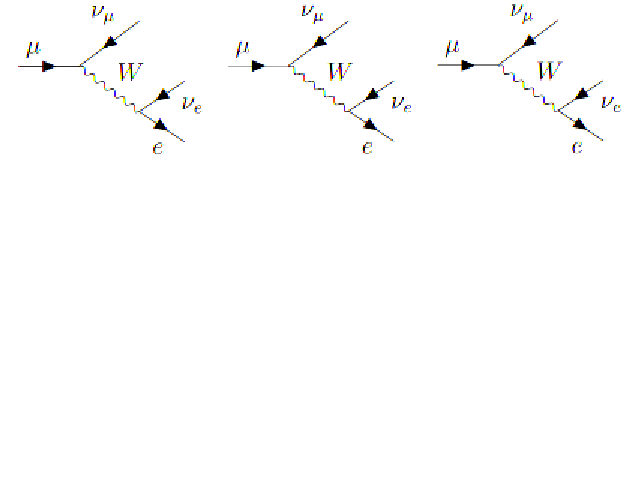
\includegraphics[width=0.5\textwidth]{Figures/5/mu_decay.pdf}
%		 \begin{tikzpicture}
%		 	\begin{feynman}
%		 		\vertex (a1); %mu
%
%		 		\vertex at ($(a1) + (1cm, 0)$) (b1); % decay to W+nu_mu
%				
%		 		\vertex at ($(b1) + (1, 0.75)$) (c1); %nu_mu
%				\vertex at ($(b1) + (1, -0.75)$) (c2); %W
%				
%				\vertex at ($(c2) + (0.75, 0.5)$) (d1); % nu_e
%				\vertex at ($(c2) + (0.75, -0.5)$) (d2); % e
%
%		 		\diagram* {
%		 		  (a1) -- [fermion, edge label=\(\mu\), near start] (b1),
%		 		  (c1) -- [fermion, edge label'=\(\nu_\mu\), near start] (b1) -- [boson, edge label=\(W\)] (c2),
%		 		  (d1) -- [fermion, edge label=\(\nu_e\), near start] (c2) -- [fermion, edge label'=\(e\), near end] (d2),
%		 		};
%		 	\end{feynman}
%		 \end{tikzpicture}
	\caption{Muon decay}
	\label{fig:muon_decay}
	\end{subfigure}
	\begin{subfigure}[t]{0.49\textwidth}
	\centering
	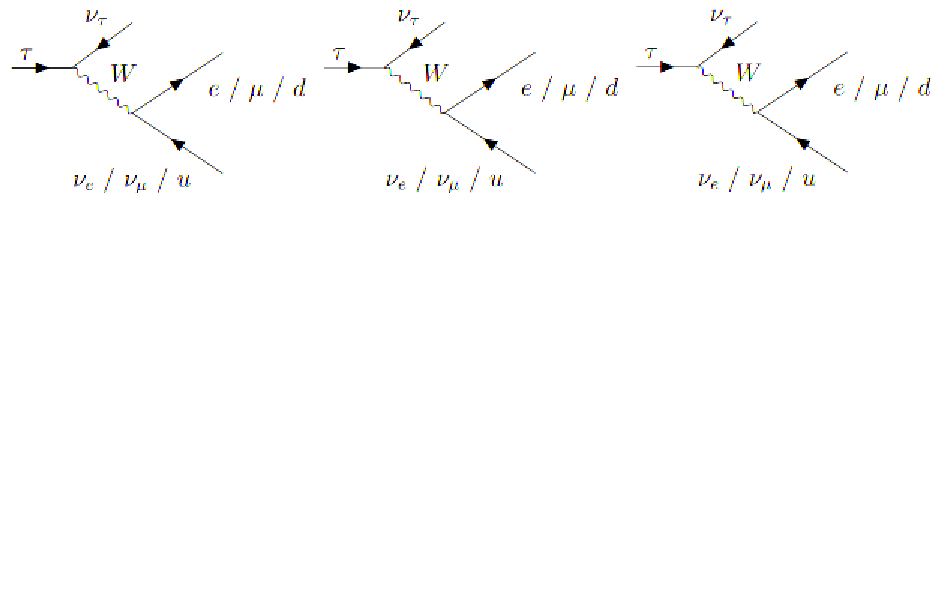
\includegraphics[width=0.75\textwidth]{Figures/5/tau_decays.pdf}
%		 \begin{tikzpicture}
%		 	\begin{feynman}
%		 		\vertex (a1); %tau
%
%		 		\vertex at ($(a1) + (1cm, 0)$) (b1); % decay to W+nu_tau
%				
%		 		\vertex at ($(b1) + (1, 0.75)$) (c1); %nu_tau
%				\vertex at ($(b1) + (1, -0.75)$) (c2); %W
%				
%				\vertex at ($(c2) + (1.5, -1)$) (d1); % nu_e / nu_mu / u / d
%				\vertex at ($(c2) + (1.5, 1)$) (d2); % e / mu / d / u
%
%		 		\diagram* {
%		 		  (a1) -- [fermion, edge label=\(\tau\), near start] (b1),
%		 		  (c1) -- [fermion, edge label'=\(\nu_\tau\), near start] (b1) -- [boson, edge label=\(W\)] (c2),
%		 		  (d1) -- [fermion, edge label={\(\nu_e\) / \(\nu_\mu\) / \(u\)}, near start] (c2) -- [fermion, edge label'={\(e\) / \(\mu\) / \(d\)}, near end] (d2),
%		 		};
%		 	\end{feynman}
%		 \end{tikzpicture}
	\caption{Tau decay}
	\label{fig:tau_decay}
	\end{subfigure}
	\caption{Decay mechanisms for muons and taus}
	\label{fig:lepton_decays}
\end{figure}

Due to their relatively large mass of 1.8 \GeV, taus can decay either leptonically to \(e\bar{\nu}_e\) or \(\mu\bar{\nu}_\mu\), or hadronically to \(d\bar{u}\), as shown in Figure \ref{fig:tau_decay}, and their decays proceed with a much shorter mean lifetime compared with the muon of 0.3ps. Because of this relatively short lifetime, taus will decay before passing through the ATLAS detector, and as such it is their leptonic or hadronic decay products that are actually measured in the detector. As will be discussed in Section \ref{sec:evt_selections} below, the selections applied for this analysis require that events have exactly one electron or muon in the final state in order to be considered for the search. As a result, the search is sensitive to \(s\rightarrow WW\) decays in which the leptonically decaying \(W\) decays to \(\tau\nu_\tau\) only in the case where the \(\tau\) decays leptonically to produce a single energetic electron or muon in the final state, which occurs with a 35\% branching fraction.

\subsubsection{Electrons}

As discussed in Section \ref{sec:EM_calo}, electron objects are reconstructed from clusters of energy deposits in the electromagnetic calorimeter that are associated with tracks in the inner detector, and calibrated to the EM scale. Detailed information about electron reconstruction, identification, and calibration can be found in Refs.~\cite{ATL-PHYS-PUB-2017-022}, \cite{PERF-2017-01} and \cite{PERF-2017-03}. To accommodate the differing needs of the various studies which make use of electron objects, ATLAS reconstructs these objects at several levels of identification and isolation efficiency, where these different efficiency levels are referred to as ``working points", and are typically referred to as variants of \emph{Loose}, \emph{Medium} and \emph{Tight} for reasons that will be discussed in the following paragraphs.

The identification efficiency refers to the probability that an electron passing through the detector will be correctly reconstructed and identified as such. In general, higher efficiency is achieved by loosening electron identification criteria, and comes at the cost of increased background acceptance. Increased background acceptance means that reconstructed objects have a higher probability of being incorrectly identified as having originated from an electron. 

Electron isolation tackles a slightly different, though related, challenge in comparison with identification. The goal of isolation is to separate the so-called ``prompt" electrons that are produced from the primary decay processes of heavy mediators produced in the \(pp\) collisions from background processes such as semileptonic quark decays, hadrons misidentified as leptons and photons that convert into \(e^+e^-\) pairs before reaching the EM calorimeter. It is generally found that reconstructed objects which originate from prompt electrons can be characterized by a relative absence of (i.e. isolation) from significant activity in a small angular radius in \(\eta\times\phi\) around the object. In analogue with the identification efficiency, a high isolation efficiency is achieved by loosening the criteria for defining an object as isolated. As such, prompt electrons have a high probability of being identified as isolated, but comes at the cost of an increased rate of incorrectly identifying objects which originate from background processes as isolated.
 
Two types of electrons are defined for the search based on different sets of criteria:
\newline \emph{Baseline} electrons use the \emph{Loose} working point for both identification and isolation. Isolation is measured within a fixed angular radius of \(\Delta R=0.2\) around the reconstructed electron object \cite{PERF-2017-01}. The \emph{Loose} identification working point is measured in dedicated studies performed within the ATLAS collaboration to have an efficiency of 93\% \cite{PERF-2017-01} for identifying prompt electrons with \(E_T=40~\GeV\). The \emph{Loose} isolation working point has a total measured efficiency of 98\% \cite{PERF-2017-01}. This electron definition has a relatively high efficiency, and is used to veto the presence of additional electrons in the final state.
\newline \emph{Signal} electrons are designed to be high-purity electrons. They are required to satisfy the \emph{Medium} identification criteria, which are measured to have an 88\% efficiency \cite{PERF-2017-01}, and \emph{Loose} isolation criteria.
\newline Both types of electrons require are required to have \(\pT > 7{\GeV} \) and a pseudorapidity in the range of \(|\eta| < 2.47\).

\subsubsection{Muons}

As described in Section \ref{sec:muon_spec}, muons are reconstructed using information from the the inner detector and the muon spectrometer. Detailed information about muon reconstruction, identification and calibration can be found in Refs. \cite{PERF-2015-10} and \cite{ATL-PHYS-PROC-2018-052}. In analogy to electron objects, muon objects are reconstructed at several identification and isolation working points, and two definitions for muons are considered for this analysis:
\newline \emph{Baseline} muons do not have any isolation requirement, and must satisfy the \emph{Loose} identification criteria, with a measured efficiency of 98\% for \(20~\GeV<p_{T, \mu}<100~\GeV\) \cite{PERF-2015-10}, for a high-efficiency selection.
\newline \emph{Signal} muons are designed to have a relatively high purity, and must satisfy the \emph{Medium} identification criteria, with a 98\% efficiency for \(20~\GeV<p_{T, \mu}<100~\GeV\) \cite{PERF-2015-10}. Signal muons are additionally required to pass a set of tight isolation criteria referred to as \emph{TightTrackOnly\_VarRad} \cite{ATL-PHYS-PROC-2018-052} which use information from the inner tracker, and are defined within an angular radius \(\Delta R\) around the reconstructed muon object that depends on the \pt of the muon object.
\newline Both types of muons use a threshold of \(\pt > 7~\GeV \). 

Baseline muons are required to have pseudorapidity in the range of  \(|\eta| < 2.7\). For signal muons, a tighter pseudorapidity range of \(|\eta| < 2.5\) is required to ensure that the muons are well measured in the inner detector as well as the muon spectrometer. 

\subsection{Small-radius \aktfour jets}
\label{sec:atk4_jets}

As discussed in detail in Section \ref{sec:had_calo}, quarks and gluons hadronize in the hadronic calorimeter to produce showers of energy deposits in the calorimeter known as jets. This search uses the ``particle flow algorithm" \cite{PERF-2015-09} to reconstruct objects associated with the resulting energy deposits. The particle flow algorithm matches signals from the inner tracker and the topologically connected clusters of energy deposits in the calorimeter referred to as ``topo-clusters" with the aim of forming objects representing individual charged particles. The energy deposited in the calorimeter by these identified charged particle objects is, leaving behind an ensemble of ``particle flow objects" consisting of the remaining calorimeter energy and tracks which are matched to the hard interaction. The anti-\(k_t\) algorithm described in Ref. \cite{akt_algo} is then used to reconstruct jets using these particle flow objects. Various angular jet radii \(R\), where \(R\) is defined in Eq. \ref{eq:jet_radius}, may be considered for jet reconstruction depending on the kinematics and anticipated origins of the quark or gluon which initiated the shower (see discussion in Section \ref{sec:had_calo} for more details), where \(R\) determines the angular radius within which the anti-\(k_t\) algorithm includes calorimeter deposits for jet reconstruction. 

As discussed in Chapter \ref{chapter:dh_model}, the final state signature of DH model targeted in this search involves a pair of energetic \(W\) bosons in the final state, one of which decays leptonically to a \(\ell\nu\) pair, and the other hadronically to a pair of quarks. If the boost of the hadronically decaying \(W\) is sufficiently low, the two quarks may have a large enough angular separation as to be most effectively reconstructed as two separate jets with small radius. In the so-called ``resolved" regime of the search, the quark-induced jets so resolved that it is not even possible to reconstruct them as a single multi-pronged large-radius jet. For this search, these so-called ``\smallR" jets are reconstructed with a radius of \(R=0.4\).

After the \smallR jets are reconstructed are fully calibrated \cite{ATLAS-CONF-2015-037}, only jets with \(\pt > 20~\GeV\) and \(|\eta| < 2.5\) are considered for the search. Jet cleaning \cite{ATLAS-CONF-2015-029} with the \emph{TightBad} working point is applied to suppress noise in the calorimeter and background jets which are not produced from the primary \(pp\) collision. The jet vertex tagger \cite{ATLAS-CONF-2014-018} is applied with the \emph{Tight} working point to suppress pileup jets \cite{pileup} from other \(pp\) interactions in the same and neighbouring bunch crossings - see Section \ref{sec:evt_wts} for a more detailed discussion of pileup events. As described in Section \ref{sec:resolved_w_cand} below, these jets are used in the analysis to identify quarks originating from the hadronically-decaying \(W\) boson in the DH signal model in the resolved regime, and to reconstruct the \(W\) boson in this regime.

\subsubsection*{\btag}
\label{sec:btag}
\btagged jets are identified with the \verb|DL1r| algorithm \cite{ATLAS-CONF-2018-006}, which uses a deep learning method for the identification. A fixed working point with 77\% efficiency is used. \btagged jets are vetoed in the signal region to reduce the background of SM \ttbar and single-top processes (see Section \ref{sec:dominant_bkgs} for details).

\subsection{Resolved \(W\) Candidate}
\label{sec:resolved_w_cand}

As described in Section \ref{sec:atk4_jets} above, the pair of quarks produced by the hadronic decay of the \(W\) boson in the signal model are reconstructed as two resolved \smallR jets in the less-boosted resolved regime. The parent \(W\) boson can then be reconstructed from \smallR jets induced by its daughter quarks using the combined energy and momentum of the \smallR jet pair. Given that \smallR jets can also be produced by, for example, initial-state radiation and pileup, it is quite common for there to be more than two \smallR jets reconstructed in the final state. These additional \smallR jets introduce some ambiguity in terms of identifying which \smallR jets reconstructed in the final state should be associated with the hadronic decay of a \(W\) in the signal model. For events with more than two \smallR jets in the final state, the pair of \smallR jets whose combined invariant mass is closest to the \(W\) boson mass are associated with the \(W\) decay products, and used to reconstruct the \(W\) boson candidate. The algorithm for this jet identification and \(W\) boson reconstruction so is as follows:

\begin{itemize}
\item Construct all possible combinations of two \smallR jets (a.k.a. ``dijet pairs") in the final state.
\item For each such candidate dijet pair, \(j_1\) and \(j_2\), sum the four-momenta of the reconstructed jets, \(\mathbf{p}_{j_1,j_2} = \mathbf{p}_{j_1} + \mathbf{p}_{j_2}\), and calculate their combined invariant mass: 

\begin{equation}
\label{eq:dijet_invt_mass}
M_{j_1,j_2} = \sqrt{\mathbf{p}_{j_1,j_2} \cdot \mathbf{p}_{j_1,j_2} } 
\end{equation}
\item Select the dijet pair whose invariant mass is closest to the \(W\) boson mass of \(80.4~\GeV\) \cite{PDG_2018} as the \smallR jets to be associated with the \(W\rightarrow q\bar{q}\) decay.
\item Reconstruct the candidate hadronically decaying \(W\) boson using the dijet pair with four-momentum \(\mathbf{p}_{j_1,j_2}\).
\end{itemize}

Figure \ref{fig:resolved_Wmass_reco} shows distributions of the reconstructed mass of the \(W\) boson candidate for MC simulated events generated at a range of sample \ms and \mZp after application of the baseline event selections presented in Section \ref{sec:evt_selections}, with the additional requirement that there be at least two \smallR jets in the final state. The distributions are in general well centred around the \(W\) boson mass.

\begin{figure}[h]
	\centering
	\begin{subfigure}[b]{0.49\textwidth}
	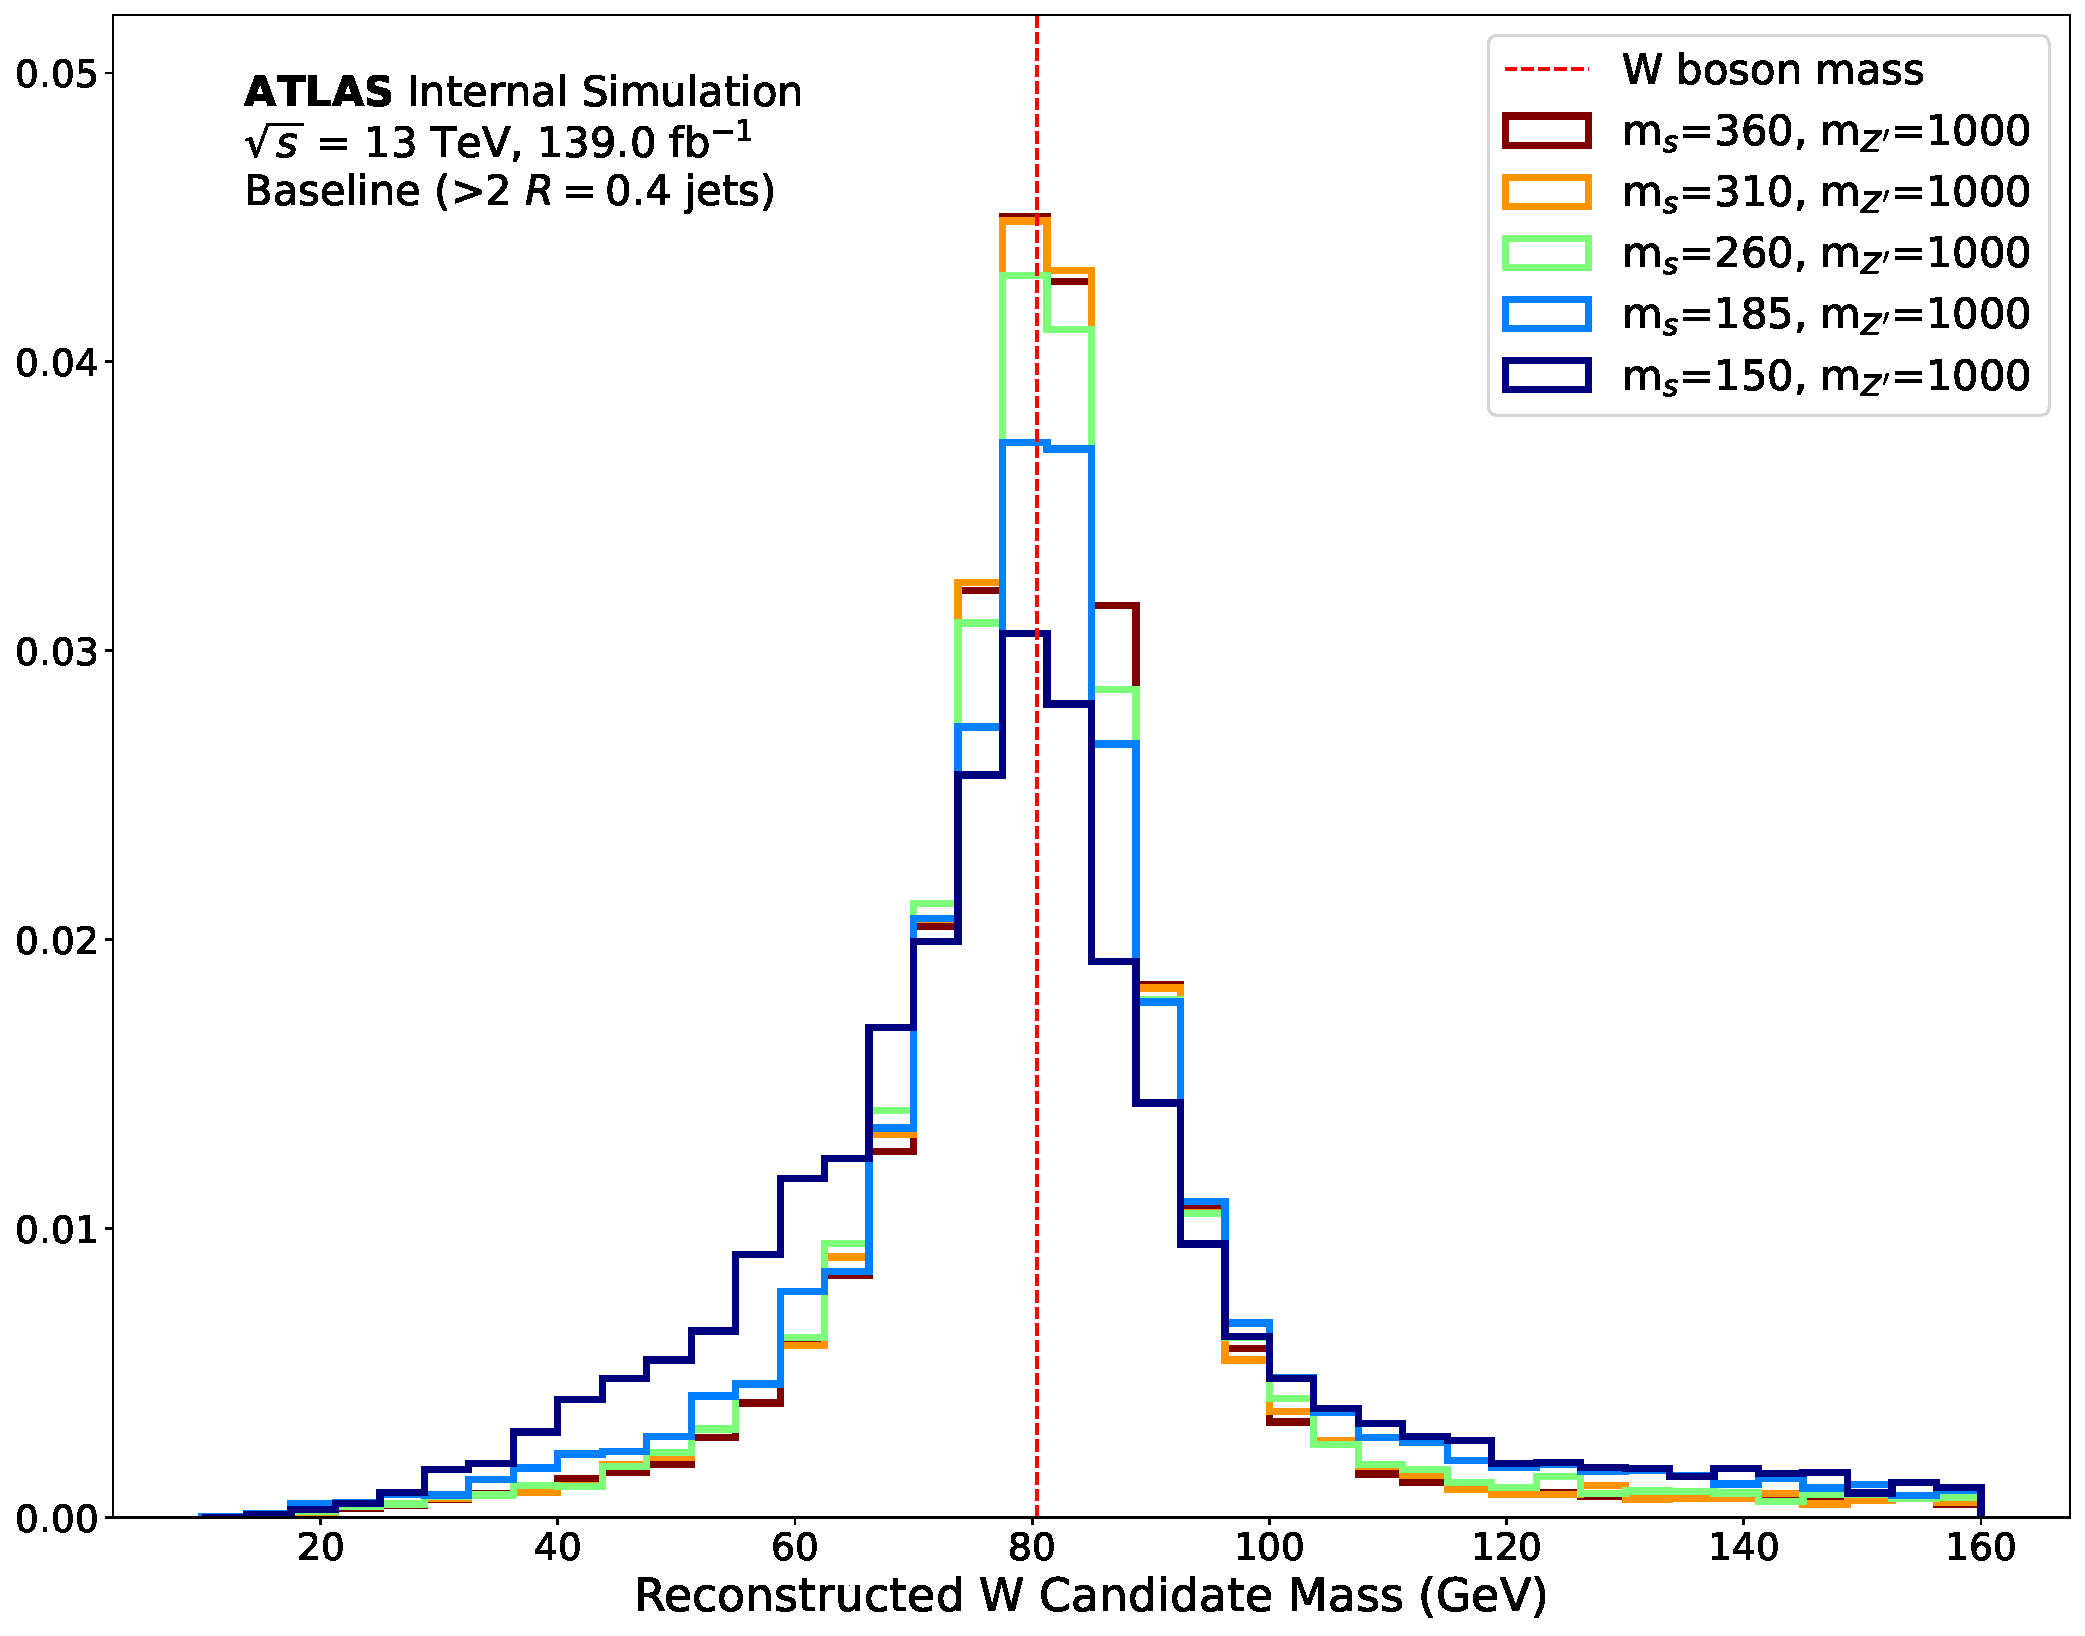
\includegraphics[width=0.95\textwidth]{Figures/5/WCand_m_ms.pdf}
	\caption{\mZp Fixed, \ms Varied}
	\label{fig:resolved_Wmass_reco_ms}
	\end{subfigure}
	\begin{subfigure}[b]{0.49\textwidth}
	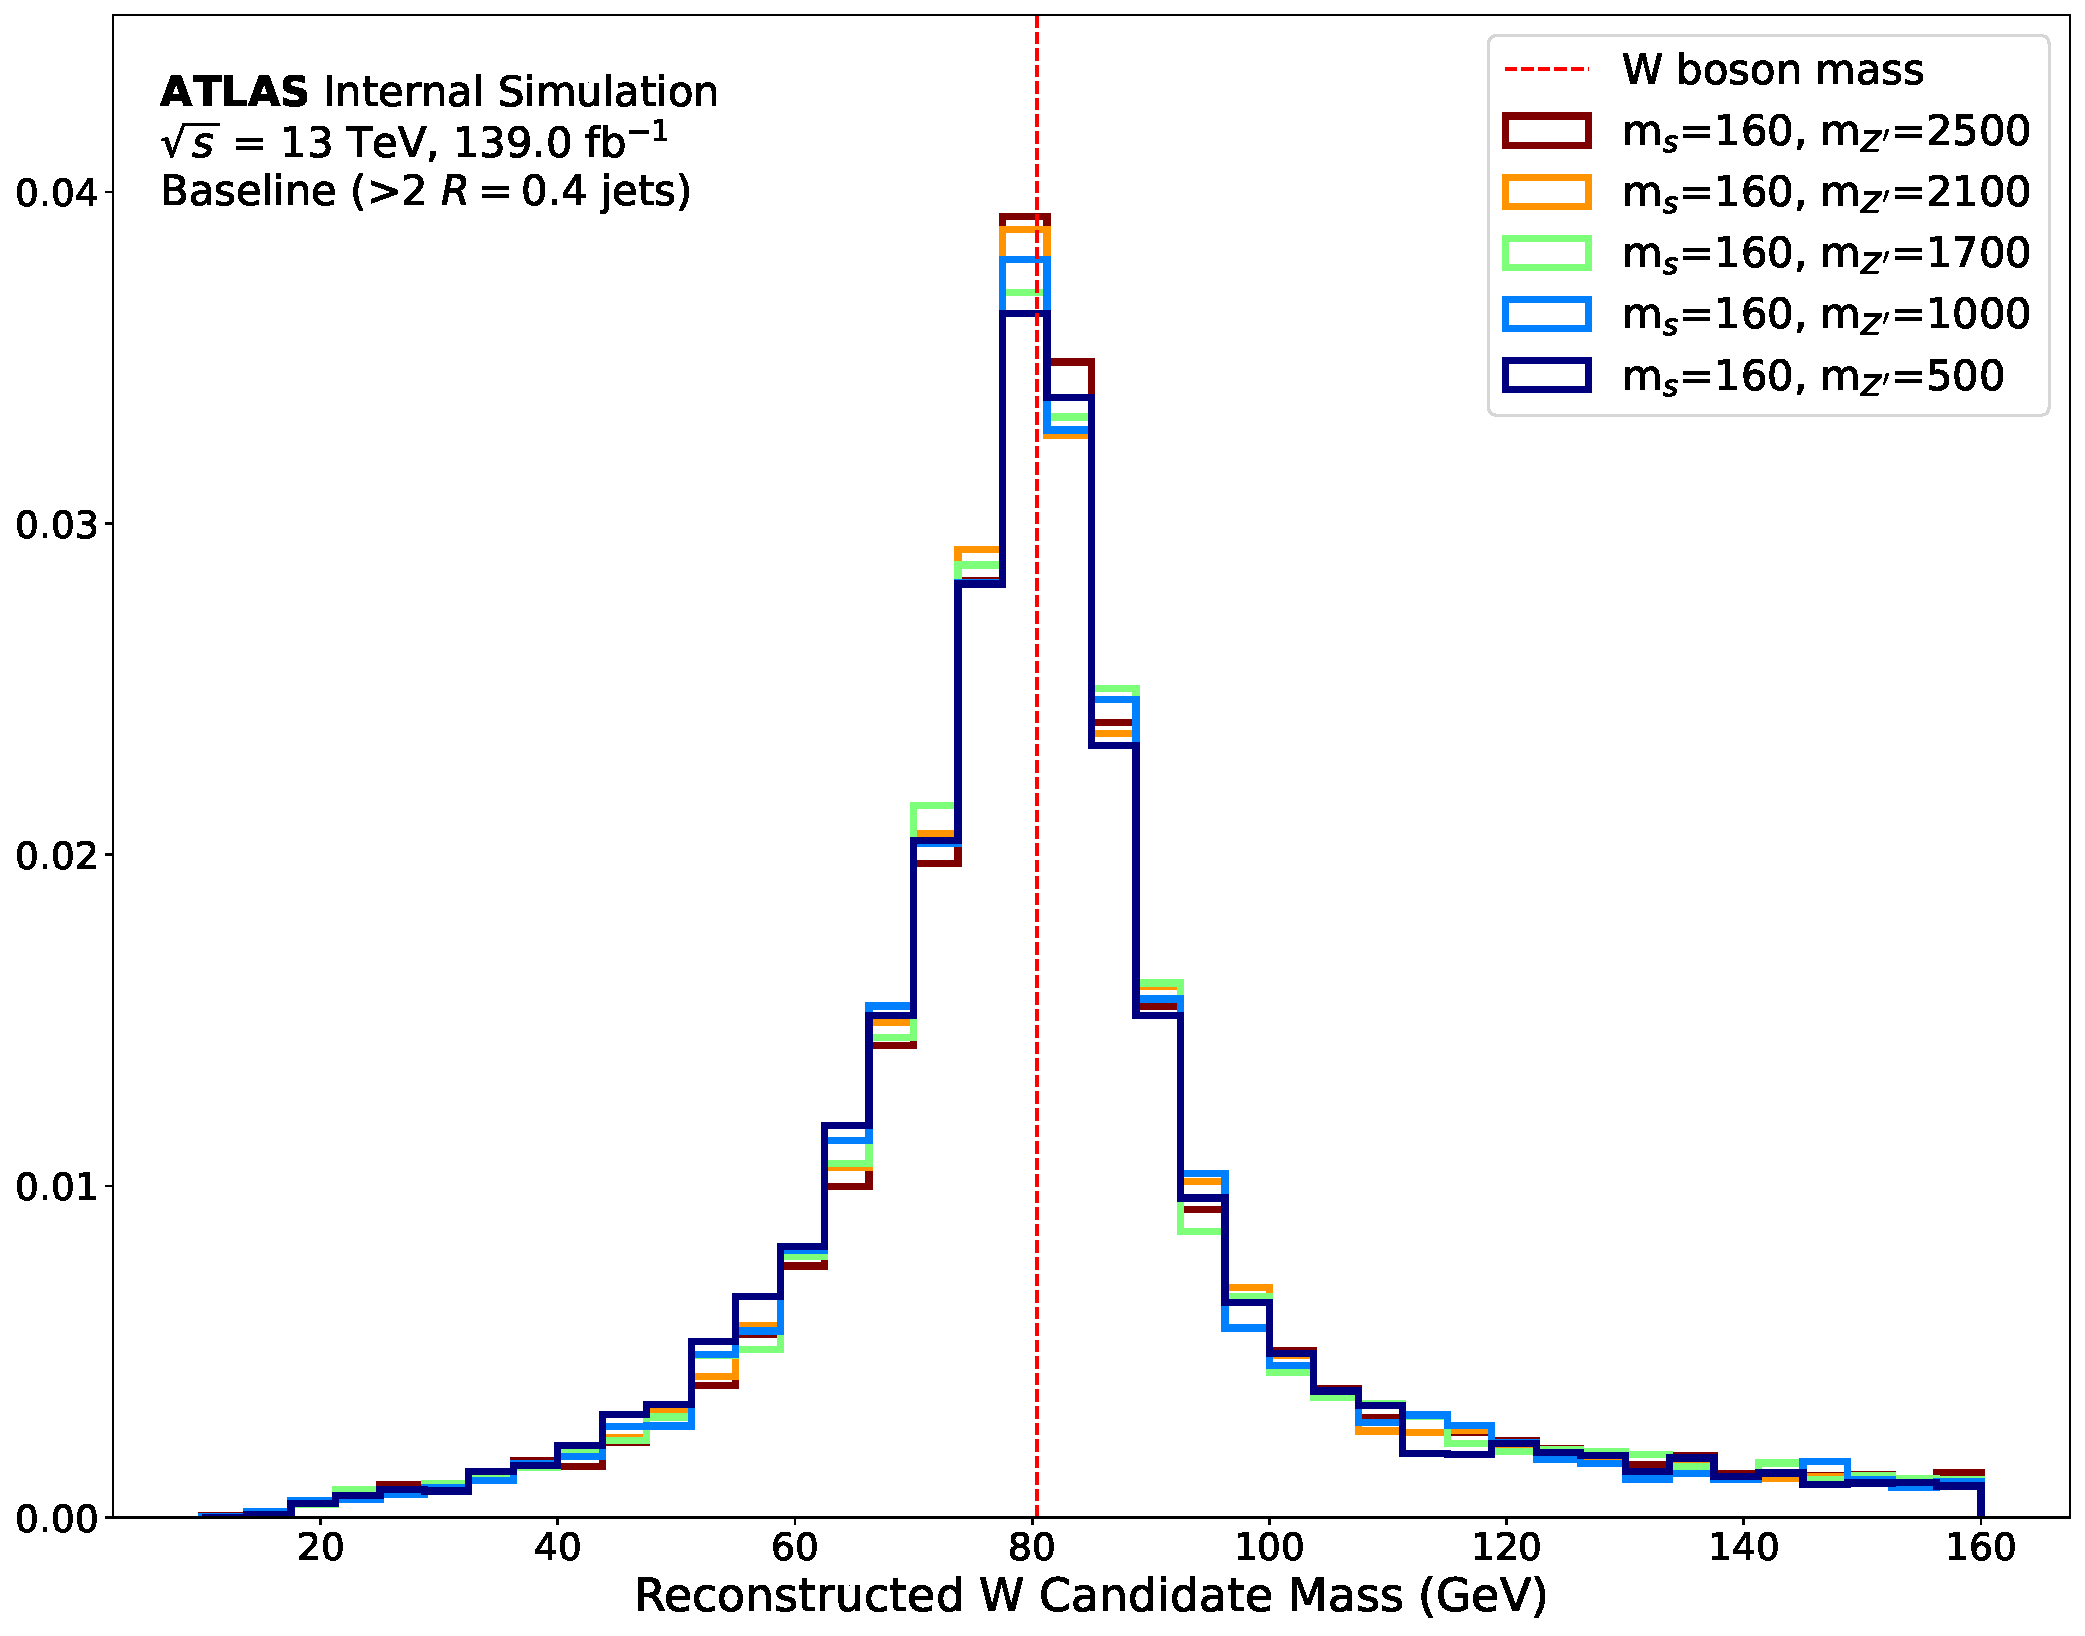
\includegraphics[width=0.95\textwidth]{Figures/5/WCand_m_mZp.pdf}
	\caption{\ms Fixed, \mZp Varied}
	\label{fig:resolved_Wmass_reco_mZp}
	\end{subfigure}
	\caption[]{Distributions of the reconstructed W candidate mass for MC simulated events produced for the DH signal model over a range of \ms and \mZp. All events included in the distributions are required to pass the baseline event selection described in Section \ref{sec:evt_selections} is applied, and to have at least two \smallR jets in the final state. The red dashed vertical line is placed at the \(W\) boson mass of 80.4 \GeV. Distributions are normalized to unit area.}
	\label{fig:resolved_Wmass_reco}
\end{figure}

\subsection{Track-Assisted Reclustered Jets (Merged \(W\) Candidate)}
\label{sec:TAR_jets}

If the hadronically decaying \(W\) boson is produced with a sufficiently large momentum (i.e. boost), the jets produced by the \(q\) pair may be sufficiently collimated (i.e. ``merged") that they are most effectively reconstructed as a single multi-pronged large-radius jet, as opposed to the resolved \smallR jets used for \(W\) reconstruction in the resolved regime (see Sections \ref{sec:atk4_jets} and \ref{sec:resolved_w_cand} above for details). 

Since the signal model predicts that charged particle tracks and energy deposits in the detector will have originated primarily from the two quarks produced by the \(W\rightarrow q\bar{q}\) decay in the signal model, it is important to reconstruct the large-radius jet in this so-called merged regime with as much detailed kinematics and substructure information as possible, in order to identify features that would be consistent with the jet containing tracks and energy deposits originating from two energetic quarks originating from a \(W\) parent. Such features would include the combined invariant mass \mTAR of all particles which produced the jet, which would be expected to be consistent with the \(W\) boson mass within detector resolution. Important substructure information would include variables which aim to quantify the number of distinct ``prongs" of localized energy deposition within the jet, which can be correlated to the number of high-\pt strongly interacting particles whose energy deposits are included in the jet (two such prongs would be expected for the signal model). 

This search uses the track-assisted reclustered (TAR) jet algorithm \cite{ATL-PHYS-PUB-2018-012} for large-radius jet reconstruction in the merged regime. In this regime, the highest-\pt TAR jet reconstructed with a radius parameter of \(R=1.0\) is identified as the physics object which constitutes the the decay products of the candidate hadronically decaying \(W\) boson (\(W_\text{had}\)) in the DH signal model. Whereas most large-radius jet reconstruction techniques rely on energy deposits in the calorimeter to construct the jet substructure information, TAR jets are designed to combine charged particle tracks measured by the inner tracker with the calorimeter energy deposits to obtain a higher-resolution construction of TAR substructure information, taking advantage of the superior resolution of the inner tracker compared with calorimeter. 

\subsubsection{TAR Algorithm}
\label{sec:TAR_algo}

For this search, \(R=0.2\) \smallR jets are used to reconstruct energy deposits in the calorimeter, and are input to the TAR algorithm along with tracks measured by the inner detector which satisfy a set of quality criteria summarized in Table \ref{tab:TARparameters}. The TAR algorithm \cite{ATL-PHYS-PUB-2018-012} is as follows: the input \(R=0.2\) \smallR ``subjets" are reclustered using the \akt algorithm with \(R=1.0\) to \largeR jets. A trimming procedure is applied to mitigate the effects of pileup and background QCD processes within the triggered event that do not originate from the hard interaction. The trimming procedure removes any of the input subjets which carry less than a fraction \(\fcut=0.05\) of the total transverse momentum of the \largeR jet: \(\pt^\text{subjet}/\pt^\text{\largeR jet} < 0.05\).  The tracks from the inner detector are then matched to the remaining \smallR subjets using the ghost association procedure described in Ref. \cite{ghost_association_2008}, if possible. Any tracks which cannot be matched to subjets using ghost association are instead matched to the nearest subjet, provided that there is a jet within an angular radius \(\Delta R=0.3\) of the track. To account for the energy of the neutral hadronic jet components which do not leave tracks in the inner detector, the \pt of each track is scaled such that the \(\pt\)s of all tracks matched to a given subjet will sum to the energy of the subjet measured by the calorimeter:

\begin{equation}
\label{eq:tar_track_pt_scaling}
\pt^\text{track, new} = \pt^\text{track, old} \times \frac{p_{T,j}^\text{subjet}}{\sum_{i \in j}p_{T, i}^\text{track, old}}
\end{equation}

\noindent where the index \(i\) runs over all tracks matched to the subjet \(j\). The rescaled tracks and remaining subjets are again reclustered using the \akt algorithm to form the final \largeR TAR jet.

While the kinematic properties of the TAR jets are calculated from the constituent \smallR jets, the jet substructure as well as the mass \(m^\text{TAR}\) are calculated from the constituent tracks. Figure \ref{fig:TARAlg} shows a visual summary of the basic TAR algorithm. 

\subsubsection{TAR-lepton Disentanglement}

The analysis uses the TAR algorithm on \(R=0.2\) \smallR jets and tracks that have undergone a ``TAR-lepton disentanglement" preselection to remove tracks associated with any reconstructed baseline electrons or muons and any \(R=0.2\) jets which overlapped with the baseline electron tracks. This preselection is helpful in this analysis because the charged lepton produced by the leptonic \(W\rightarrow \ell\nu\) decay often falls within the \(R=1.0\) cone of the TAR jet, as illustrated in Figure \ref{fig:TAR_lepton_overlap_illustration}, and disrupts the jet reconstruction, particularly by means of additional jet energy induced by calorimetric clusters created by an overlapping electron.

\begin{figure}[H]
  \centering
     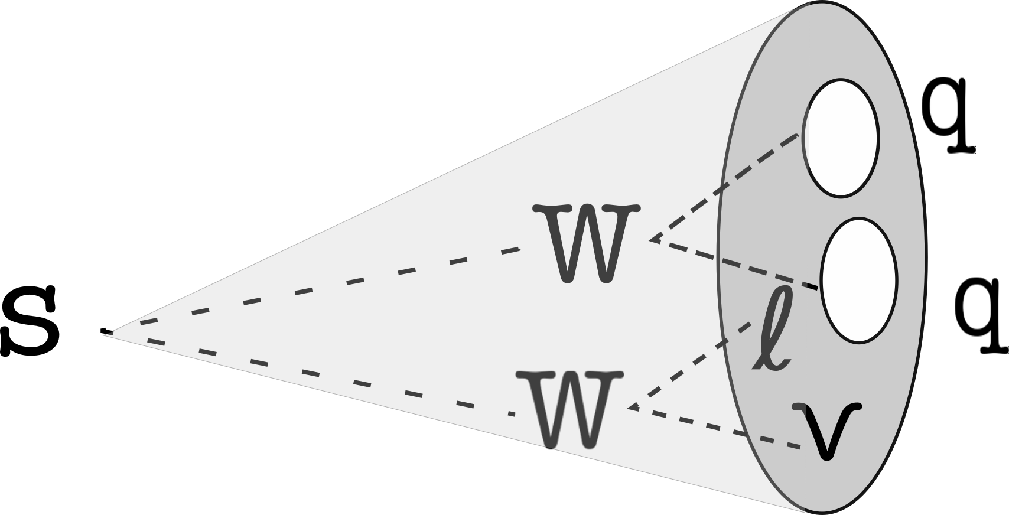
\includegraphics[width = 0.3\textwidth]{Figures/5/lepton_overlap.pdf}
     \caption{Illustration of the final state scenario in which the charged lepton produced by the leptonic \(W\rightarrow \ell\nu\) decay overlaps with the \largeR TAR jet reconstructed from the hadronic \(W\rightarrow qq\) decay.}
     \label{fig:TAR_lepton_overlap_illustration}
  \end{figure}
  
Figure \ref{fig:TARdisentaglementplots} shows a comparison of the distributions of reconstructed TAR jet mass \mTAR either without or with the TAR-lepton disentanglement preselection applied, for MC simulated events produced for the DH signal model at several representative \ms and \mZp, in which the reconstructed electron in the final state overlaps with the highest-\pt reconstructed TAR jet. For all the signal points, the TAR-lepton disentanglement preselection is found to substantially improve the ability of the TAR algorithm to reconstruct TAR jets with \mTAR near the \(W\) boson mass, as would be expected for the signal model.
  
\begin{figure}[H]
\centering
\begin{subfigure}{0.49\textwidth}
   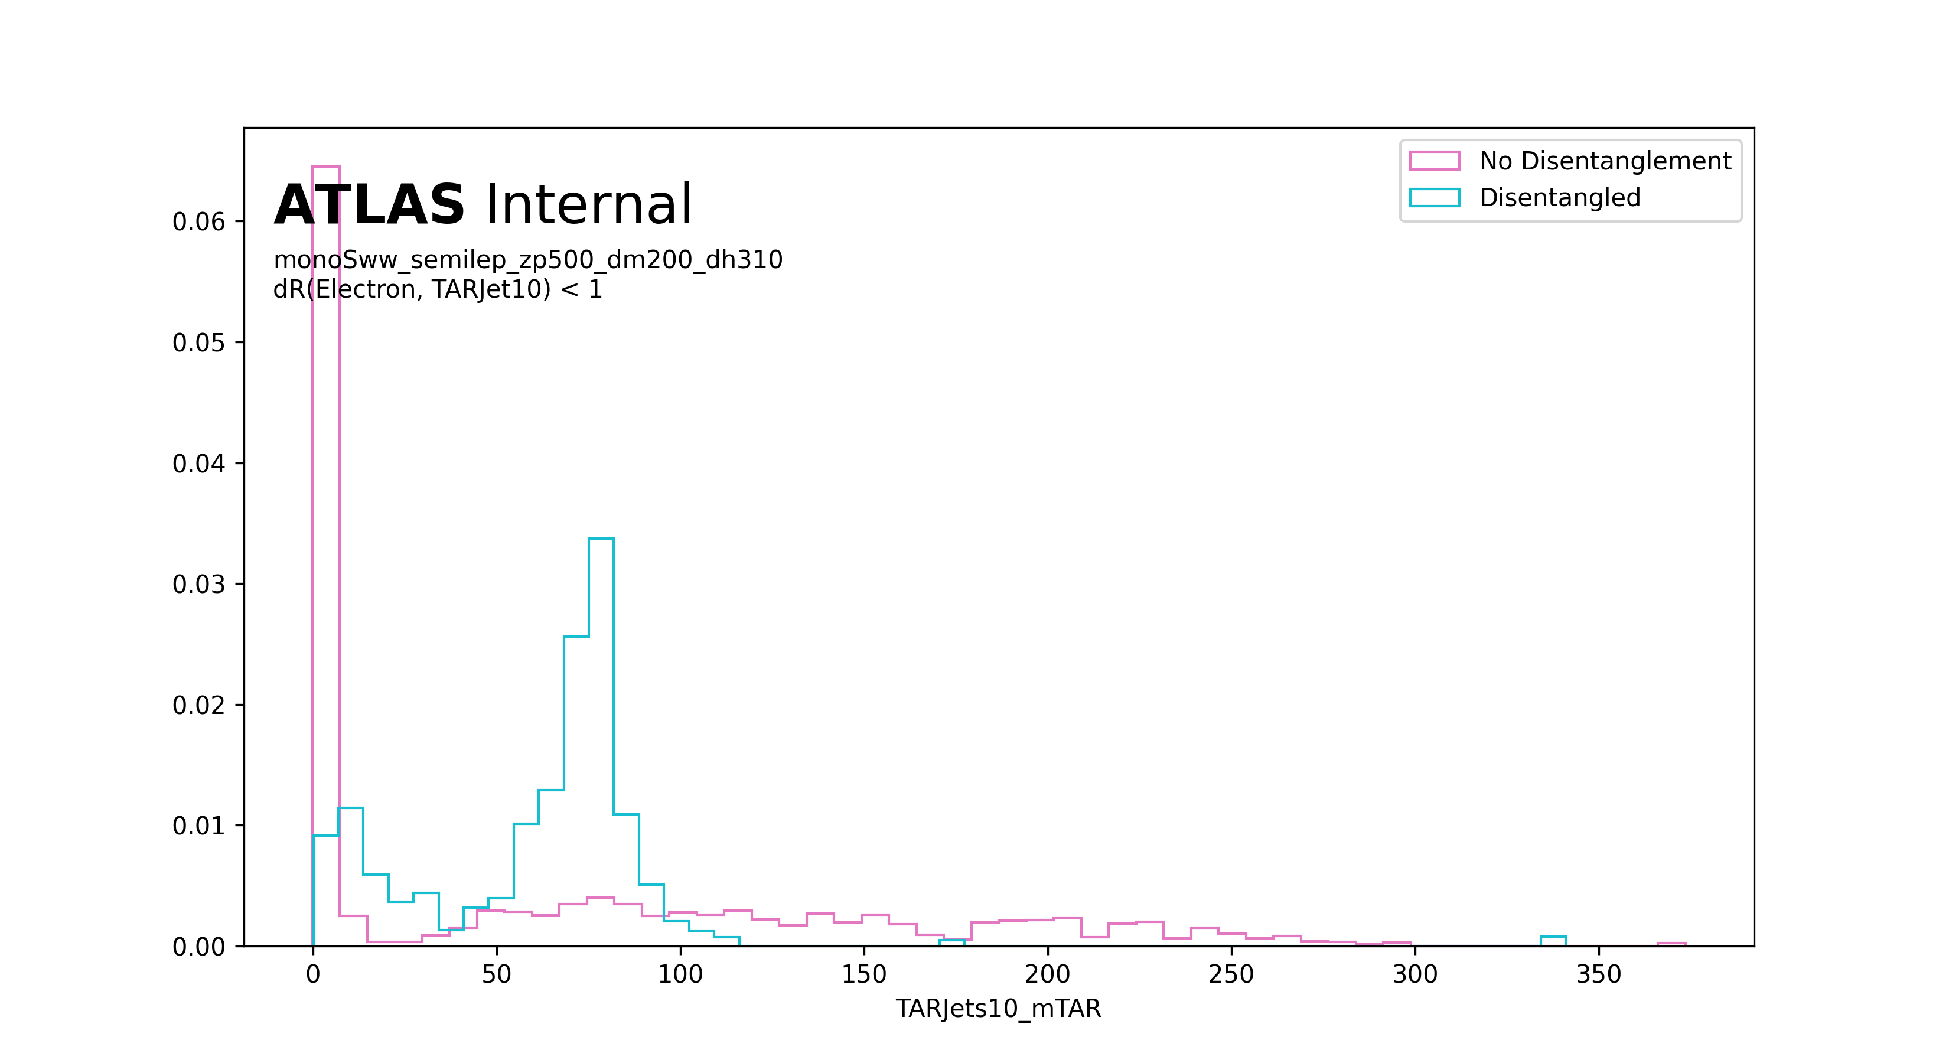
\includegraphics[width = 0.95\textwidth]{Figures/5/monoSww_semilep_zp500_dm200_dh310.pdf}
   \caption{\((\ms, mZp) = (310, 500)~\GeV\)}
   \label{fig:TARdisentaglementplots_zp500_dh310}
\end{subfigure}
\begin{subfigure}{0.49\textwidth}
   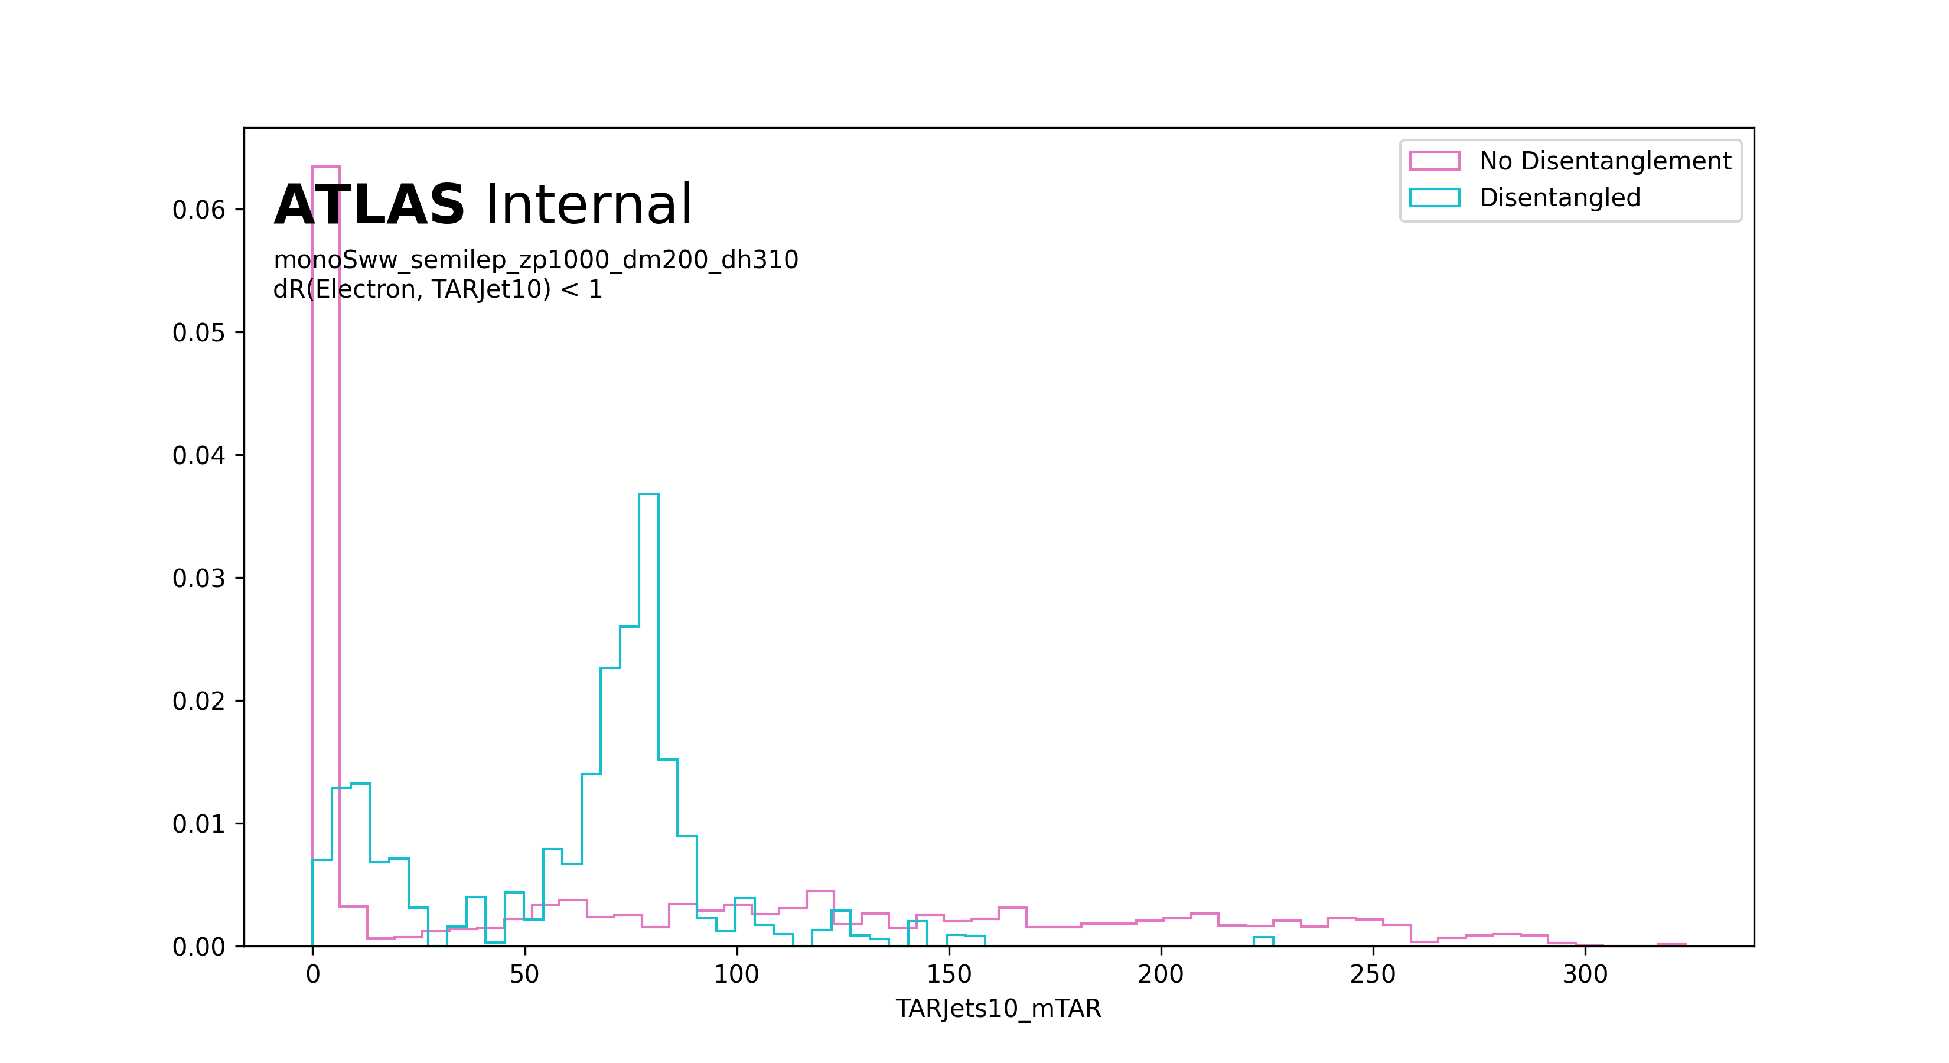
\includegraphics[width = 0.95\textwidth]{Figures/5/monoSww_semilep_zp1000_dm200_dh310.pdf}
   \caption{\((\ms, mZp) = (310, 1000)~\GeV\)}
   \label{fig:TARdisentaglementplots_zp1000_dh310}
\end{subfigure}
\begin{subfigure}{0.49\textwidth}
   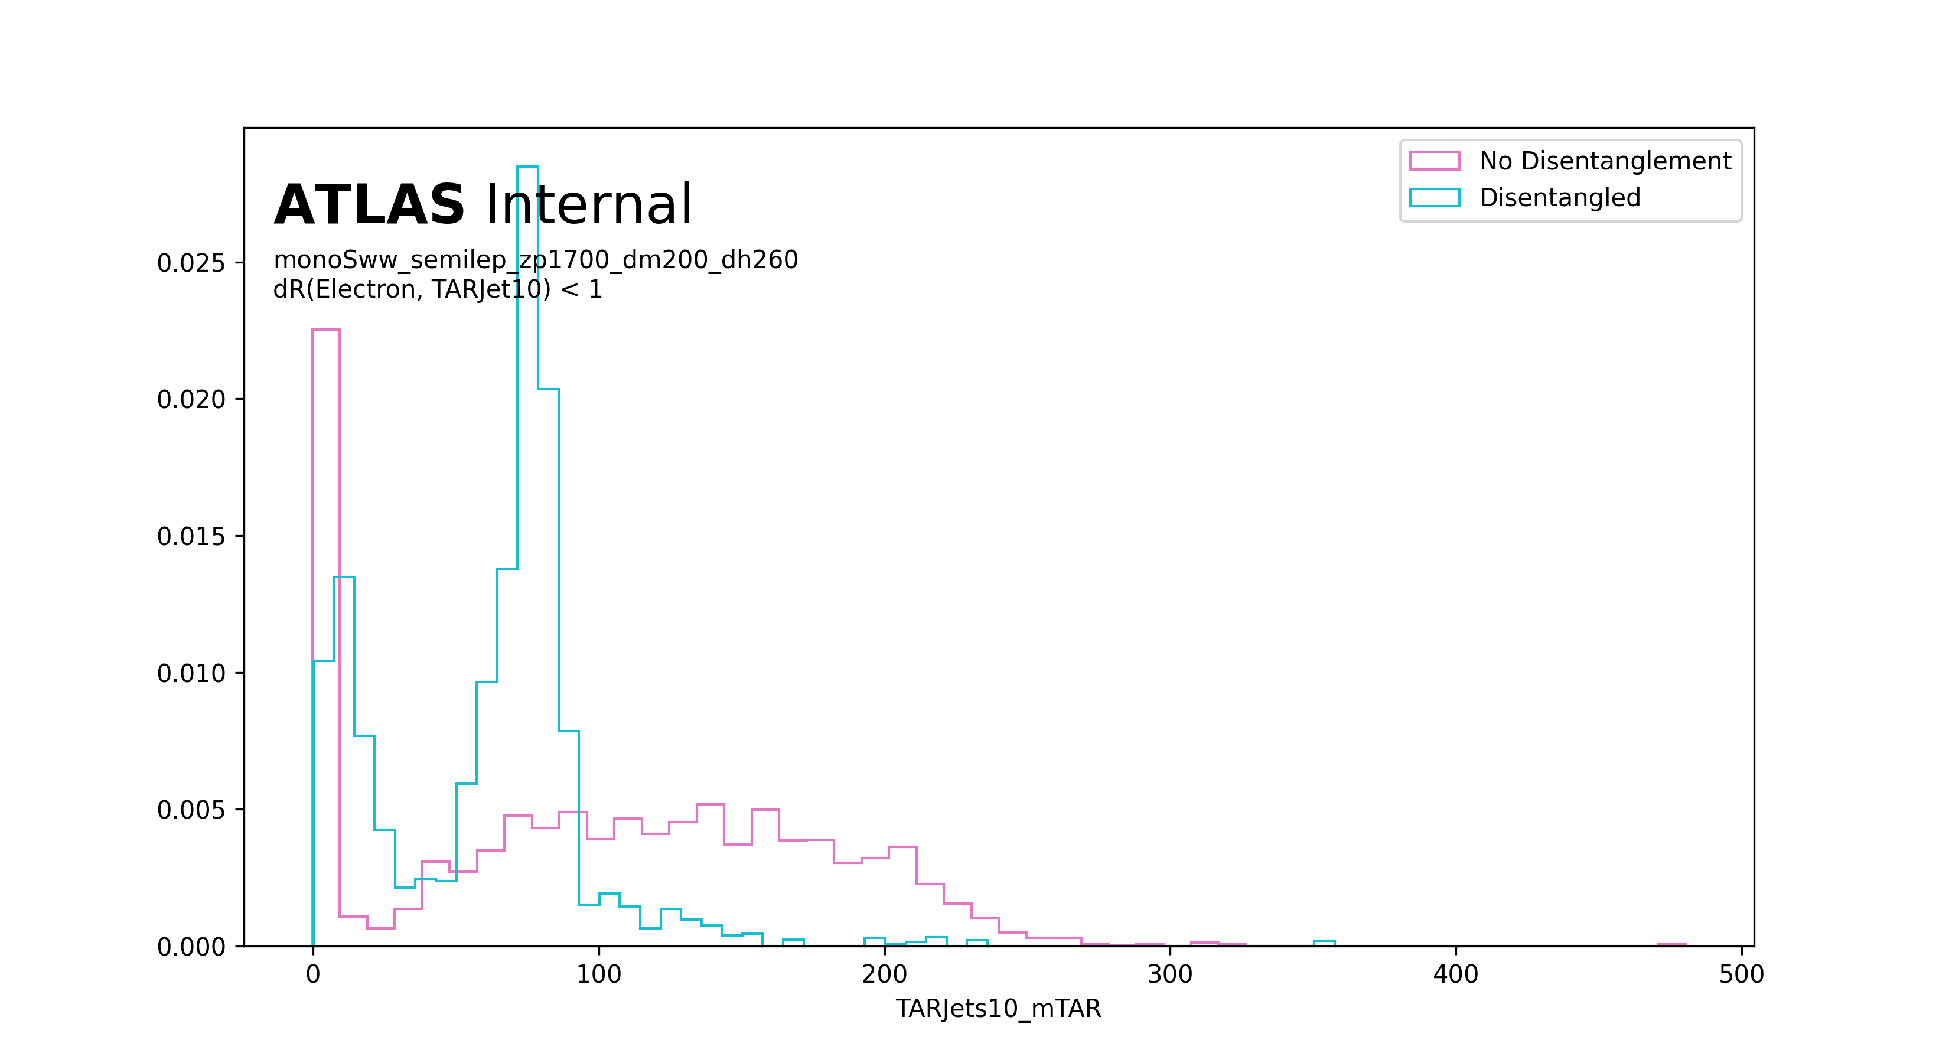
\includegraphics[width = 0.95\textwidth]{Figures/5/monoSww_semilep_zp1700_dm200_dh260.pdf}
   \caption{\((\ms, mZp) = (260, 1700)~\GeV\)}
   \label{fig:TARdisentaglementplots_zp1700_dh260}
\end{subfigure}
\begin{subfigure}{0.49\textwidth}
   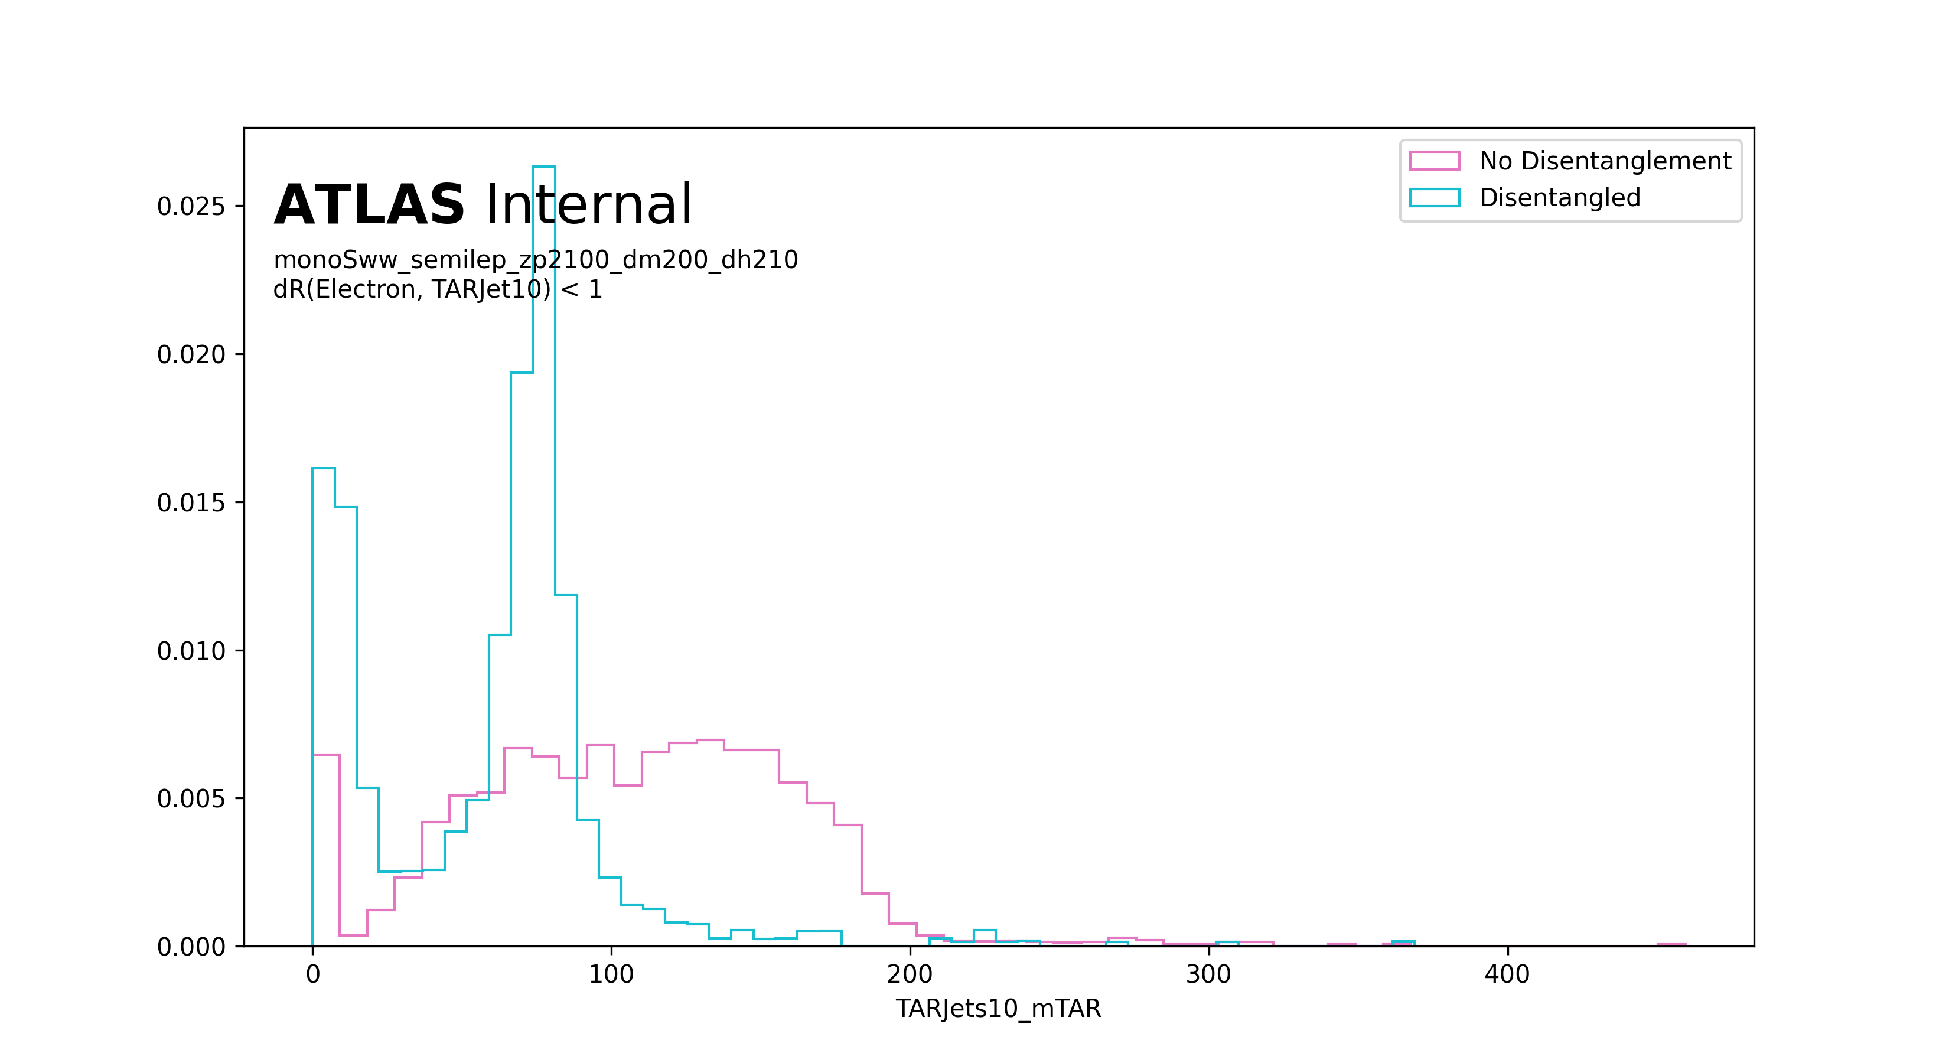
\includegraphics[width = 0.95\textwidth]{Figures/5/monoSww_semilep_zp2100_dm200_dh210.pdf}
   \caption{\((\ms, mZp) = (210, 2100)~\GeV\)}
   \label{fig:TARdisentaglementplots_zp2100_dh210}
\end{subfigure}
   \caption{Distributions of \mTAR for the leading-\pt TAR jet in MC simulated events generated for the DH signal model process with semileptonic \(WW\) decay at several representative \ms and \mZp, with and without application of the lepton disentanglement preselection. Events included in the distributions are required to pass the baseline selection requirements presented in Section \ref{evt_selections}, and to have one signal electron and at least one reconstructed TAR jet. Distributions are normalized to unit area.}
   \label{fig:TARdisentaglementplots}
\end{figure}

\subsubsection{Summary of the TAR Procedure}

The following steps summarize the algorithm used to construct the TAR jets used in this search (steps with a * are added to disentangle leptons):
\begin{itemize}
  \item Tracks and calibrated \akt \(R=0.2\) jets are chosen as input to the algorithm.
  \item Tracks associated with a baseline muon or electron are removed from the input collection (*).
  \item \(R=0.2\) jets overlapping with a baseline electron (\(\DeltaR<0.2\)) are removed from the input collection to the TAR algorithm (*).
  \item The remaining \(R=0.2\) subjets are reclustered using the \akt algorithm into \(R=1.0\) jets and trimmed using the \(p_T\) fraction \(\fcut=0.05\).
  \item Input tracks are matched to \(R=0.2\) subjets which remain after trimming, if possible, using ghost association.
  \item Tracks which remain unassociated are matched to the nearest \akt \(R=0.2\) jet within \(\DeltaR<0.3\).
  \item The \pt of each track is rescaled using the \pt of the jet to which it is matched using Eq. \ref{eq:tar_track_pt_scaling}. This rescaling accounts for the missing neutral momentum, which is measured at calorimeter level but is not present at tracker level.
  \item Finally, jet substructure variables and  \(m^\text{TAR}\) are calculated using the rescaled matched tracks.
\end{itemize}
The parameters of the TAR algorithm used are summarized in Table \ref{tab:TARparameters}. \\

\begin{figure}[htb]
  \centering
     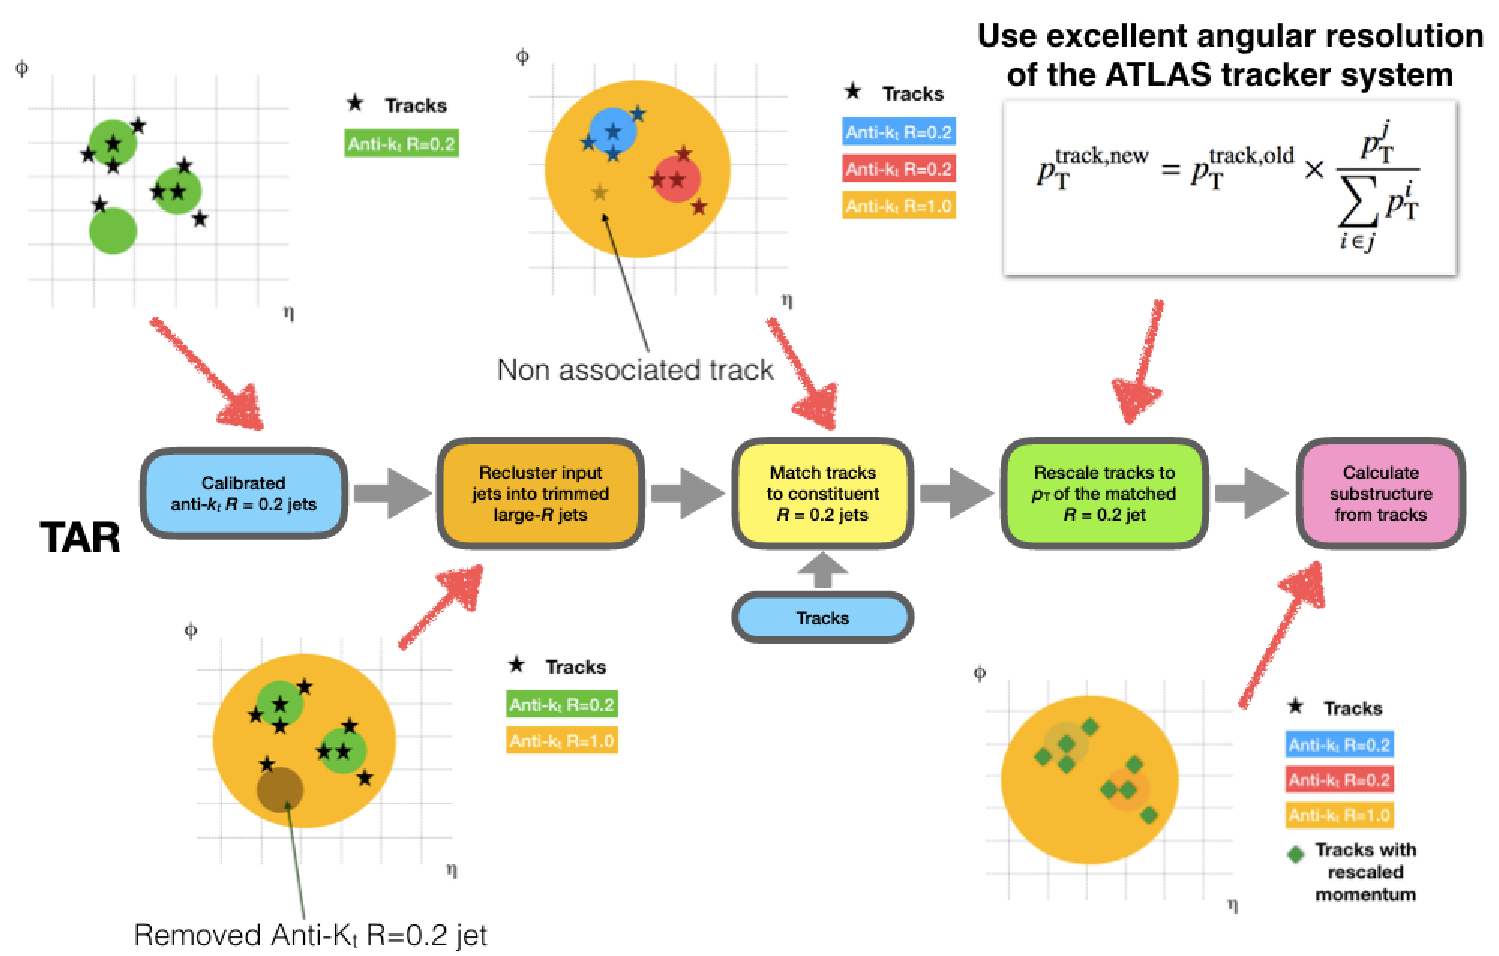
\includegraphics[width = 0.80\textwidth]{Figures/5/TARJetdescription.pdf}
     \caption{TAR jet reconstruction algorithm depicted without lepton disentanglement. Figure adapted from \(\copyright\) \cite{ATL-PHYS-PUB-2018-012}}
     \label{fig:TARAlg}
  \end{figure}

\begin{table}[htbp]
\centering
\caption{TAR jet reconstruction parameters}
\label{tab:TARparameters}
\begin{tabular}{l l }
\toprule
\multirow{3}{*}{Track selection} & \verb|Loose| quality\\
	& \(\pt > 0.5~\GeV\) \\
	& \(|\eta| < 2.5\)  \\
Tracks removed if associated to & electrons, muons \\
\midrule
\multirow{3}{*}{Input jet selection} & \(R=0.2\) \akt jets \\
	& \(\pt > 20~\GeV\) \\
	&  \(|\eta| < 2.5\)  \\
\midrule
Reclustering radius & \(R=1.0\) \\
TAR jet \pt & \(\pt^\text{TAR} > 100~\GeV\) \\
Trimming radius & \(R=0.2\) \\
Trimming \pt fraction & \(f_\text{cut}=0.05\) \\
Track-to-jet association & \(\DeltaR(\text{jet, track}) < 0.3\) \\
jet-electron overlap removal & \(\DeltaR(\text{jet, electron}) < 0.2\) \\
\bottomrule
\end{tabular}
\end{table}

\subsection{\met}
\label{sec:met_object_description}

The missing transverse momentum \met, introduced in Section \ref{sec:met}, quantifies the imbalance of momentum in the plane transverse to the beam line. If all particles produced in a \(pp\) collision are fully detected, conservation of momentum implies that the transverse momenta of all objects produced by the event should sum to zero within detector resolution. As a result, large \met in an event is indicative of the production of undetected energetic particles. The semileptonic \(s\rightarrow WW(qq\ell\nu)\) decay channel of the LHC signature for the DH model probed in this DM search (see Chapter \ref{chapter:dh_model} for details) predicts large (i.e. above-detector-resolution) \met in the final state. The large \met would be due to both the DM pair produced from from the decay of the hypothetical \Zprime, as well as the neutrino produced by the leptonic decay of one of the \(W\) bosons in the final state. Both the DM pair and the neutrino would be expected to pass through the detector without any appreciable interactions due to their very low interaction cross sections with SM particles, and hence constitute undetected (i.e. missing) momentum in the event.

The \met is calculated using fully calibrated and reconstructed physics objects \cite{PERF-2016-07}. For this analysis, \met terms from baseline electrons and muons (see \Sect{\ref{sec:charged_leptons}}) and \(R=0.4\) jets (see \Sect{\ref{sec:atk4_jets}}) are used. In addition, a soft term calculated from tracks that are not associated with any of these reconstructed objects is added. Reconstructed \(\tau\)-leptons and photons are not considered in the calculation of \met.

This search also makes use of the object-based \met significance \metsig \cite{ATLAS-CONF-2018-038}, which is designed to be positively correlated with the likelihood that the measured \met was actually produced by undetected particles in the event, rather than by fluctuations arising from the limited resolution with which the objects used in the calculation of \met are reconstructed. The \met significance is calculated on an event-by-event basis using the uncertainties of the reconstructed objects going into the \met calculation for the given event, as well as terms for the soft term and a pileup correction.

\subsection{Overlap Removal}

To avoid double-counting of objects, a priority-based overlap removal (OR) strategy is employed which eliminates any overlap between reconstructed physics objects. This is accomplished by removing all but the highest-priority object from the overlapping region. The strategy presented in this section resolves any overlap between electrons, muons and \(R=0.4\) \smallR jets. The overlap removal between leptons and TAR jets is described in Section \ref{sec:TAR_algo}. No overlap removal between \(R=0.4\) jets and TAR jets is applied, as they are not used in the same selection (see Section \ref{sec:evt_selections} for details). Table \ref{tab:OR} summarizes the criteria under which overlap is removed between a given pair of objects. 

Overlap removal is performed for baseline objects and only the remaining objects are considered as candidate signal objects. Note that the calorimeter-tagged (CT) muons \cite{muon_reco} listed in Table \ref{tab:OR} are identified and reconstructed using only inner detector tracks and calorimeter energy deposits consistent with a minimum-ionizing particle, and do not have any associated hits identified in the muon spectrometer. Due to the absence of any identified signal in the muon spectrometer, these CT muons are given a relatively low priority in the OR procedure compared with non-CT muons which do have an associated signal in the muon spectrometer.

\begin{table}[htbp]
\centering
\caption{Object priorities and overlap removal criteria for each pair of physics objects considered in the OR procedure. Object pairs and removal criteria are listed in the sequence in which they are considered for OR, with the top row considered first.  }
\label{tab:OR}
\small{
\begin{tabular}{l l p{7cm}}
\toprule
\textbf{Removed Object} & \textbf{Retained Object} & \textbf{Criteria for OR} \\
\midrule
\midrule
Electron (lower \pt) & Electron (higher \pt) & shared inner detector track \\
Muon & Electron & shared ID track, and muon is CT \\
Electron & Muon & shared ID track, and muon is not CT \\
\akt4 Jet & Electron & Angular separation \(\DeltaR < 0.2\) \\
Electron & \akt4 Jet & \(\DeltaR < \min{(0.4, 0.04 + 10~\GeV / \pt(e))}\) \\
\akt4 Jet & Muon & fewer than 3 tracks in jet, and (muon is ghost-associated to jet, or \(\DeltaR < 0.2\)) \\
Muon & \akt4 Jet & \(\DeltaR < \min{(0.4, 0.04 + 10~\GeV / \pt(\mu))}\) \\
\bottomrule
\end{tabular}}
\end{table}

\subsection{Dark Higgs Candidate Mass}
\label{sec:minms}

In principle, the four-momentum of the Dark Higgs boson \(s\) in the DH signal model is simply the sum of four-momenta of the \(WW\) pair that it decays to:

\begin{equation}
\label{eq:dh_4momentum}
\mathbf{p}_{s} = \mathbf{p}_{W_\text{had}} + \mathbf{p}_{W_\text{lep}}
\end{equation}

\noindent where \(W_\text{had}\) (\(W_\text{lep}\)) denotes the hadronically (leptonically) decaying \(W\) boson. The \(W_\text{had}\) four-momentum is reconstructed in the resolved regime using the pair of \akt4 jets whose invariant mass is closest to the on-shell \(W\) mass of \(80.4~\GeV\) (see Section \ref{sec:resolved_w_cand}), or in the merged regime as the four-momentum of the highest-\pt \(R=1.0\) TAR jet (see Section \ref{sec:TAR_jets}). The four-momentum of the \(W_\text{lep}\) is the sum of four momenta of its lepton and neutrino daughters:

\begin{equation}
\label{eq:Wlep_4momentum}
\mathbf{p}_{W_\text{lep}} = \mathbf{p}_\ell + \mathbf{p}_\nu
\end{equation}

If the neutrino were the only anticipated source of ``true \met" (i.e. \met arising from undetected particles rather than limited detector resolution) in the final state, the measured four-momentum of the final state \met could be unambiguously assigned to the neutrino, i.e. \(\mathbf{p}_\nu = \mathbf{p}_\nu\). However, since the DH signal model additionally predicts  \met originating from the DM pair in the final state, there is some ambiguity in terms of assessing what component of the measured \met in an event could have originated from the final-state neutrino in the signal model, and which from the DM pair. 

An approximate solution is obtained by determining the minimum \ms that would be required in order for the \(s\) decay to have produced a lepton and \(W_\text{had}\) with the observed momenta, subject to the constraint that the invariant mass of the reconstructed \(\mathbf{m}_{W_\text{lep}}\) be equal to the on-shell \(W\) mass of \(80.4~\GeV\). Although this minimum \ms may not necessarily evaluate to the actual modelled \ms, by providing an absolute lower bound on the possible range of \ms that could produce the observed final state, it is on average expected to be positively correlated with the actual modelled \ms.

% the lower the mass of a mediator, the larger is the range of mediator momenta for which the decay of the mediator can produce a given final state for which the momentum of one of the final-state particles (the neutrino) is unknown. Therefore, for a given final state, the lowest mediator mass that can kinematically produce the final state has the largest space of momenta available by which it could do so compared with larger candidate mediator masses, and hence the highest likelihood of being the actual mediator mass.

To simplify the math involved in determining the minimum \ms, the coordinate system can be rotated without loss of generality such that the lepton is strictly traveling along the \(z\) axis, and the hadronically decaying \(W\) boson \(W_\text{had}\) is in the \(xz\) plane, as shown in Figure \ref{fig:minms_coords}.

\begin{figure}[H]
  \centering
     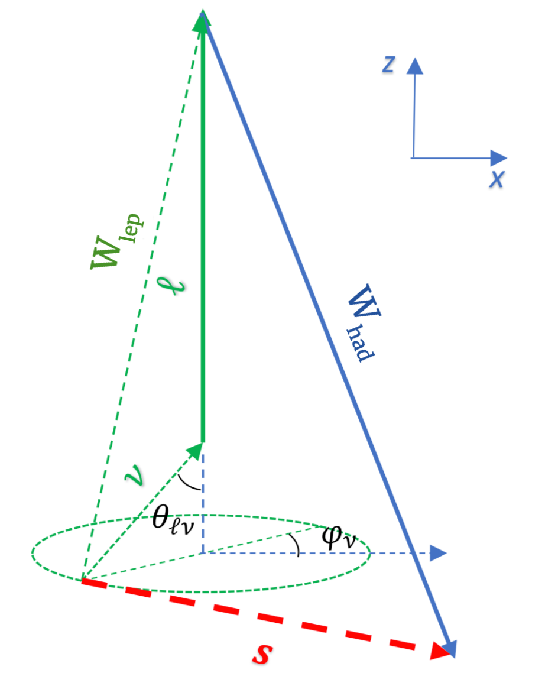
\includegraphics[width = 0.4\textwidth]{Figures/5/minms_coords.pdf}
     \caption{Coordinate system used to evaluate the minimum DH mass \ms that is kinematically required to produce the observed final state, subject to the constraint that \(m_{W_\text{lep}} = 80.4~\GeV\).}
     \label{fig:minms_coords}
  \end{figure}
  
In this rotated coordinate system, the four-momenta \(\mathbf{p}_\nu\), \(\mathbf{p}_\ell\) of the neutrino, lepton and hadronically decaying \(W\) boson, respectively, are given by:

\begin{equation}
\label{eq:neutrino_momentum}
\mathbf{p}_\nu = E_\nu(\sin\theta_{\ell\nu}\cos\phi_\nu, \sin\theta_{\ell\nu}\sin\phi_\nu, \cos\theta_{\ell\nu}, 1)
\end{equation}

\begin{equation}
\label{eq:lepton_momentum}
\mathbf{p}_\ell = E_\ell(1, 0, 0, 1)
\end{equation}

\noindent and 

\begin{equation}
\label{eq:lepton_momentum}
\mathbf{p}_{W_\text{had}} = (E_{W_\text{had}}, p_{W_\text{had}, x}, 0, p_{W_\text{had}, z})
\end{equation}

\noindent where \(\theta_{\ell\nu}\) is the angular separation between the lepton and the neutrino, and \(\phi_\nu\) is the angle of the neutrino relative to the \(x\) axis in the \(xy\) plane. The \ms is then obtained by squaring the four-momenta in Eq. \ref{eq:dh_4momentum}:

\begin{multline}
\label{eq:ms_squared}
\ms^2 = (\mathbf{p}_{W_\text{had}} + \mathbf{p}_{W_\text{lep}})^2 = (\mathbf{p}_{W_\text{had}} + \mathbf{p}_\ell + \mathbf{p}_\nu)^2 \\
= (E_{W_\text{had}} + E_\ell + E_{\nu})^2 - (p_{W_\text{had}, x} + E_{\nu}\sin \theta_{\ell\nu}\cos \phi_{\nu})^2 - (E_{\nu}\sin \theta_{\ell\nu}\sin \phi_{\nu})^2 - (E_\ell + p_{W_\text{had}, z} + E_{\nu}\cos \theta_{\ell\nu})^2
\end{multline}

\noindent It can be shown by taking derivatives of Eq. \ref{eq:ms_squared} that the minimum \ms occurs when \(\phi_v=0\) (i.e. when the neutrino is in the same plane as the \(\mathbf{p}_{W_\text{had}}\)).


Setting \(\phi_v=0\) in Eq. \ref{eq:ms_squared} and using the pythagorean identity \(\sin \theta = \sqrt{1-\cos^2\theta}\):

\begin{multline}
\label{eq:ms_squared_simplified}
m_s^2 = \left(E_\ell + E_\nu + E_{W_\text{had}}\right)^2 - \left(p_{W_\text{had}, x}  + E_\nu\sqrt{1 - \cos^2\theta_{\ell\nu}}\right)^2 \\ - \left(E_\ell + p_{W_\text{had}, z}\cos \theta_{Wl} + E_\nu\cos \theta_{\ell\nu} \right)^2
\end{multline}

This leaves an equation for \ms with two unknowns: the energy \(E_\nu\) of the neutrino, and the cosine \(\cos\theta_{\ell\nu}\) of the angle between the lepton and the neutrino. The neutrino energy is determined independently, by imposing the constraint that the mass \(m_{W_\text{lep}}\) of the leptonically decaying \(W\) boson be set to the on-shell \(W\) boson mass of \(m_W=80.4~\GeV\):

\begin{equation}
\label{eq:Ev}
m_{W_\text{lep}}^2 = m_W = (p_\ell + p_{\nu})^2 = 2p_\ell p_{\nu} = 2E_\ell E_{\nu}(1 - \cos\ \theta_{\ell\nu})\\
\end{equation}

\noindent Solving for \(E_\nu\):

\begin{equation}
\label{eq:Ev_solved}
E_{\nu} = \frac{m_W^2}{2E_\ell(1 - \cos\ \theta_{\ell\nu})}
\end{equation}

With this independent determination of \(E_\nu\), the minimum \ms in Eq. \ref{eq:ms_squared_simplified} is evaluated numerically by scanning over \(\cos\ \theta_{\ell\nu} \in [-1,1]\) and identifying the value of \(\cos\ \theta_{\ell\nu}\) which minimizes \ms (excluding \(\cos\ \theta_{\ell\nu}=1\) to avoid a singularity in Eq. \ref{eq:Ev_solved}).

Figure \ref{fig:minms_reco} shows distributions of the minimized \ms (``\minms") for MC simulated events produced for the DH signal model over a range of \ms (left column) or \mZp (right column). The distributions are more sharply peaked for lower \ms, and for higher \ms the location of peak in \minms becomes increasingly shifted to the left of (i.e. below) the actual modelled \ms. The minimal variation between the different modelled values of \mZp presented in distributions in the right-hand column of Figure \ref{fig:minms_reco}, which scan over a range of \mZp for the same \ms, offers an encouraging indication that the value of the \minms variable is primarily a function of the \ms parameter in the model that it is designed to approximate, and that its dependence on other model parameters is minimal. 

Despite the shifted location of the peaks at higher \ms, the presence of distinct peaks in the approximate vicinity of the modelled \ms imply that the \minms variable can be a valuable tool to aid in discriminating between events in the data that could be consistent with the DH signal process, and SM background processes. For this reason, events in the signal regions are binned in \ms when fitting the ATLAS data to the predicted yields of events produced by the DH signal model and the SM background processes to search for evidence of the DH model in the data in this DM search. The binning in \minms is presented in detail in Section zzz \textcolor{red}{(Note to Bob: will update when section on binning is written)}.

\begin{figure}[H]
	\centering
	\begin{subfigure}[b]{0.49\textwidth}
	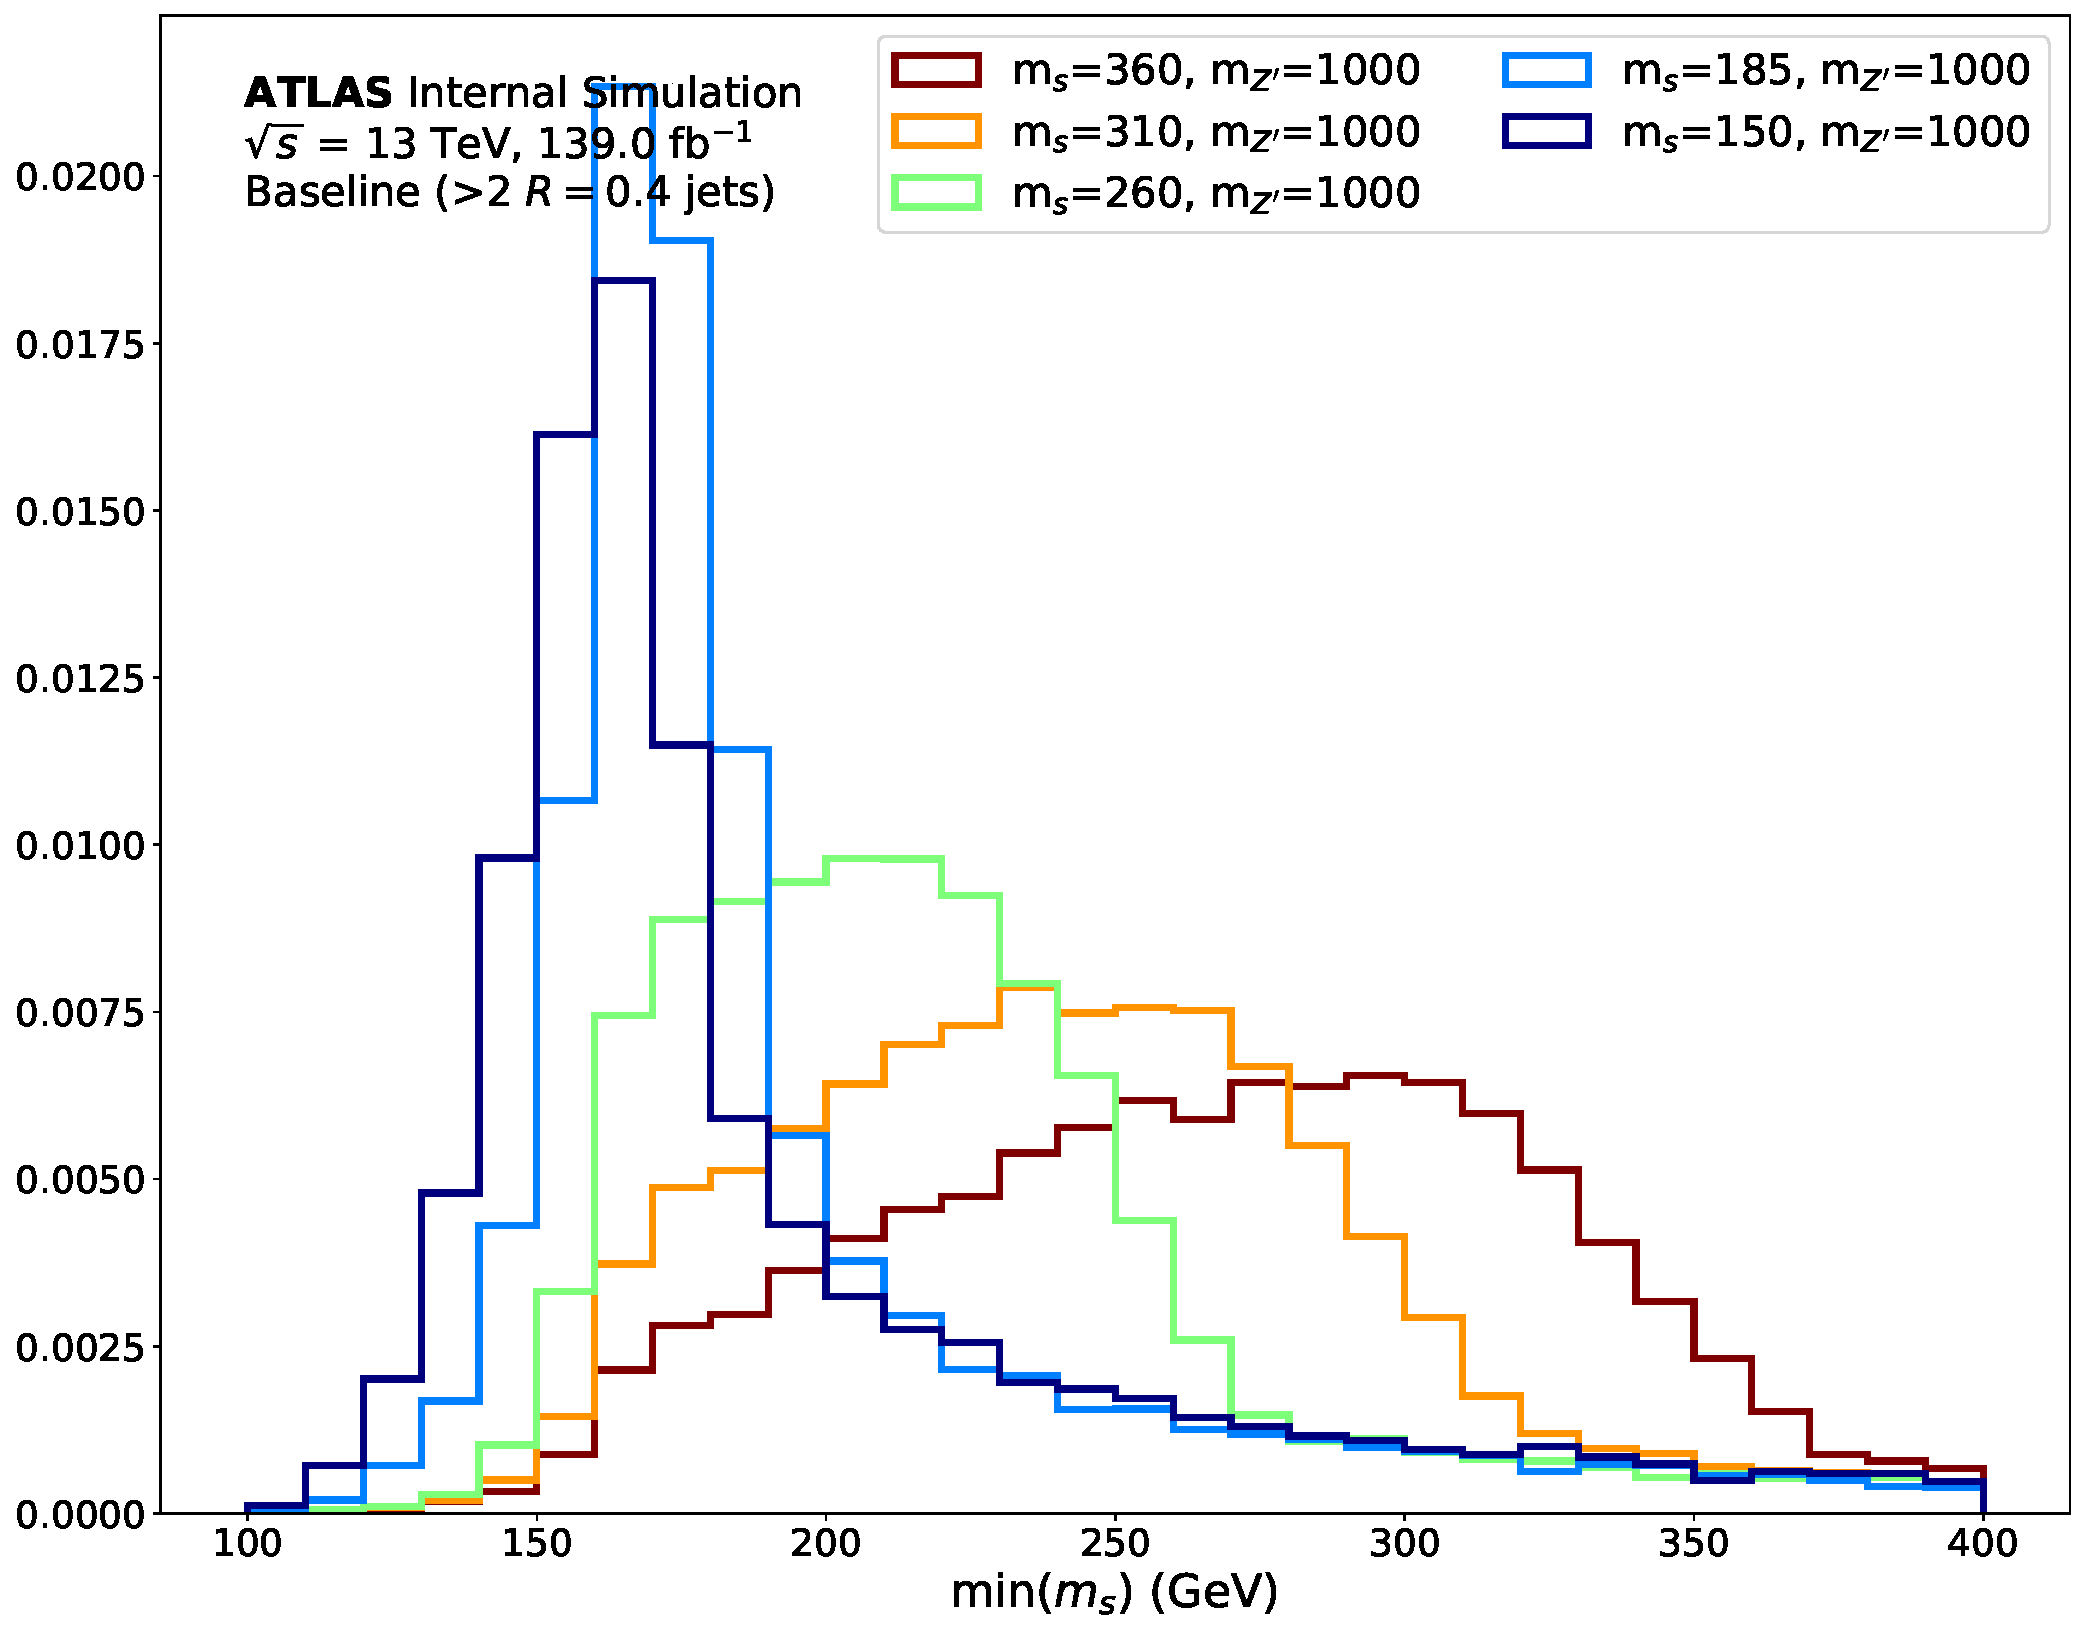
\includegraphics[width=0.95\textwidth]{Figures/5/TARJets10_minmS_res_ms.pdf}
	\caption{\(p_{W_\text{had}}\) reconstructed using \(R=0.4\) \smallR jets (see Section \ref{sec:resolved_w_cand}): \mZp Fixed, \ms Varied}
	\label{fig:minms_res_ms}
	\end{subfigure}
	\begin{subfigure}[b]{0.49\textwidth}
	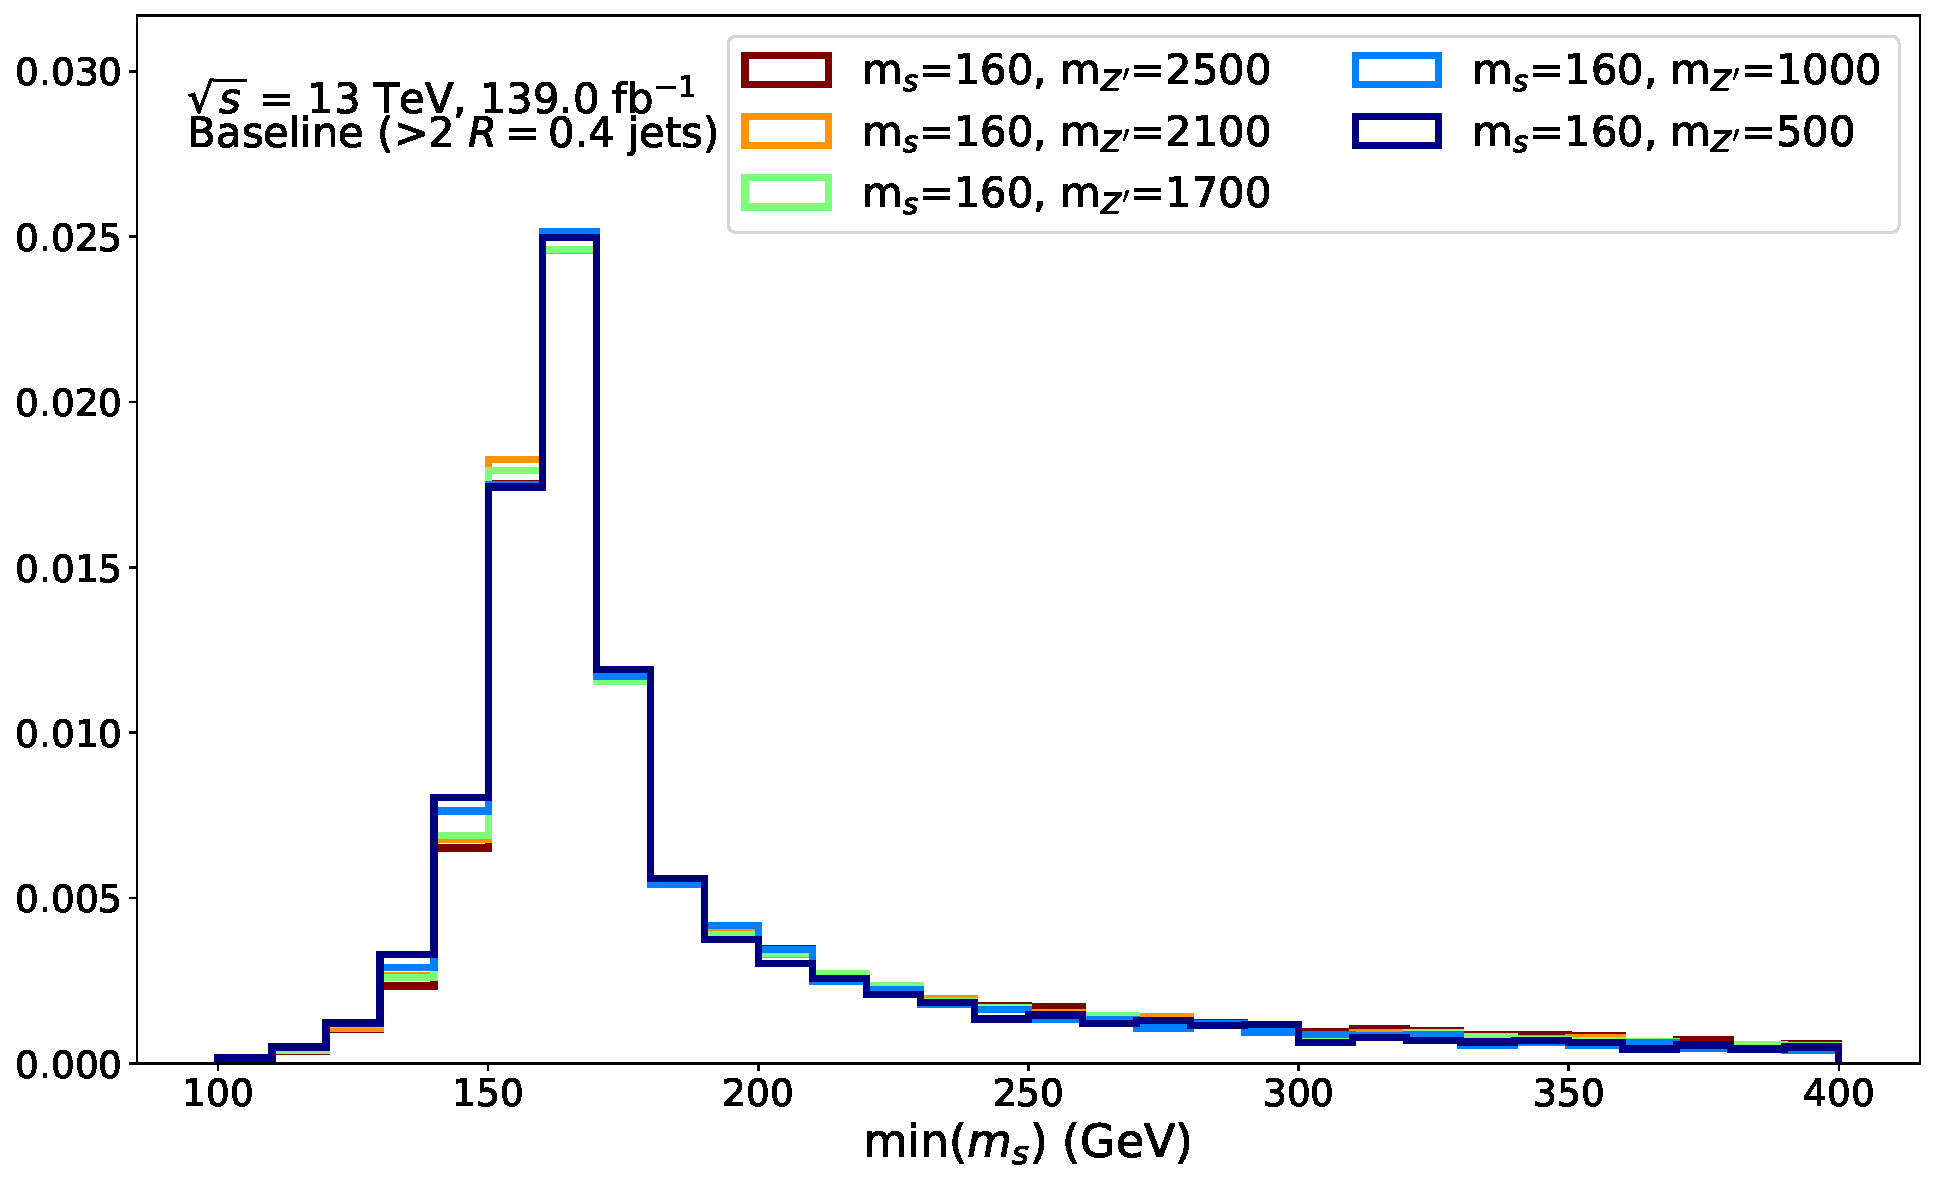
\includegraphics[width=0.95\textwidth]{Figures/5/TARJets10_minmS_res_mZp.pdf}
	\caption{\(p_{W_\text{had}}\) reconstructed using \(R=0.4\) \smallR jets (see Section \ref{sec:resolved_w_cand}): \mZp Fixed, \ms Varied\ms Fixed, \mZp Varied}
	\label{fig:minms_res_mZp}
	\end{subfigure}
	\begin{subfigure}[b]{0.49\textwidth}
	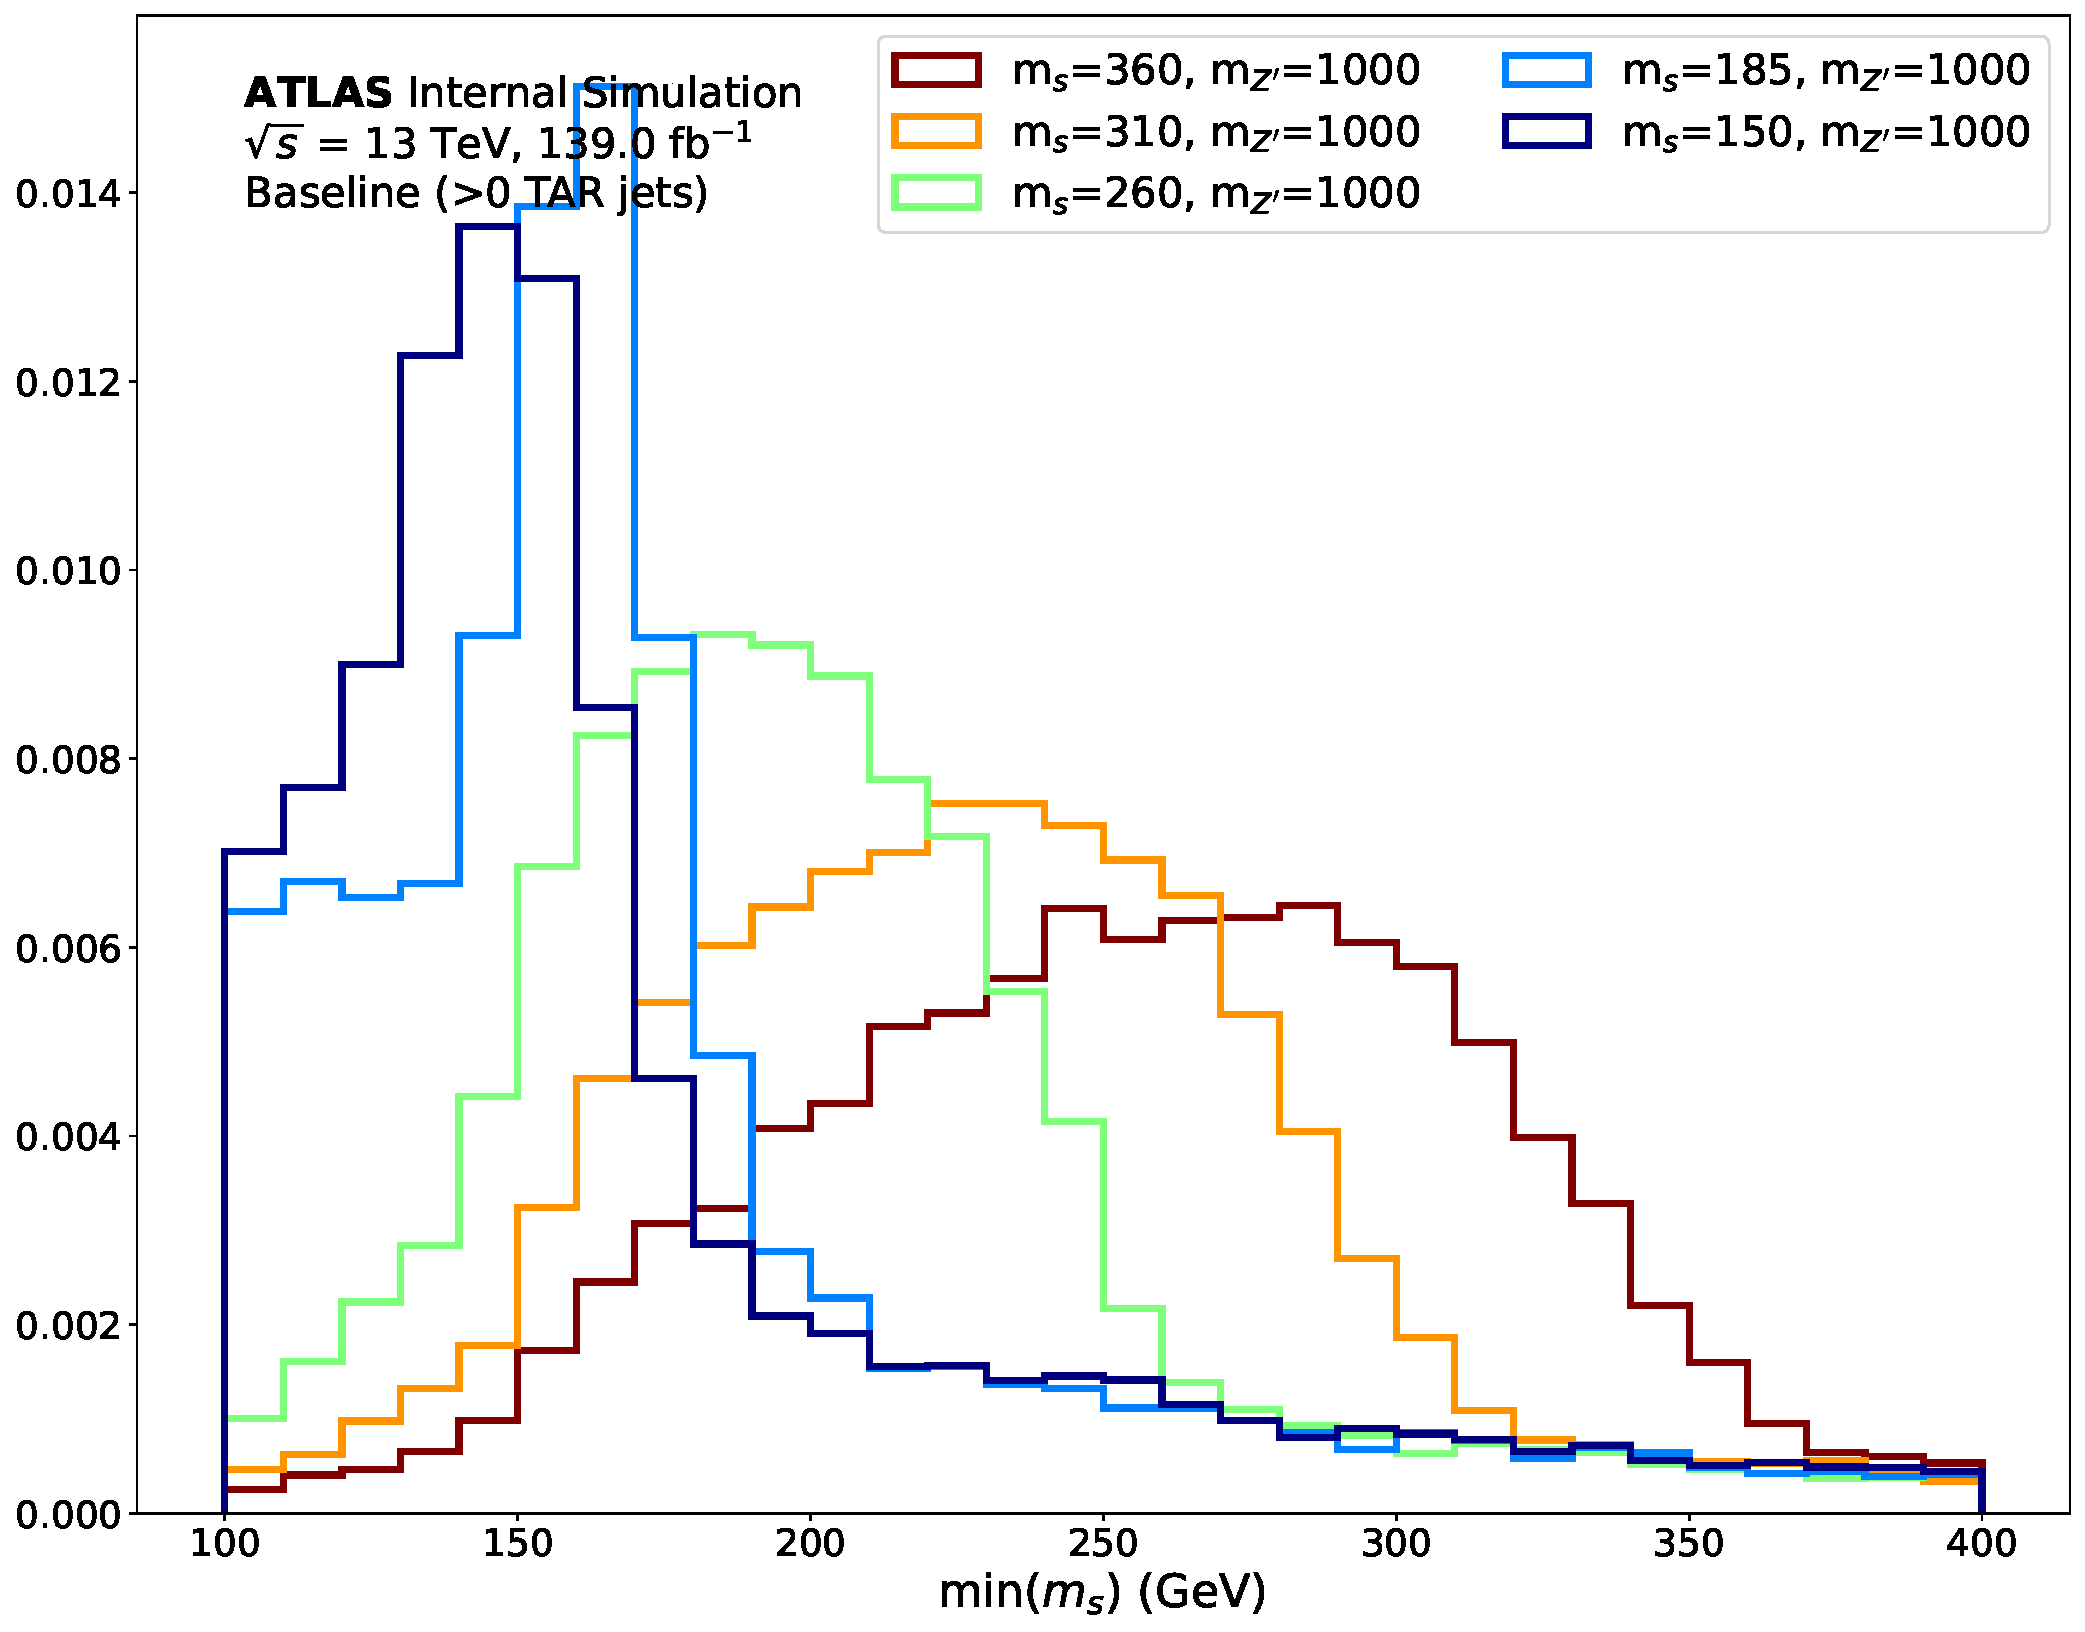
\includegraphics[width=0.95\textwidth]{Figures/5/TARJets10_minmS_mgd_ms.pdf}
	\caption{\(p_{W_\text{had}}\) reconstructed using the leading TAR jet (see Section \ref{sec:TAR_jets}): \mZp Fixed, \ms Varied}
	\label{fig:minms_res_ms}
	\end{subfigure}
	\begin{subfigure}[b]{0.49\textwidth}
	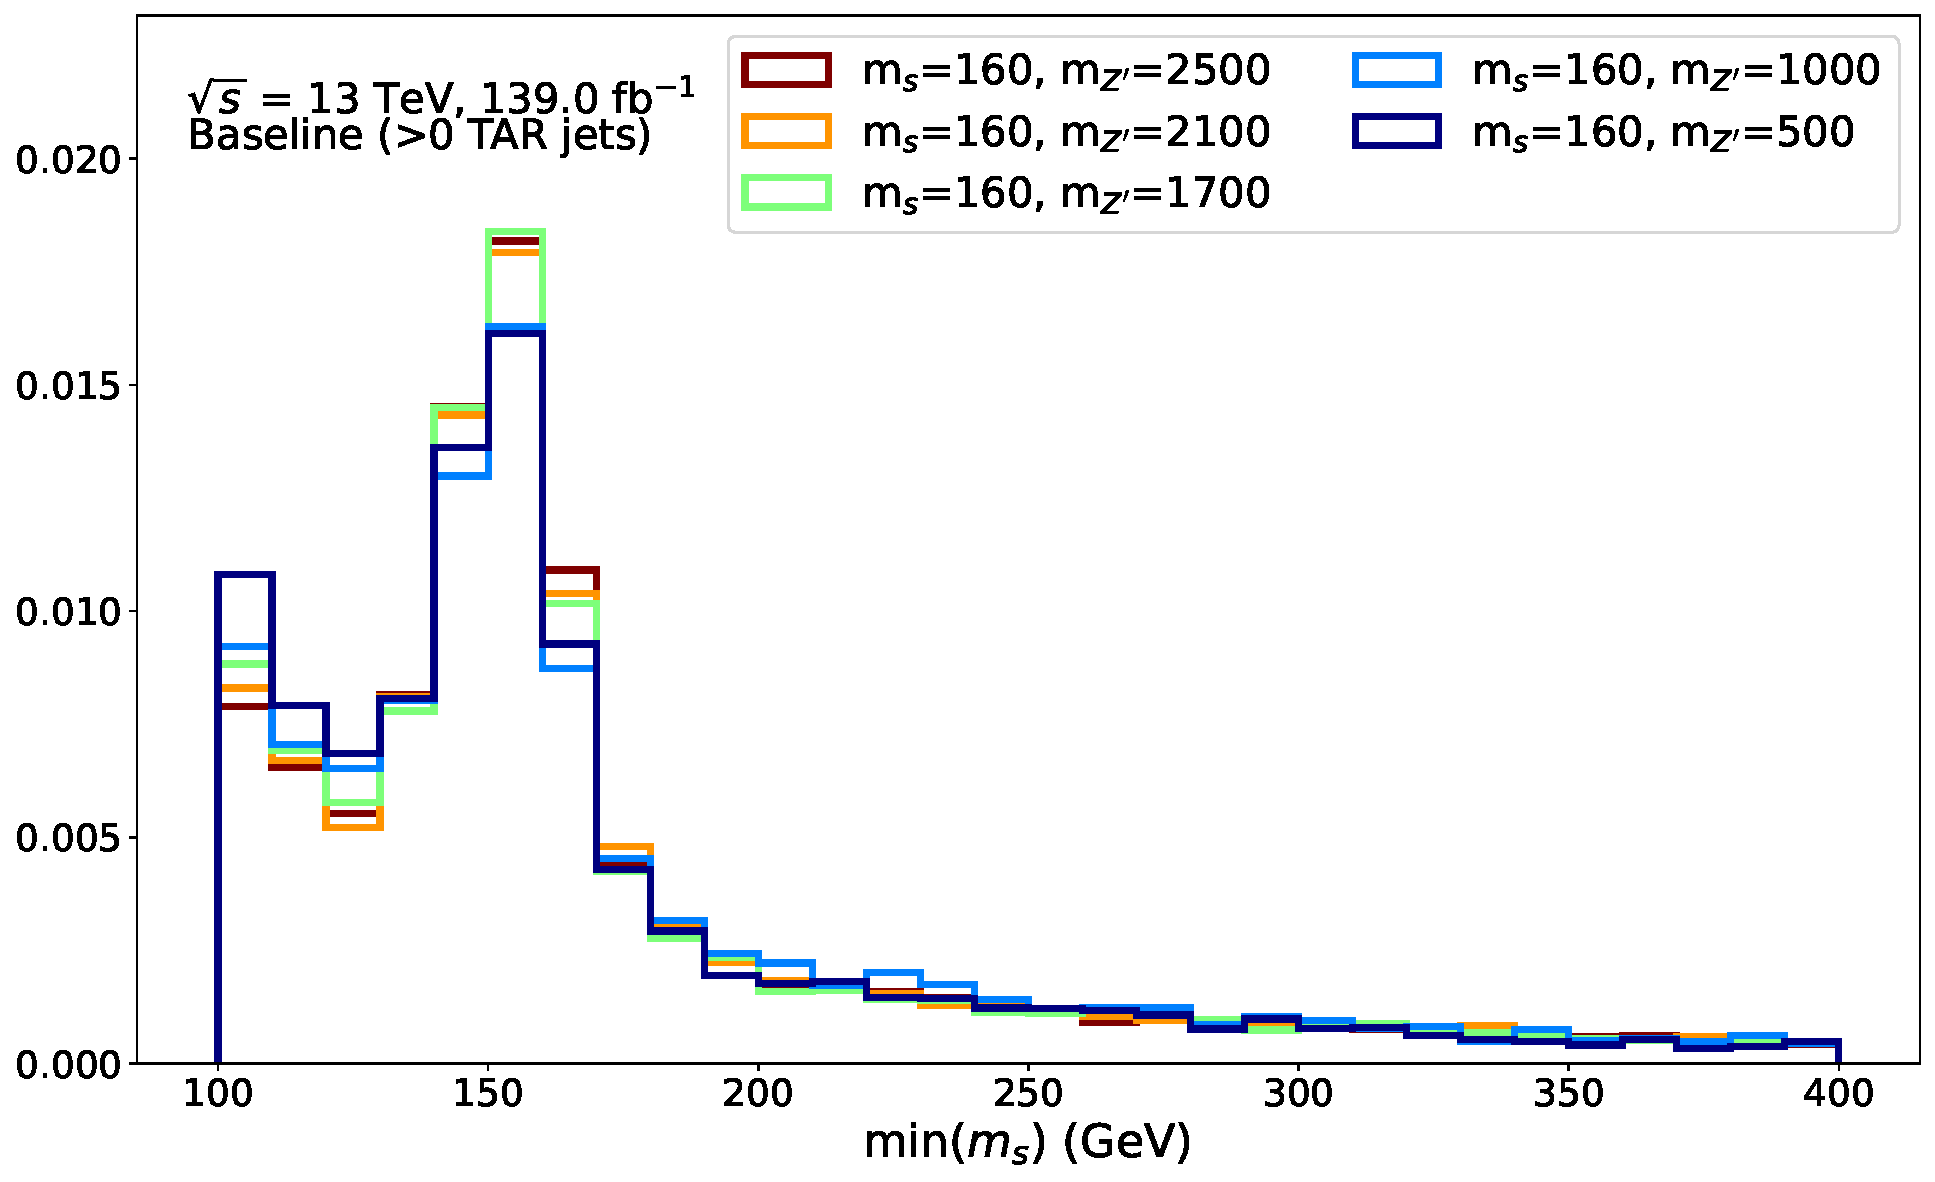
\includegraphics[width=0.95\textwidth]{Figures/5/TARJets10_minmS_mgd_mZp.pdf}
	\caption{\(p_{W_\text{had}}\) reconstructed using the leading TAR jet (see Section \ref{sec:TAR_jets}): \mZp Fixed, \ms Varied\ms Fixed, \mZp Varied}
	\label{fig:minms_res_mZp}
	\end{subfigure}
	\caption[]{Distributions of the candidate \ms, reconstructed using the minimization strategy presented in Section \ref{sec:minms}, for MC simulated events produced for the DH signal model over a range of \ms and \mZp. Distributions are normalized to unit area. Events included in all distributions are required to pass the baseline selection requirements presented in Section \ref{evt_selections}. Events in the top row for which \(p_{W_\text{had}}\) is reconstructed using \(R=0.4\) \smallR jets are required to have at least two \(R=0.4\) \smallR jets reconstructed in the final state, and events in the bottom row for which \(p_{W_\text{had}}\) reconstructed using the leading TAR jet are required to have at least one TAR jet reconstructed in the final state.}
	\label{fig:minms_reco}
\end{figure}

\subsection{Transverse Mass}
\label{sec:transverse_mass}

The transverse mass \(m_T(\met, \ell)\) between the lepton and \met is considered in this search because it is sensitive to the presence of additional \met beyond that arising from the neutrino in the leptonic decay of the \(W_\text{lep}\). It is computed for events measured in the ATLAS detector as:

\begin{equation}
\label{eq:mtlepmet_atlas}
m_T(\ell, \met) = \sqrt{2p_{T, \ell} \met(1-\cos\theta_{\ell, \met})}
\end{equation}


\noindent which comes from the more general transverse mass definition \cite{PDG_kin}

\begin{multline}
\label{eq:mtlepmet_full}
m_{T, \text{ full}}^2(\ell, \met) = (E_{T, \ell}^2 + E_{T, \met}^2 - (p_{T, \ell}^2 + p_{T, \met}^2)) \\
= m_\ell^2+m_{\met}^2 + 2E_{T, \ell}, E_{T, \met}(1-\cos\theta_{\ell, \met})
\end{multline}

\noindent under the assumptions that the masses associated with the lepton and \met are negligibly small compared with their momenta. The assumption of negligible lepton mass is in general justified given the energy of LHC collisions. The assumption of negligible mass associated with \met is justified if the true \met arises only from the neutrino in the leptonic \(W_\text{lep}\) decay, as it would in the leading SM backgrounds. In the signal model, however, there is additional mass associated with the \met arising from DM production. The result, shown in figure \ref{fig:mT_lep_met} after applying the baseline selection, is that the bulk of the SM background has \mtlepmet below the W mass peak, but the signal distribution tends to be peaked closer to \(\sim 250~\GeV\). 

\begin{figure}[H]
	\centering
	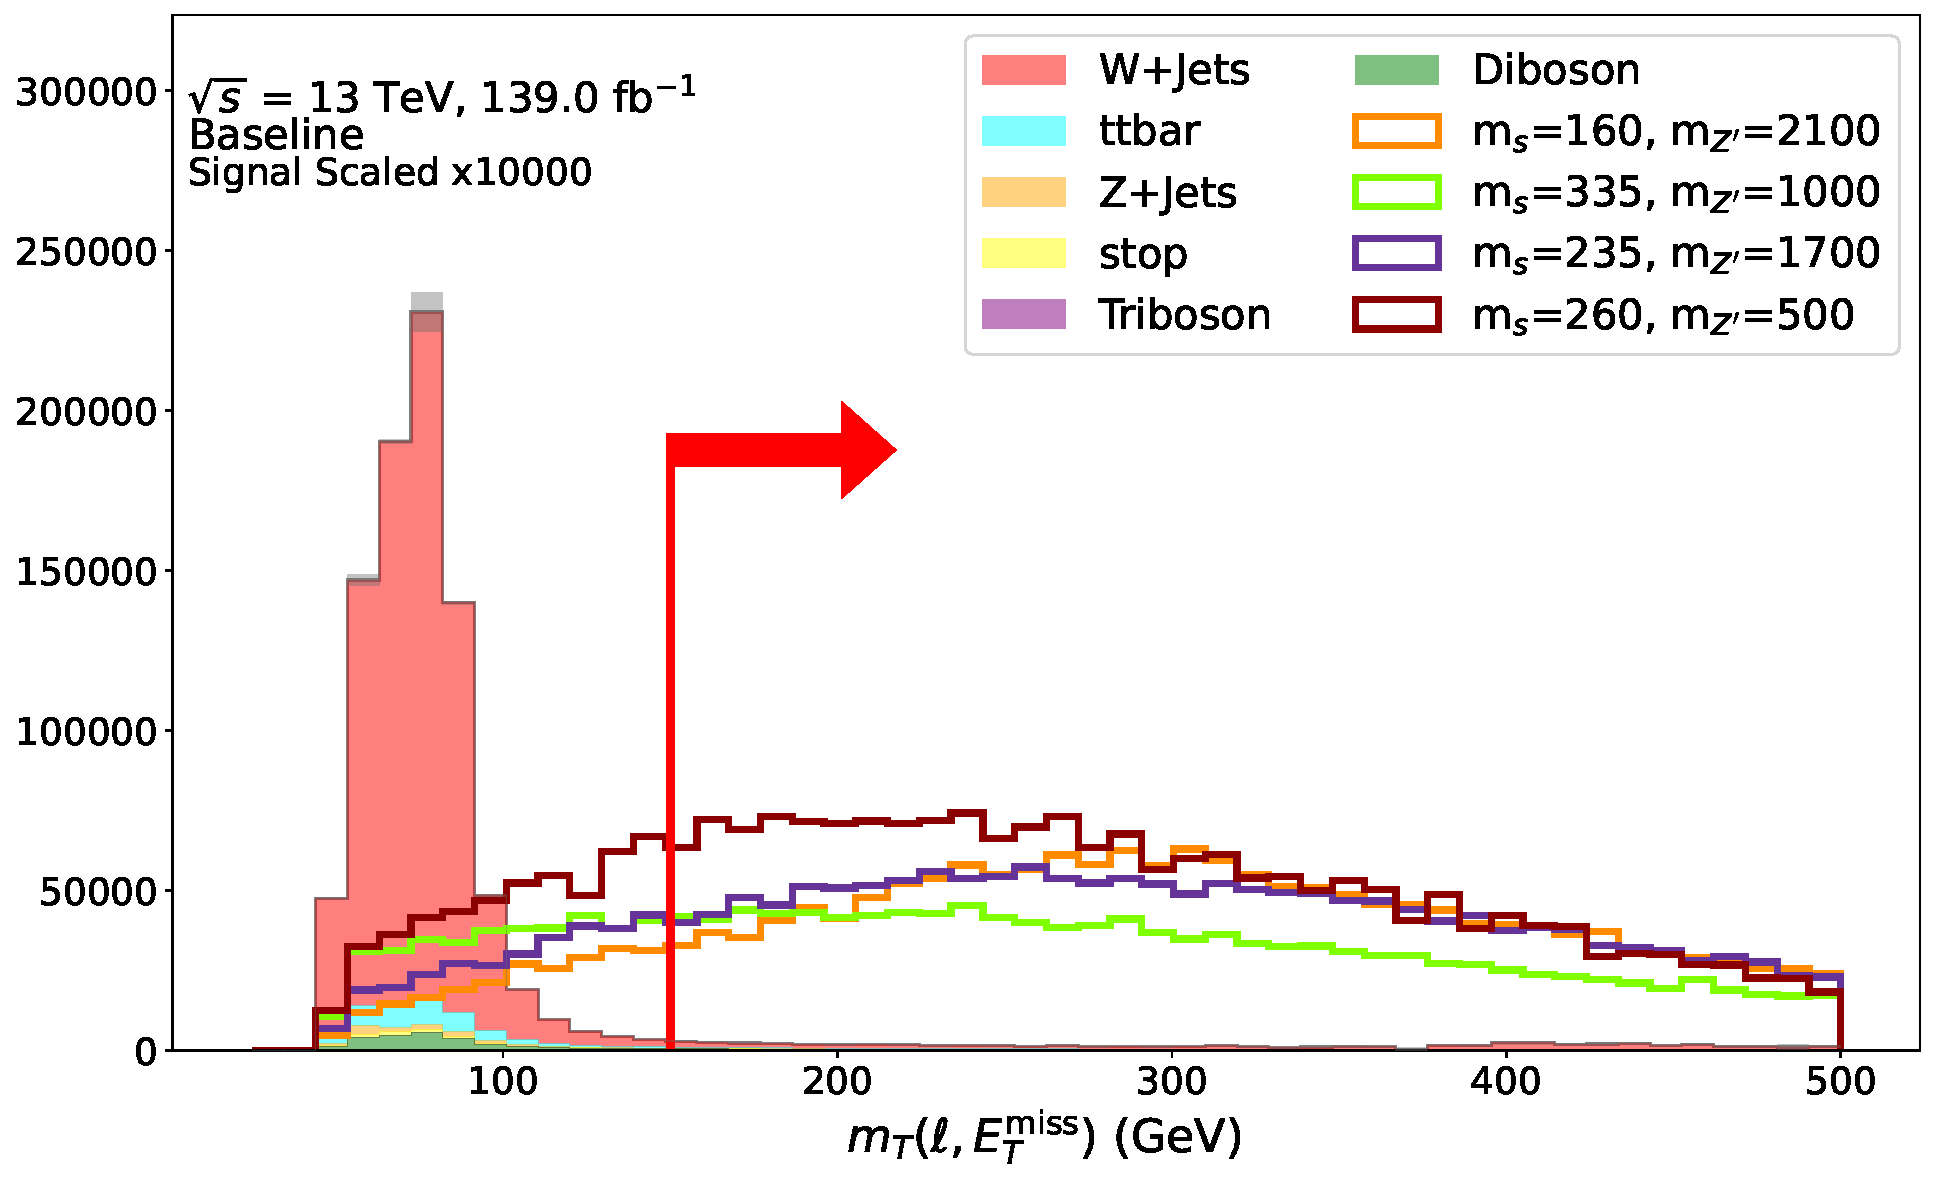
\includegraphics[width=0.7\textwidth]{Figures/5/mT_lep_met_N_1.pdf}
	\caption[]{Transverse mass distribution for SM background and several signal points with baseline selections, excluding the lower bound on \mtlepmet. The lower panel shows the ratio of yields predicted for the signal over the sum of MC background processes. The red line and arrow indicate the placement of the baseline selection on \mtlepmet.}
	\label{fig:mT_lep_met}
\end{figure}

\section{Event Selections}
\label{sec:evt_selections}'

Selections are applied to the ATLAS collision data and MC simulated events with the aim of defining subsets, or ``regions" of data that are enriched in a particular process of interest for the search. The regions are designed and optimized using MC simulated data (see Section \ref{chapter:mc} for a detailed discussion of MC simulation and its application for simulating data produced by the ATLAS detector). The use of MC simulated data makes it possible to quantify the relative contribution to the expected yield of events in the region arising from each physics process.

Selections which define the ``Signal regions" (SRs) are optimized to produce an enriched yield of MC simulated events produced using the DH signal model (referred to as ``signal events"), with a minimal yield of simulated events generated to model SM background processes (referred to as ``background events"). A discrepancy between the ATLAS collision data and the predicted yield of SM backgrounds in the signal regions would be an indication of a new BSM physics process producing a signature in the detector consistent with the signal model. ``Control regions" (CRs) are optimized to have an enriched yield of MC simulated events modelled by one particular SM background process. \wjets and \ttbar CRs are defined for this DM search to obtain a data-driven constraint on the overall normalization of these SM background processes in the signal region. 

\subsection{Kinematic Categories}
\label{sec:kin_categories}

Within each of the signal and control regions, the analysis selection is divided into two kinematic regimes, referred to as ``categories". The ``merged" category is designed to target the merged regime discussed in Section \ref{sec:TAR_jets} in which the hadronic decay products are sufficiently boosted as to be reconstructed as a single \(R=1.0\) TAR jet. The leading \pt TAR jet is then used to reconstruct the candidate hadronically decaying \(W\) boson \(W_\text{had}\) in the signal model. The ``resolved" region targets the low-boost regime in which the hadronic decay products are have sufficient angular separation that they cannot be reclustered into a TAR jet, and are instead reconstructed as resolved \smallR \akt \(R=0.4\) jets, and the \(W_\text{had}\) is reconstructed using the two \smallR jets whose combined invariant mass is closest to \(m_W=80.4~\GeV\).

\Fig{\ref{fig:categories}} illustrates the two kinematic categories.

\begin{figure}[htbp]
	\centering
	\begin{subfigure}[t]{0.45\textwidth}
	\centering
	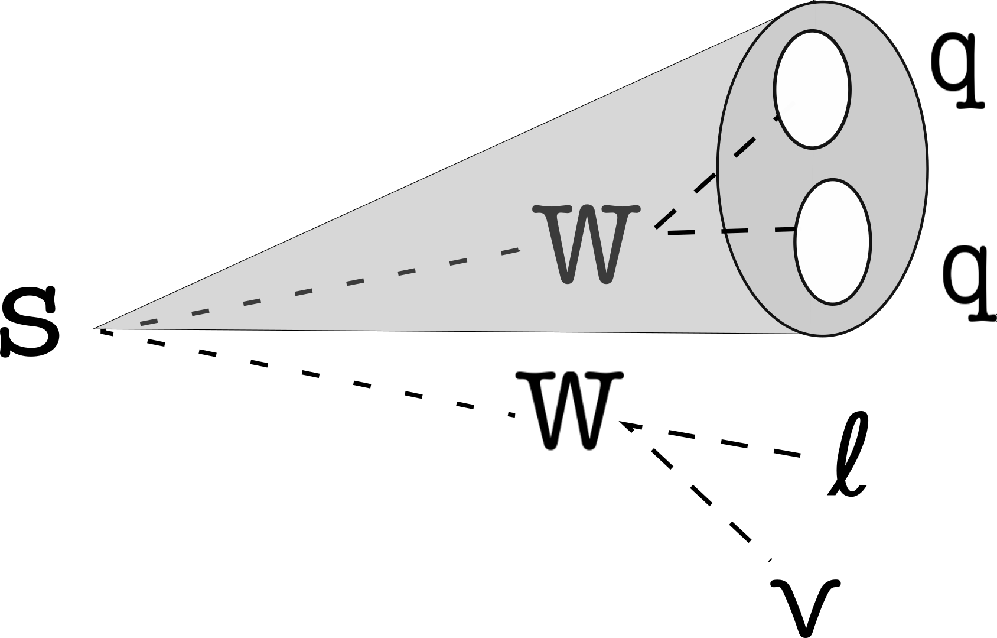
\includegraphics[width=0.75\textwidth]{Figures/5/merged.pdf}
	\end{subfigure}
	\begin{subfigure}[t]{.45\textwidth}
	\centering
	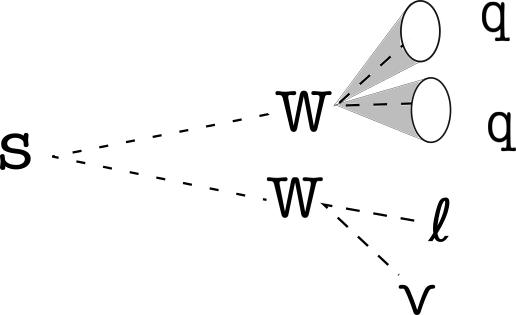
\includegraphics[width=0.75\textwidth]{Figures/5/resolved.png}
	\end{subfigure}
	\caption{A graphical representation of two kinematic categories based on the characteristics of the signal. Left: merged category, in which the jets produced by the \(w\rightarrow q\bar{q}\) are sufficiently boosted as to be reconstructed within a single \largeR TAR jet. Right: \resolved category, in which the two quarks are reconstructed separately as two \smallR \akt \(R=0.4\) jets.}
	\label{fig:categories}
\end{figure}

Within each of the signal and control regions, the selection is divided into the merged and resolved kinematic categories presented in Section \ref{sec:kin_categories}. Events are classified into the merged category if there is at least one reconstructed \(R=1.0\) TAR jet in the final state (\(\NTAR > 0\)), and the resolved category if there are at least two reconstructed \(R=0.4\) \smallR jets (\(\Njets > 1\)). Selections are further refined and optimized separately within each category. It is worth noting that, as is, the requirements for events to be classified into the merged or resolved categories are not mutually exclusive - i.e. there are events which have at least one \(R=1.0\) TAR jet \textbf{and} at least two \smallR jets. To avoid double-counting the same events in the search, orthogonality between the merged and resolved categories is therefore enforced in all of the signal and control regions by explicitly requiring events which pass the requirements to be classified into the resolved category in any region to have additionally failed the merged category selection in all regions.  

\subsection{Baseline selection}
\label{ap:preselection}

The baseline preselection is common to all analysis regions and categories used in the search, and is used to roughly define the region of interest for the search prior to any detailed optimization of selection requirements or sub-division into separate analysis regions. The baseline selection is defined as follows:

\begin{itemize}
\item (1 signal muon or 1 signal electron) and no additional baseline muons or electrons
\item (\met trigger passed) OR ( (single muon trigger passed) AND (signal muon matched to muon trigger) )
\item \(\met > 200~\GeV\)
\item \(\metsig > 5\)
\item \(\mtlepmet > 50~\GeV\)
%\item veto on b-tagged \smallR (\(R=0.4\)) jets (a.k.a. \bjet veto)
\item \(\NTAR > 0\) or \(\Njets > 1\)
\end{itemize}

See Section \ref{sec:charged_leptons} for the definitions of baseline and signal muons and electrons, and Section \ref{sec:triggers_evt_selection} for details of the \met and single muon triggers as well as the single muon trigger matching requirement. The requirement that there be no baseline muons or electrons in addition to the single signal lepton is designed to obtain a higher purity of the single lepton final state predicted by the signal model by vetoing events in which an additional lepton was produced from the hard scatter and reconstructed as a baseline lepton, yet failed the criteria to be identified as a signal lepton. 


\subsection{Signal Region Definition}
\label{sec:sr_selection}

In addition to the baseline selection, a veto on jets identified as having been induced by a \(b\) quark (a.k.a. a \bjet veto) is applied in the SR to reduce the yield of SM \ttbar and single-top processes discussed in Section \ref{sec:SM_bkg_sim}. See Section \ref{sec:btag} for details of the \bjet tagging algorithm. 


Within each category, the baseline selection is further refined by optimizing the exact placements of upper or lower bounds, also referred to as ``cuts", on variables for which the distributions of MC simulated events generated according to the signal model differs appreciably from MC simulated distributions of the SM background processes.

Broadly, the cut placements are optimized to maximize the predicted yield of MC simulated events which model the DH signal process relative to the predicted yield of those which model the SM background processes. However, this basic benchmark fails to account for the fact that, as discussed in Section \ref{sec:mc_intro}, the relative statistical uncertainty associated with the MC simulated yield predictions will increase as the selections are tightened (i.e. lower bounds are increased or upper bounds are reduced) due to the resulting reduction in the number of MC simulated events which pass the selections. As the relative statistical uncertainty of the predicted yields increases, the ability of the search to confidently identify an excess of ATLAS collision events above the predicted yield of SM background processes - which would be indicative of additional events produced by a BSM process - is reduced. Furthermore, as the predicted yield of events is reduced, the relative statistical uncertainty associated with the number of observed events, derived from the Poisson distribution, will also increase and impact the sensitivity of the search. Therefore, while if is often valuable to tighten certain selections in order to increase the relative predicted yield of the signal process, it is also important to avoid over-tightening them to the point that the statistical uncertainty of the predicted and observed event yields begins to reduce the sensitivity of the search. 

A metric known as the ``Asimov discovery significance" \cite{Buttinger:2643488} \(Z\) is used as a means of quantifying the sensitivity of a search given the predicted yields \(s\) and \(b\) of the signal and background processes, respectively, while also accounting for the statistical uncertainty \(\sigma_b\) associated with the MC simulation used to obtain the predicted background yield:

\begin{equation}
  \label{eq:asimov}
  Z(s, b, \sigma_b) = \left[ 2(s+b)\left(
    \ln\left[ \frac{(s+b)(b+\sigma_b^2)}{b^2 + (s+b)\sigma_b^2} \right]
    - \frac{b^2}{\sigma_b^2}\ln\left[ 1 + \frac{\sigma_b^2 s}{b(b+\sigma_b^2)} \right]
  \right) \right]^\frac{1}{2}
\end{equation}

\subsubsection{Optimization Strategy for Signal Region Definition}
\label{sec:sr_opt}

After applying the baseline selections and \bjet veto, the placement of upper and lower bounds is optimized for the selection variables listed in Table \ref{tab:opt_vars}. The choice of selection variables was made based on a visual assessment of the impact of cuts on all the variables considered as candidate selection variables on the Asimov discovery significance \(Z\). Visualization of \(Z\) with respect to the cut placement on each variable is done using so-called ``N-1" plots, which are shown for the finalized selections in the merged and resolved signal regions, respectively, in Figures \ref{zzz} and \ref{zzz}. The N-1 plots are produced for a given variable \(v\) and a given set of candidate selections on all other variables as follows:

\begin{itemize} 
\item Place the candidate selections on all variables except for the variable \(v\).
\item In the upper panel, plot the distributions of the background and signal processes, binned in the variable \(v\).
\item In the lower panel, plot the distributions of the Asimov discovery significance \(Z\) for each signal process plotted in the upper panel.
\item If comparing the placement of an \textbf{upper bound} \(v_u\) on the variable \(v\): calculate the Asimov significance \(Z(v_u)\) for all events with \(v<v_u\): 

\begin{equation}
\label{eq:asimov_upper}
\begin{gathered}
s_u = \sum_{i \in \{\text{signal}, v(i) < v_u\}} w(i) \\
b_u =  \sum_{i \in \{\text{SM backgrounds}, v(i) < v_u\}} w(i) \\
\sigma_{b_u} = \sqrt{ \sum_{i \in \{\text{SM backgrounds}, v(i) < v_u\}} \big[w(i)\big]^2 } \\
Z(v_u) = Z(s_u, b_u, \sigma_{b_u})
\end{gathered}
\end{equation}

\noindent where each event \(i\) is implicitly required to have passed all the other candidate selections for the given process (signal or SM backgrounds) in addition to \((v < v_u)\), and \(w(i)\) is the event weight associated with event \(i\) (see discussion of event weights in Section \ref{sec:evt_weights}). The statistical variance \((\sigma_b)^2\) is evaluated in Eq. \ref{eq:asimov_upper} as the sum of squared weights for events in the background process which pass all other candidate selections in addition to \((v < v_u)\). 

\item Conversely, if comparing the placement of a \textbf{lower bound} \(v_d\): calculate the Asimov significance \(Z(v_d)\) for all events with \(v>v_d\) by replacing ``\(v<v_u\)" in Eq. \ref{eq:asimov_upper} with ``\(v>v_d\)".
\end{itemize}

The optimization was performed first in the merged category of the SR, with the additional requirement of at least one \(R=1.0\) TAR jet. Once the selections defining the merged SR were finalized, optimization was subsequently performed in the resolved category, with the \(\NTAR > 0\) requirement replaced by \(\Njets > 1\) in addition to a veto on any events which pass the finalized merged SR selections. 

Since the optimal placement of selections was found to vary to some extent for MC simulated data sets with different \ms and \mZp, the cut placements were initially optimized with the aim of maximizing the average Asimov discovery significance for MC simulated data sets at the following four mass points which cover most of the \ms range considered in the search: (\ms, \mZp) = \{(210, 2100), (285, 1700), (310, 500), (335, 1000)\} GeV. The \mZp values of these four mass points were chosen such that the points were near the edge of the so-called ``exclusion range", which represents the range of \ms and \mZp within which the search was expected to be sensitive to the presence (or absence) of events produced by the DH signal model in the ATLAS data, at a 95\% confidence level on the basis of sensitivity studies discussed in Section zzz \textcolor{red}{(Note to Bob: will update when section on sensitivity projections is written)}. It is particularly desirable to optimize the selections at points near the edge of the exclusion range because 

An iterative approach was used to optimize the cut placements at the four signal points which combined:

\begin{itemize}
\item repeated grid searches which scanned over \(1,000,000\) candidate multi-dimensional combinations of cut placements on some or all of the optimized variables to identify combinations which maximized \(Z\), and 
\item visual analysis of N-1 plots such as those shown in Figures \ref{zzz} and \ref{zzz} to visually validate the optimal placements found by the grid searches.
\end{itemize}

It is worth noting that, inspecting Eq. \ref{eq:asimov}, the Asimov discovery significance does not account for the statistical uncertainty \(\sigma_s\) arising from limited MC simulated events in the signal sample. Therefore, in order to ensure sufficient signal region that there were sufficient events in the signal samples, the grid search included an option to avoid cut combinations which reduced the predicted signal yield below some acceptable minimum set by the user. After some testing, it was found that setting a minimum acceptable predicted yield of 15 for the signal point \((\ms, \mZp)=(210, 2100)~\GeV\) was adequate to ensure that the signal samples of interest for cut optimization had a sufficient number of events as to prevent their statistical uncertainty from becoming appreciable compared with other sources of uncertainty. The signal point \((\ms, \mZp)=(210, 2100)~\GeV\) was chosen to define the minimum yield because it was among the signal points in the signal grid with the lowest predicted yield at the time of optimization.

After 

\begin{table}[hp]
\centering
\caption{List of selection variables, with descriptions, for which the placements of cuts were optimized when designing the merged and resolved signal regions. The third and fourth columns indicate whether the variable is used in the merged category, the resolved category, or both.}
\label{tab:opt_vars}
\footnotesize{
\begin{tabular}{l p{6cm} l l }
\toprule
\textbf{Variable} & \textbf{Description} & \textbf{Merged} & \textbf{Resolved} \\
\midrule
\midrule
\met & A \textbf{lower bound} is placed on \met to select for the production of undetected energetic particles. & \checkmark & \checkmark \\
\midrule
\metsig & A \textbf{lower bound} is placed on \metsig to select for a high likelihood that the measured \met arises from undetected particles rather than limited detector resolution. & \checkmark & \checkmark \\
\midrule
\mTAR & Reconstructed mass of the highest-\pt \(R=1.0\) TAR jet. A \textbf{window cut} around the \(W\) boson mass of \(80.4~\GeV\) is placed on \mTAR around the \(W\) to select for events in which the highest-\pt \(R=1.0\) TAR jet actually reconstructs the hadronic decay of a boosted \(W\) boson, rather than other potential sources of strongly interacting particles.  & \checkmark & \(\times\) \\
\midrule
\DtwoTAR & Energy correlation function of the highest-\pt \(R=1.0\) TAR jet. Used to quantify the likelihood that the TAR jet has a two-pronged substructure using the angular separation and transverse momenta of combinations of the jet constituents \cite{Larkoski:2013eya}. & \checkmark & \(\times\) \\
\midrule
\dRTARl & Angular separation in \(\eta\times\phi\) space between the TAR jet and lepton. & \checkmark & \(\times\) \\
\midrule
\Wcandpt & \pt of the reconstructed \(W\) candidate in the resolved regime. & \(\times\) & \checkmark \\
\midrule
\Wcandm & Mass of the reconstructed \(W\) candidate in the resolved regime. & \(\times\) & \checkmark \\
\midrule
\dRWl & Angular separation in \(\eta\times\phi\) space between the reconstructed \(W\) candidate and lepton in the resolved regime. & \(\times\) & \checkmark \\
\midrule
\end{tabular}}
\end{table}


\begin{itemize}

\item Signal region
\begin{itemize}
\item Prioritize optimization of signal points near the edge of expected search sensitivity. 
\item Keep signal region blind during optimization to avoid biasing selection.
\item Introduce variables used for event selection. Distinguish between variables that are optimized (eg. \mtlepmet) vs. fixed (eg. 1-lepton requirement) during optimization.
\item Present concept and implementation of signal region optimization strategy.
\item High-level discussion of why we define CRs to constrain normalizations of dominant \wjets and \ttbar backgrounds.
\end{itemize}

\item CRs
\begin{itemize}
\item Provides data-driven normalization constraint which can be extrapolated to the signal region (more details on extrapolation procedure in Chapter 7)
\item Reduces the impact of (and reliance on) theoretical uncertainties involved in simulating the correct normalizations for these backgrounds. Emphasize the difficulty involved with assigning reliable theoretical uncertainties, and hence the value of using data-driven constraints.
\end{itemize}

\item Summary of design goals for control region
\begin{itemize}
\item High purity of background of interest.
\item Orthogonal to SR.
\item Phase space kinematically similar to SR.
\item Signal contamination negligible compared with uncertainty of total background yield.
\end{itemize}

\item Present the \wjets control region, and motivate the \dR reversal used to define it.
\item Present the \ttbar control region, and motivate the \bjet veto reversal used to define it.
\item Present the additional modifications that were needed in the \merged category to optimize the CR definitions
\begin{itemize}
\item Reducing the lower bound on \metsig to boost stats.
\item Increasing the lower bound on \dR in the \wjets CR to reduce the signal contamination to an acceptable level.
\end{itemize}
\begin{itemize}
\item Summary of all analysis regions.
\end{itemize}
\end{itemize}

\section{Triggers}
\label{sec:triggers_evt_selection}

As described in Section \ref{sec:trigger}, the ATLAS trigger system only saves collision events during data collection which pass both the hardware-based level-1 (L1) trigger and the software-based high-level trigger (HLT). The L1 trigger and the HLT are each comprised of numerous sets of selection criteria, which are also referred to as triggers. Any collision event which satisfies at least one of the triggers which comprise the L1 trigger is processed by the HLT, and likewise if the event satisfies any of the triggers which comprise the HLT it will be kept for later analysis.

The search presented in this thesis is interested in events which produce a single energetic lepton due to the \(s\rightarrow WW(q\bar{q}\ell\nu)\) decay, in addition to high \met due to both the undetected boosted DM in the final state and the undetected \(\nu\) from the \(W\rightarrow \ell\nu\) decay. It is important to determine the efficiency with which the ATLAS trigger system accepts events in the region of phase space defined by the event selections described in Section \ref{sec:evt_selections} above. The efficiency quantifies the probability that an event that the triggers are designed to accept successfully passes the trigger criteria and gets accepted. If the trigger efficiency is \(<100\%\) in any area of the phase space considered in the analysis, it is in general necessary to apply scale factors to any MC simulated events which fall into this phase space to account for the fact some events would have been rejected by the trigger during actual data-taking. It is also then necessary to evaluate and propagate uncertainties associated with these scale factors.

To simplify the trigger efficiency analysis and determine whether any scale factors may be needed, it is helpful to identify a minimal list of triggers which all events considered in the analysis would be expected to pass. One of the event selection criteria for the analysis, presented in Section \ref{sec:evt_selections}, requires all events to have \(\met > 200 \GeV\). Since the ATLAS \met trigger, described in Refs. \cite{met_trigger_performance_2020} and \cite{met_performance_2019}, is designed to efficiently select events with \(\met>150~\GeV\), it is reasonable to expect events which pass the event selection criteria to have also passed the \met trigger with a high efficiency. The specific \met triggers in the ATLAS trigger menu which are considered in this study are chosen following ATLAS recommendations, and vary between different data collection periods defined by ATLAS. The full list of \met triggers used, along with the associated data collection period for each, is listed in Table \ref{tab:summary_triggers_used}.

\begin{table}[ht]
\caption{Summary table of \met triggers from the ATLAS trigger menu used for the search, along with the associated data collection period for each trigger.}
\label{tab:summary_triggers_used}
\footnotesize{
	\begin{center}
	\begin{tabular}{l l }
		\toprule
			Period & MET Trigger \\
			\midrule
			\midrule
			2015 & \textsc{HLT\_xe70\_mht} \\
			\midrule
			2016 (A-D3) & \textsc{HLT\_xe90\_mht\_L1XE50} \\
			\midrule
			2016 (D4-F1) & \textsc{HLT\_xe100\_mht\_L1XE50} \\
			\midrule
			2016 (F2-) & \textsc{HLT\_xe110\_mht\_L1XE50} \\
			\midrule
			2017 (B-D5) & \textsc{HLT\_xe110\_pufit\_L1XE55} \\
			\midrule
			2017 (D6-K) & \textsc{HLT\_xe110\_pufit\_L1XE50} \\
			\midrule
			2018 (B-C5) & \textsc{HLT\_xe110\_pufit\_xe70\_L1XE50} \\
			\midrule
			2018 (C5-) & \textsc{HLT\_xe110\_pufit\_xe65\_L1XE50} \\
		\bottomrule
	\end{tabular}
	\end{center}
	}
\end{table}

The ATLAS trigger system also includes single-muon and single-electron triggers, which are designed to pass events in which a single muon (electron) is reconstructed in the final state which satisfies some minimum \pt requirement. Since the final state considered in the search requires a single charged lepton in the final state, events passing the event selection would also be expected to pass these charged lepton triggers with high efficiency. The specific single muon and electron triggers considered in this study, along with the ATLAS data-taking period(s) in which they were applied, along with the minimum lepton \pt requirement associated with each trigger, are listed in Tables \ref{tab:summary_muon_triggers_used} and \ref{tab:summary_electron_triggers_used}, respectively.

\begin{table}[ht]
\caption{Summary table of single muon triggers from the ATLAS trigger menu used for the search, along with the associated data collection period for each trigger. The minimum muon \pt threshold of each trigger is also listed.}
\label{tab:summary_muon_triggers_used}
\footnotesize{
	\begin{center}
	\begin{tabular}{l l l }
		\toprule
			Periods & Single Muon Trigger & Muon \pt threshold \\
			\midrule
			\midrule
			2015 & \textsc{HLT\_mu20\_iloose\_L1MU15} & 20 \GeV \\
			\midrule
			2016 (A, B-D3, D4-E, F-G2, G3-I3, I4-), & \multirow{3}{*}{\textsc{HLT\_mu50}} & \multirow{3}{*}{50 \GeV} \\
			2017 (B-), & & \\
			2018 & & \\
			\midrule
			2016 & \textsc{HLT\_mu24\_iloose} & 24 \GeV \\
			\midrule
			2015, & \multirow{2}{*}{\textsc{HLT\_mu40}} & \multirow{2}{*}{40 \GeV} \\
			2016 (A) & & \\
			\midrule
			2016 (B-D3, D4-E) & \textsc{HLT\_mu24\_ivarmedium} & 24 \GeV \\
			\midrule
			2016 (D4-E, F-G2, G3-I3, I4-),  & \multirow{3}{*}{\textsc{HLT\_mu26\_ivarmedium}} & \multirow{3}{*}{26 \GeV} \\
			2017 (B-), \\
			2018 \\
		\bottomrule
	\end{tabular}
	\end{center}
	}
\end{table}

\begin{table}[ht]
\caption{Summary table of single electron triggers from the ATLAS trigger menu used for the study presented in Section \ref{sec:triggers_evt_selection}, along with the associated data collection period for each trigger. The minimum electron \pt threshold of each trigger is also listed.}
\label{tab:summary_electron_triggers_used}
\footnotesize{
	\begin{center}
	\begin{tabular}{l l l }
		\toprule
			Periods & Single Muon Trigger & Electron \pt threshold \\
			\midrule
			\midrule
			2015 & \textsc{HLT\_e24\_lhmedium\_L1EM20VH} & 24 \GeV \\
			\midrule
			2015 & \textsc{HLT\_e60\_lhmedium} & 60 \GeV \\
			\midrule
			2015 & \textsc{HLT\_e120\_lhloose} & 120 \GeV \\
			\midrule
			2016 (A, B-D3) & \textsc{HLT\_e24\_lhtight\_nod0\_ivarloose} & 24 \GeV \\
			\midrule
			2016 (A, B-D3, D4-F, G-), & \multirow{3}{*}{\textsc{HLT\_e60\_lhmedium\_nod0}} & \multirow{3}{*}{60 \GeV} \\
			2017 (B-), & & \\
			2018 & & \\
			\midrule
			2016 (A, B-D3, D4-F, G-)  & \textsc{HLT\_e60\_medium} & 60 \GeV \\
			\midrule
			2016 (A, B-D3, D4-F, G-),  & \multirow{3}{*}{\textsc{HLT\_e300\_etcut}} & \multirow{3}{*}{300 \GeV} \\
			2017 (B-), & & \\
			2018 \\
			\midrule
			2016 (A, B-D3, D4-F, G-), & \multirow{3}{*}{\textsc{HLT\_e140\_lhloose\_nod0}} & \multirow{3}{*}{140 \GeV} \\
			2017 (B-), & & \\
			2018 & & \\
			\midrule
			2016 (D4-F, G-), & \multirow{3}{*}{\textsc{HLT\_e26\_lhtight\_nod0\_ivarloose}} & \multirow{3}{*}{26 \GeV} \\
			2017 (B-) & & \\
			2018 & & \\
		\bottomrule
	\end{tabular}
	\end{center}
	}
\end{table}

The lepton triggers are known to be \(<100\%\) efficient, but the resulting scale factors and associated systematic uncertainties are in general well calibrated by dedicated measurements performed within the ATLAS collaboration. As a result, the charged lepton triggers are useful as a means of independently quantifying the efficiency of the \met trigger, as will be shown in a moment, but if the \met trigger can be shown to pass selected events with 100\% efficiency then it is desirable to simply require all selected events to have passed the \met trigger in order to avoid any application of scaling factors and evaluation of related uncertainties.

The efficiency of the \met trigger for a set of event selection criteria which define a given region ``X" is defined equivalently for ATLAS data (``data") and MC simulated events (``MC"). Events considered for the calculation of trigger efficiency are also required to have passed the single lepton trigger (defined as the logical OR of the single muon trigger and the single electron trigger), to independently ensure that all data events considered passed a trigger which is relevant to the final state of interest. The trigger efficiency is given by:

\begin{equation}
\label{eq:met_trig_eff}
\begin{footnotesize}
\text{eff}_\text{\met, region X} = \frac{\sum_i w_i\text{ passing (\met triggers)\&(single lepton triggers)\&(selection cuts for region X)}}{\sum_i w_i\text{ passing (single lepton triggers)\text{ AND }(selection cuts for region X)}}
\end{footnotesize}
\end{equation}

\noindent where $w_i$ is the total event weight for event \(i\) ($w_i=1$ in the case of data). See Section \ref{sec:evt_wts} for a detailed discussion of weights that are assigned to the MC simulated events. Correction scale factors, dependent on the \pt and \(\eta\) of the final-state lepton in each event, are included in the MC event weights in Eq. \ref{eq:met_trig_eff} to account for the \(<100\%\) trigger efficiency of the single lepton triggers. 

Figure \ref{fig:mettrig} compares the \met trigger efficiency defined in Eq. \ref{eq:met_trig_eff} for MC simulated events and ATLAS data for the region defined with the baseline selections, with the following modifications:

\begin{itemize}
\item The \metsig cut is loosened to \(\metsig>5\) and the \mtlepmet cut is loosened to \(\mtlepmet > 100~\GeV\) to enhance statistics.
\item A range of lower bounds on the \met are considered, from \(\sim100~\GeV\) to \(\sim500~\GeV\).
\item The single charged lepton is required to be an electron (a.k.a. the ``electron channel") in Figure \ref{fig:mettrig_e} and a muon (a.k.a. the ``muon channel") in Figure \ref{fig:mettrig_mu}.
\end{itemize}

\begin{figure}[htbp]
  \centering
     \begin{subfigure}{0.49\textwidth}
     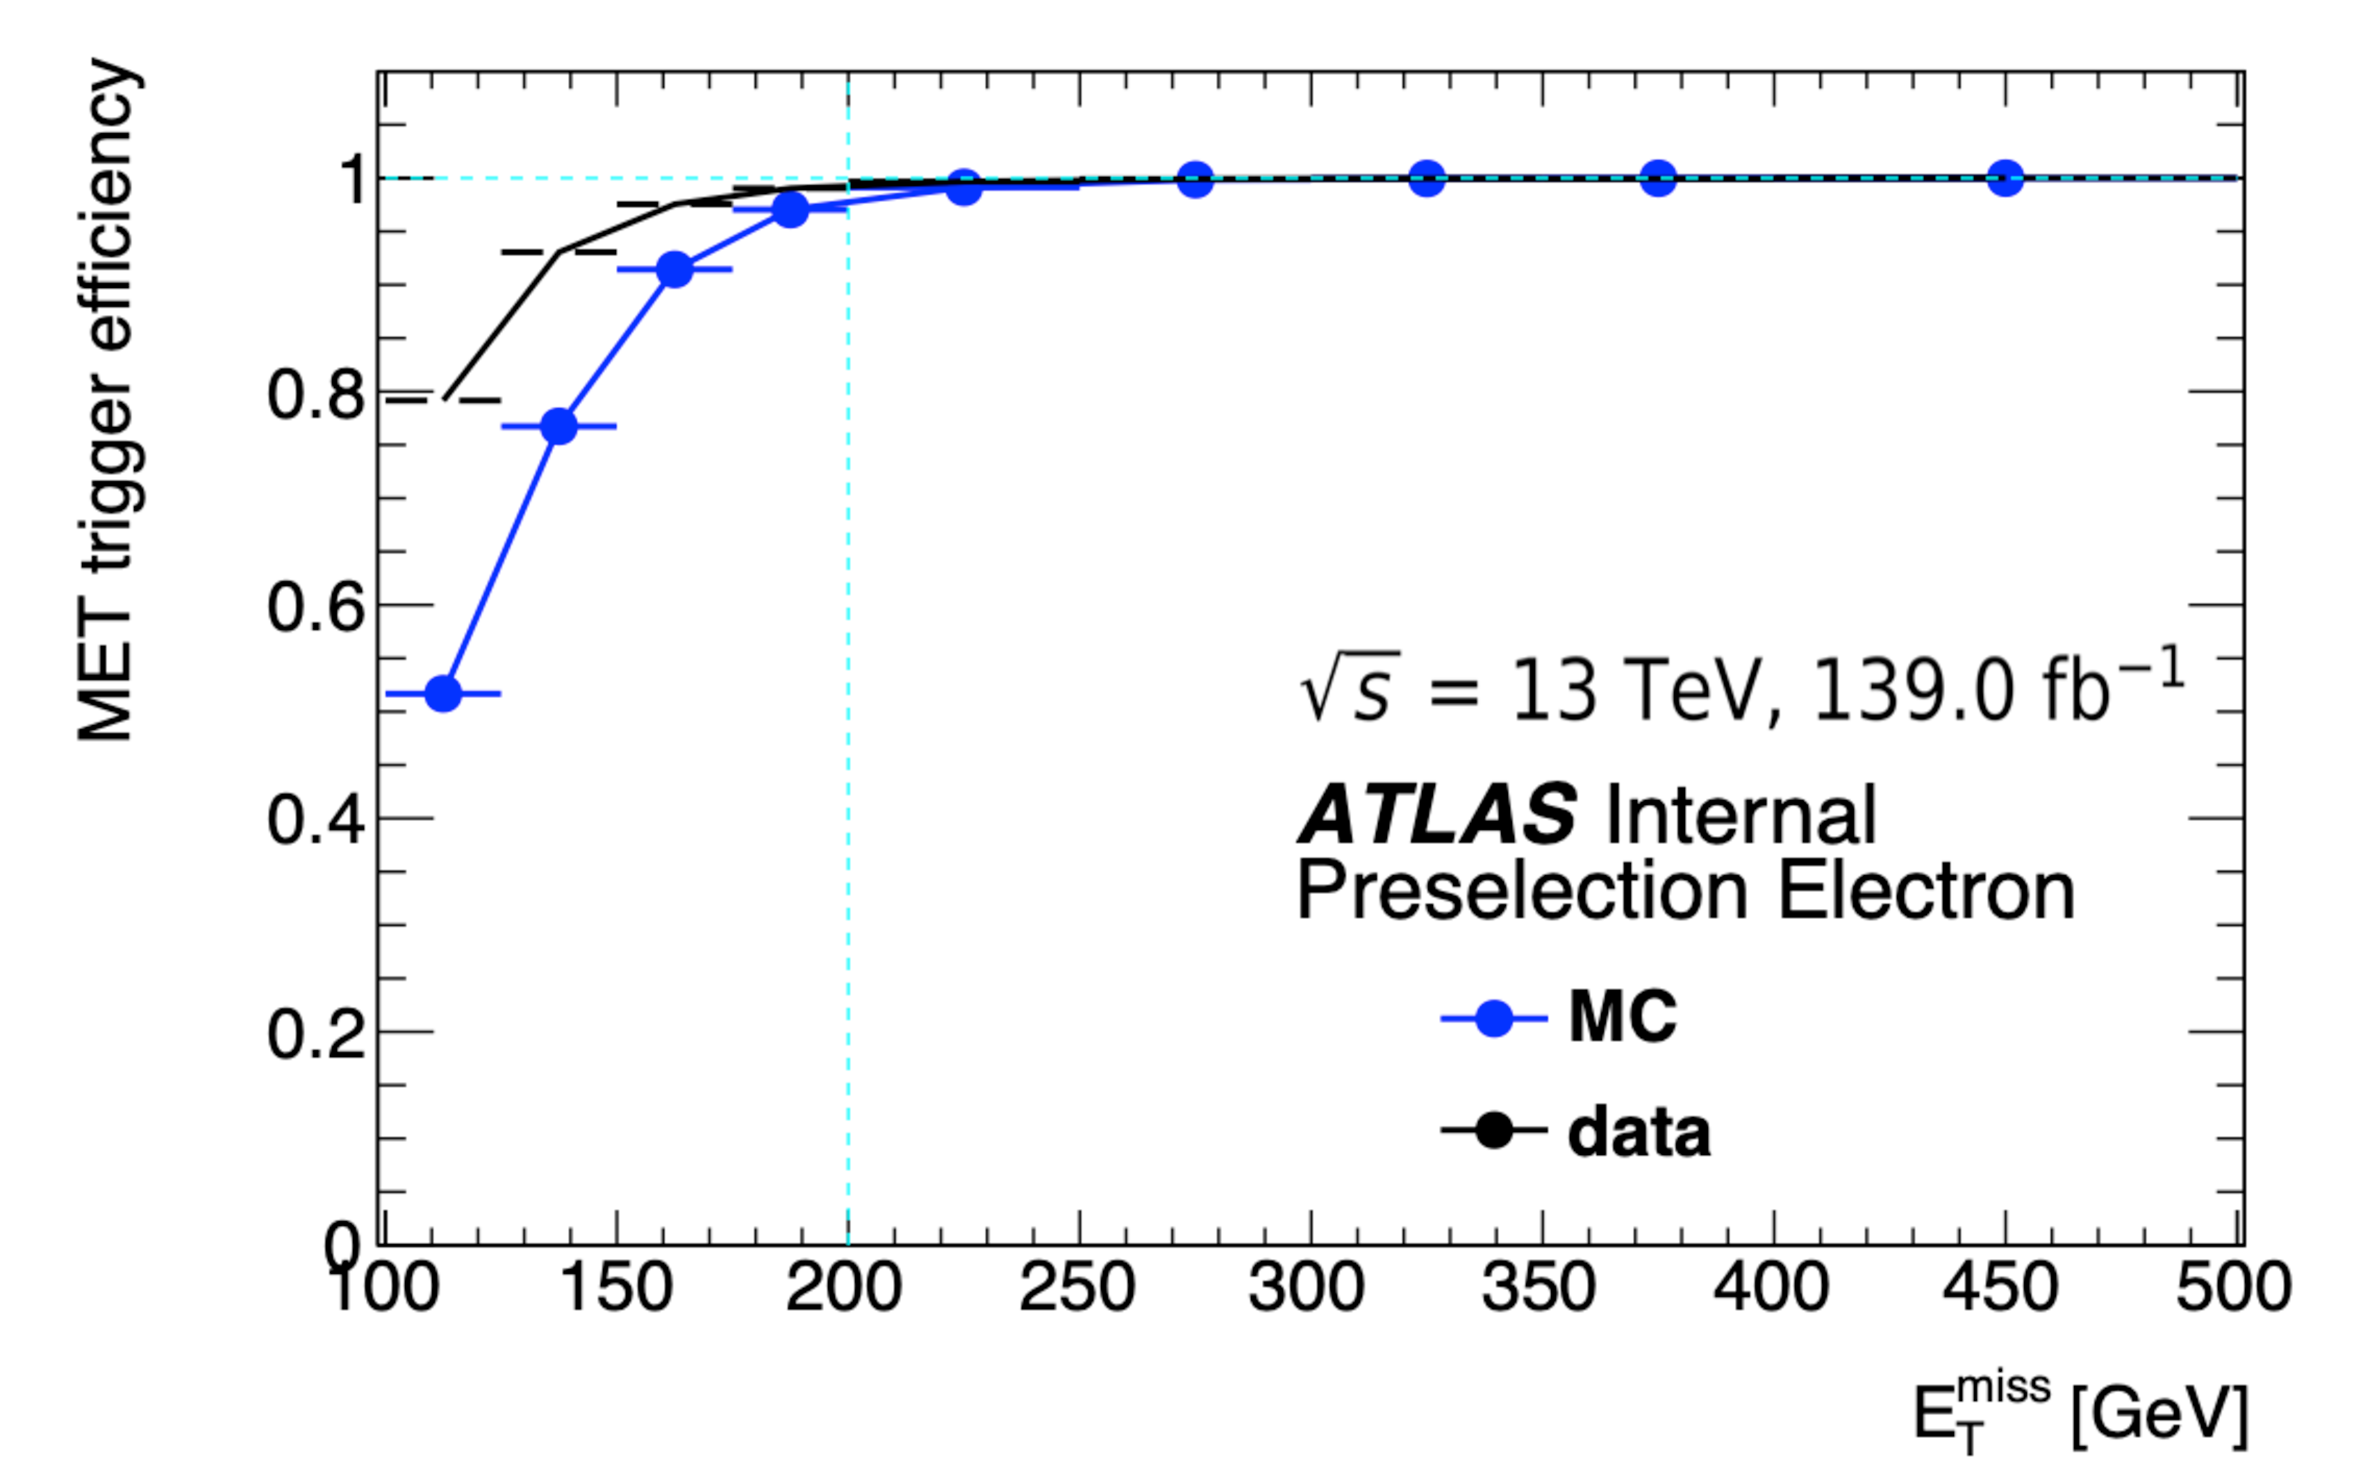
\includegraphics[width = 0.98\textwidth]{Figures/5/METTrigger/PreE_MetTST_met.pdf}
    \caption{Electron Channel}
    \label{ig:mettrig_e}
     \end{subfigure}
    \begin{subfigure}{0.49\textwidth}
     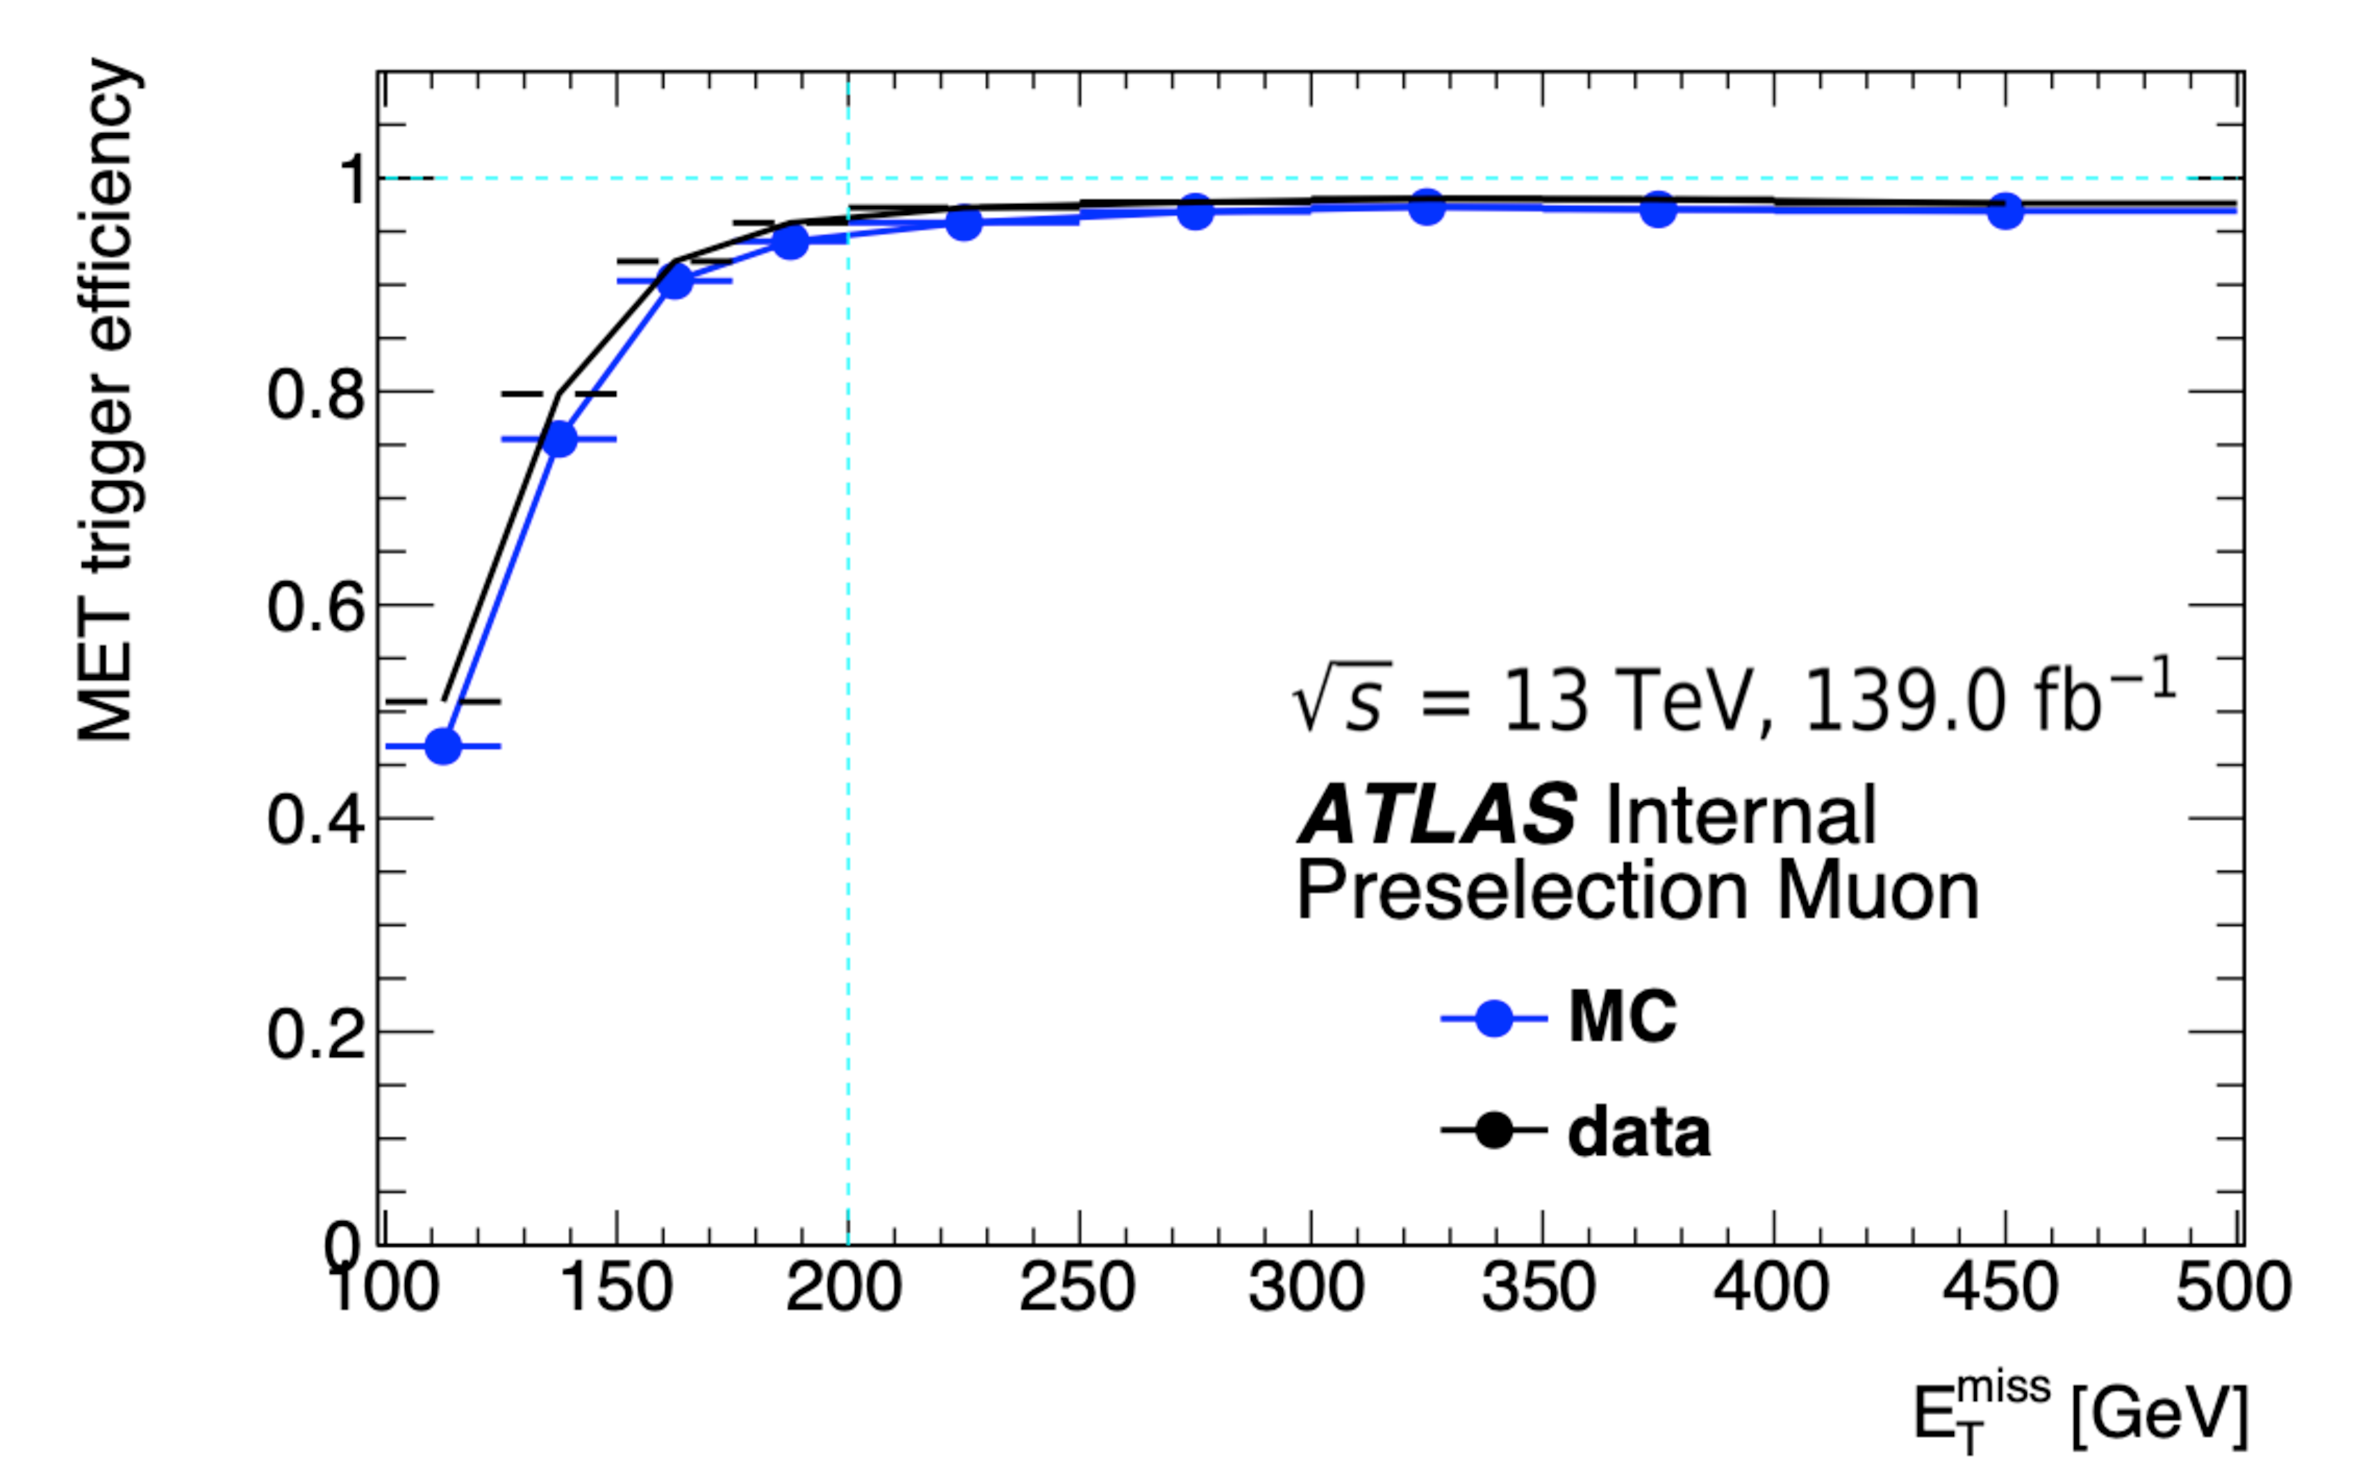
\includegraphics[width = 0.98\textwidth]{Figures/5/METTrigger/PreM_MetTST_met.pdf}
     \caption{Muon Channel}
     \label{ig:mettrig_mu}
     \end{subfigure}
     \caption{Comparison of the \met trigger efficiency defined in Eq. \ref{eq:met_trig_eff}, as a function of the \met lower bound in the event selection, between MC simulated events and ATLAS data in a region defined by a loosened baseline selection. The event selection is separated into electron (left) and muon (right) channels.}
     \label{fig:mettrig}
  \end{figure}
  
Comparing the trigger efficiencies in Figures \ref{fig:mettrig_e} and \ref{fig:mettrig_mu}, the efficiency in the electron channel converges to 100\% for \(\met > 200~\GeV\), but in the muon channel it instead converges to \(\sim90\%\) for \(\met > 200~\GeV\). After some investigation, the inefficiency in the muon channel was found to be due to events which have large \met arising from high-\pt muons. This is because high-\pt muons largely pass through the ATLAS calorimeter and are detected instead by the muon spectrometer. As a result, such high-\pt muon events can be missed by the \met triggers, which don't make use of information from the muon spectrometer \cite{met_performance_2019}. This can be seen by plotting the \met trigger efficiency using a calculation of \met in the event selection that ignores the muon \pt (a.k.a. ``muon invisible") in Figure \ref{fig:metmuinvis}, and observing that in this case the efficiency converges to 100\% for \met (muon invisible) \(> 200~\GeV\). 

\begin{figure}[htbp]
    \centering
     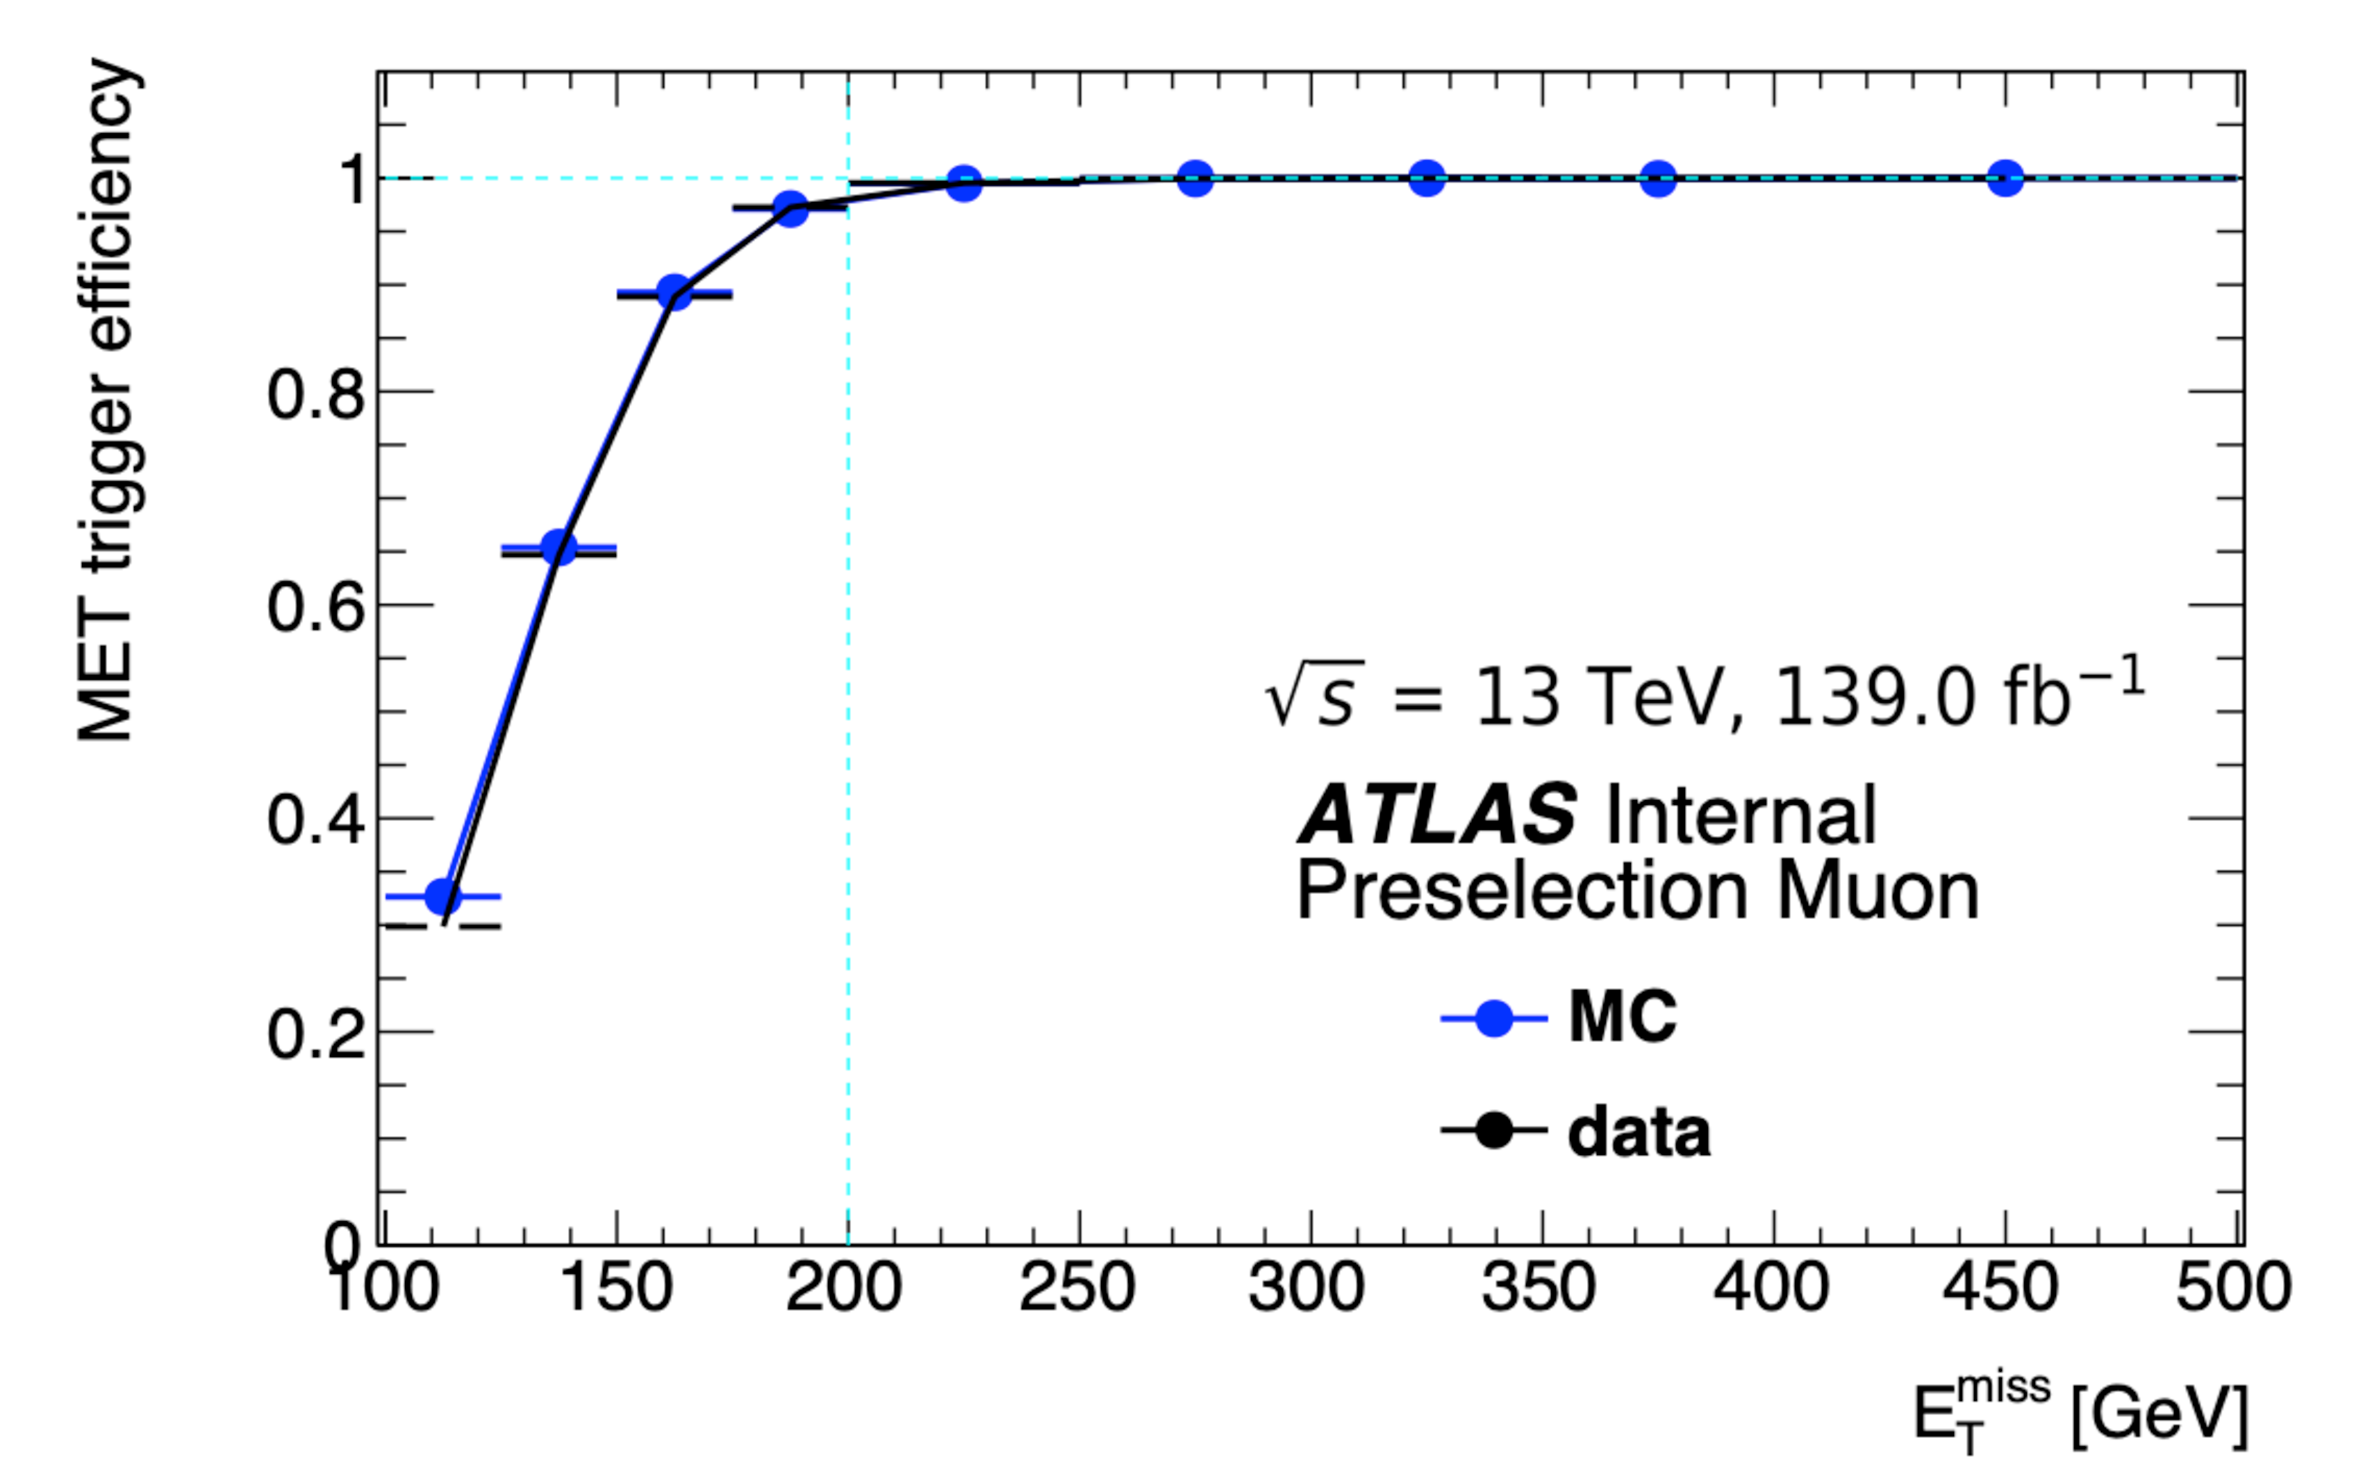
\includegraphics[width = 0.6\textwidth]{Figures/5/TriggerMuInvis/Pre_MetTST_met.pdf}
     \caption{\met trigger efficiency, as a function of the \met lower bound for the loosened baseline event selection in the muon channel, with muons treated as invisible in the calculation of \met}
     \label{fig:metmuinvis}
  \end{figure}
 
As discussed above, events which pass the baseline selection in the muon channel with \(\met > 200 ~\GeV\) but fail the \met trigger generally have large muon \pt. It was found that these high-\met events in the muon channel which fail the \met trigger do, however, pass the muon trigger with high efficiency. For this reason, the efficiency of a logical OR of the \met and single muon triggers is studied in the muon channel. This \met or single muon trigger efficiency is calculated as follows for MC simulated events for a given set of event selection criteria which define a region ``X":

\begin{equation}
\label{eq:met_or_single_muon_trig}
\begin{footnotesize}
\text{eff}_\text{\met OR single muon, MC, region X} = \frac{\sum_i w_i\text{ passing ($\met$ OR single muon triggers)\text{ AND }(in region X)}}{\sum_i w_i\text{ in region X}}
\end{footnotesize}
\end{equation}

\noindent where the event weight \(w_i\) in the numerator includes the scale factors to correct for the known \(<100\%\) trigger efficiency of the single muon trigger. Note that since Eq. \ref{eq:met_or_single_muon_trig} is evaluated only for MC simulated events, there is no need for an independent trigger in the numerator and denominator such as the single lepton trigger included in Eq. \ref{eq:met_trig_eff}. As shown in Figure \ref{fig:trigger_OR}, the \met OR single muon trigger is found to be effectively 100\% efficient, given the application of appropriate scale factors for the single muon trigger, in the muon channel with the loosened baseline event selection for all lower bounds on the \met down to  \(\sim 100~\GeV\).

  \begin{figure}[htbp]
  \centering
    \begin{subfigure}{0.49\textwidth}
     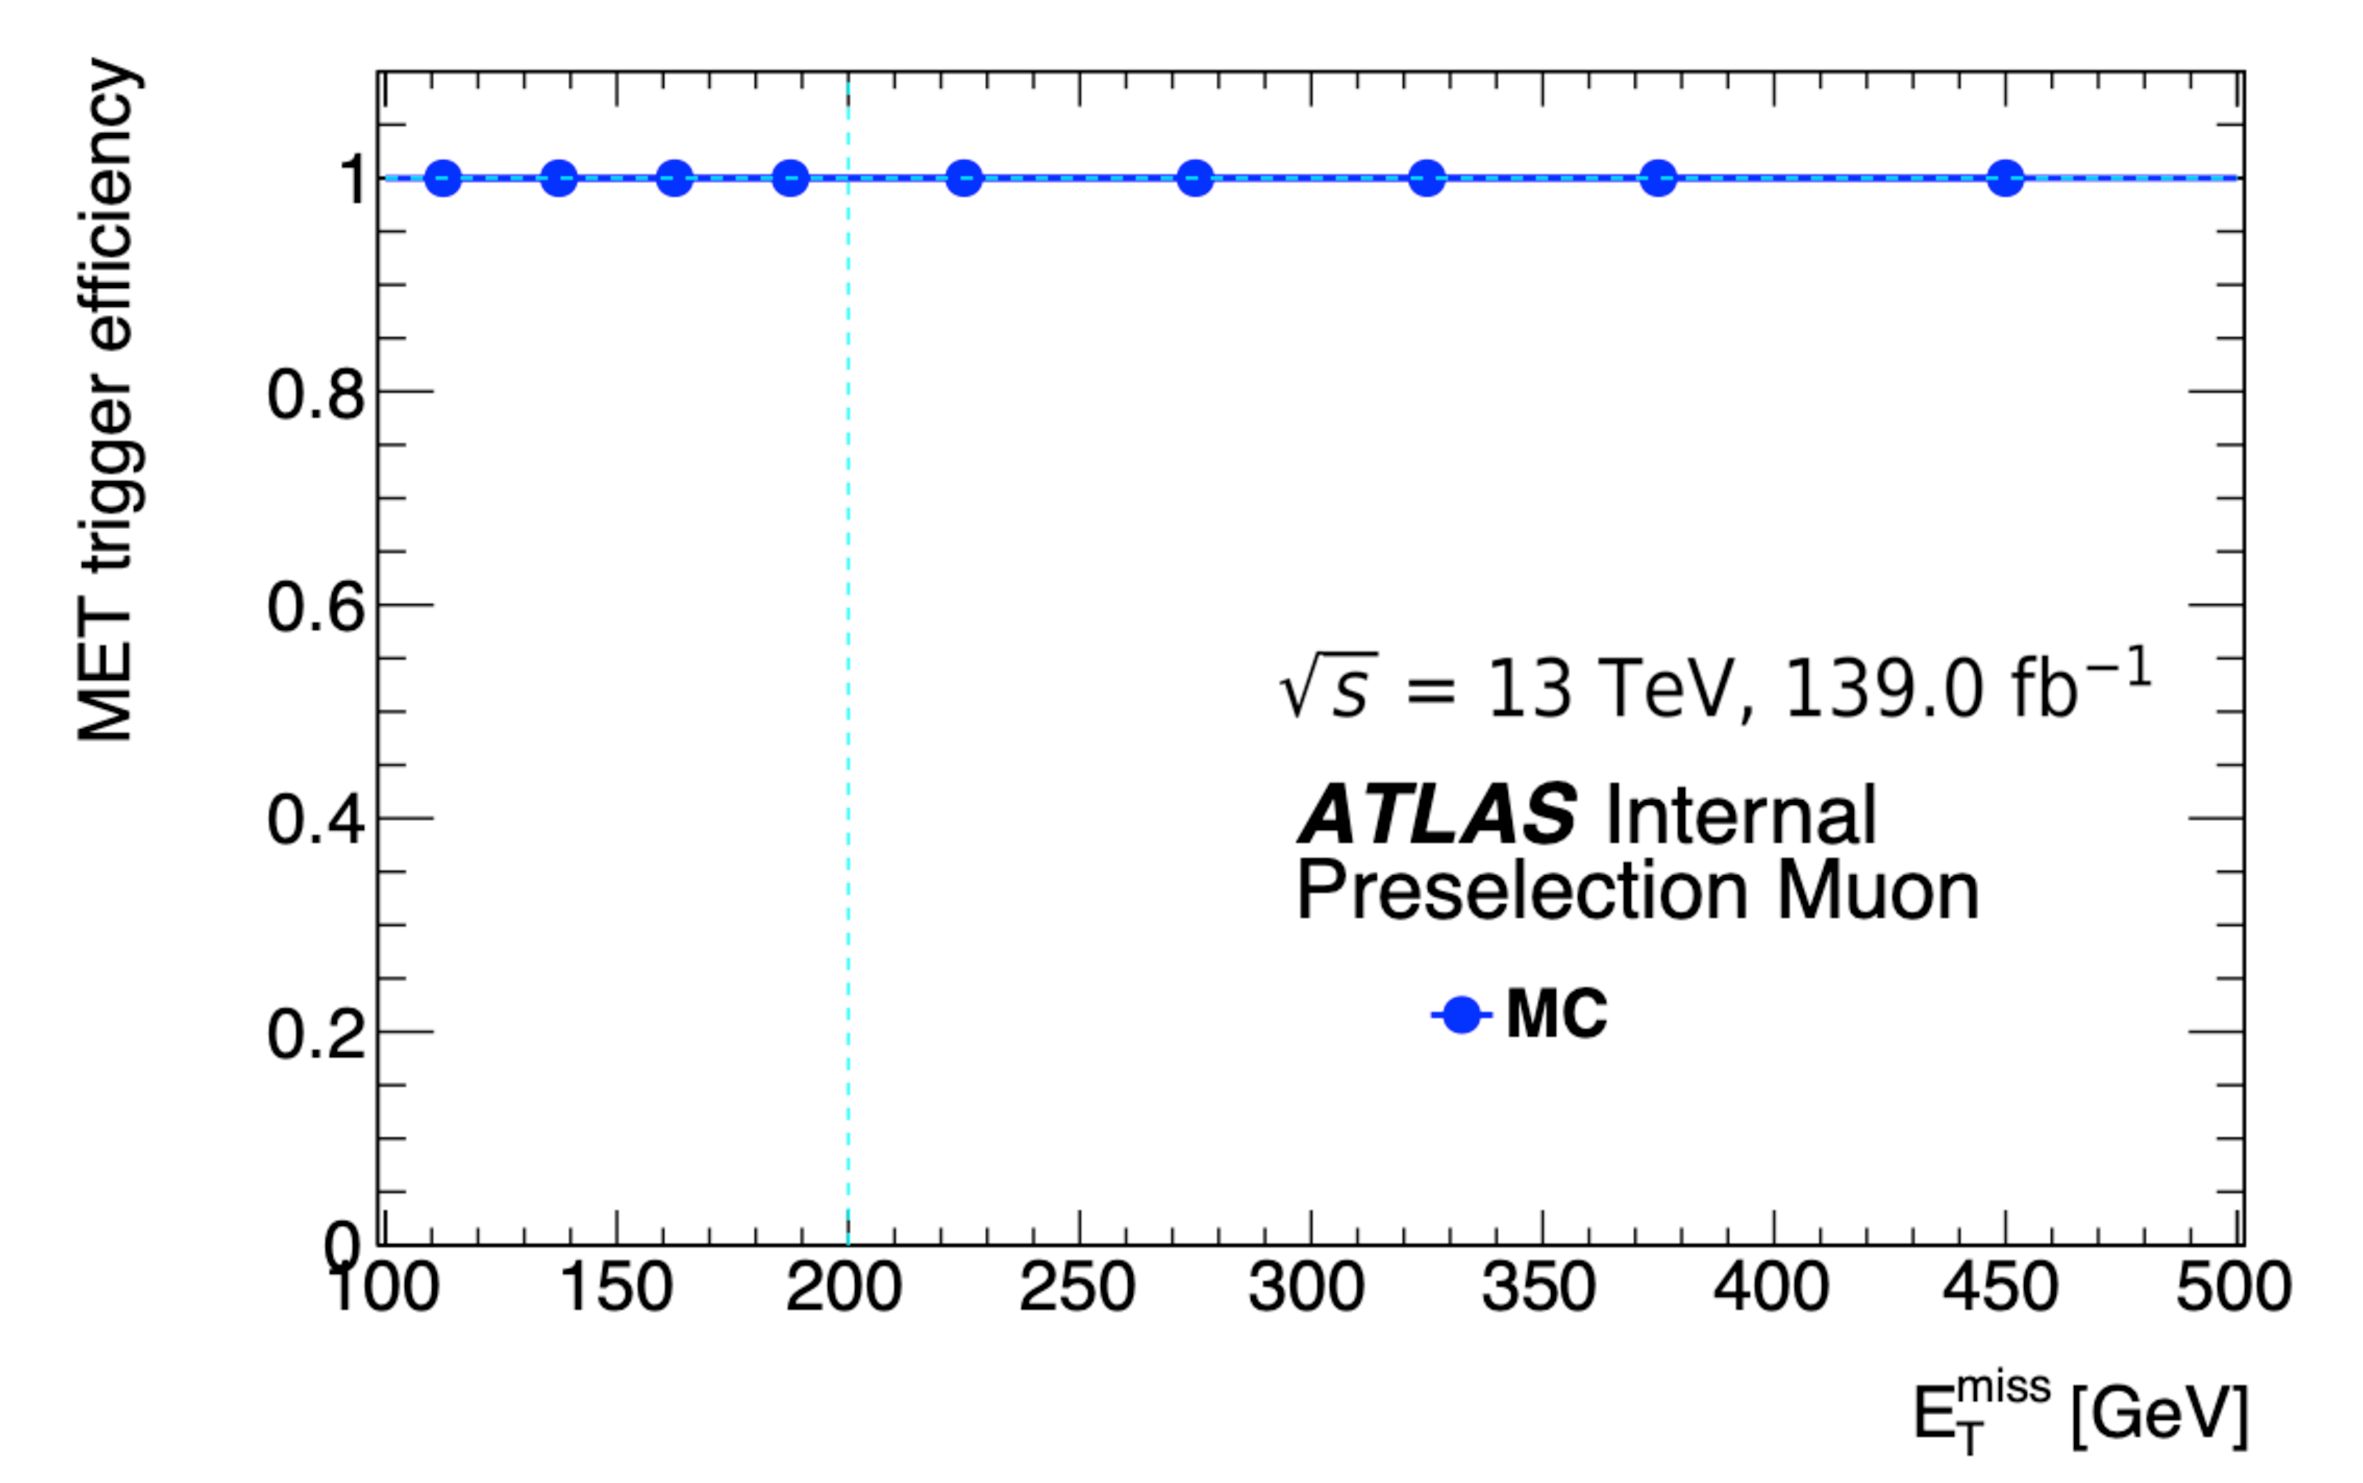
\includegraphics[width = 0.98\textwidth]{Figures/5/TriggerOR/Pre_MetTST_met.pdf}
     \caption{Preselection}
     \end{subfigure}
     \caption{Efficiency of the \met OR single muon trigger, as a function of the \met lower bound, in the muon channel for the loosened baseline event selection in the muon channel.}
     \label{fig:trigger_OR}
  \end{figure}

Based on the analysis presented in this section, it is concluded that, if all events considered in the analysis are explicitly required to have passed the \met or the single muon trigger, the trigger efficiency is known to be 100\% for all events except for the small subset of events with a high-\pt muon which pass the muon trigger but fail the \met trigger. For these events, scaling factors and associated uncertainties, which are determined by independent calibrations performed by the ATLAS collaboration, are included in the event weight to correct for the known \(<100\%\) efficiency of the single muon trigger. An additional ``trigger-matching" requirement is applied for events which fail the \met trigger but pass the single muon trigger. This trigger matching requires that the final state muon object that was reconstructed during data-taking and which activated the single muon trigger can be identified as the same muon object (i.e. as having originated from the same muon) that was later reconstructed with the more granular offline reconstruction software. 
